\chapter{Searching for Supersymmetry with $\alpha_{T}$ in all-hadronic events}
The analysis presented here represents a model-independent search for new physics in the all-hadronic channel, where the final state is defined by the presence of jets and missing energy. Designed to search for signs of supersymmetry whilst remaining sensitive to other new physics models, an inclusive strategy is used imposing restrictions only on the final state.  Events are chosen based on their compatibility with a topology of heavy new particles pair-produced in p-p collisions, which decay through a chain with an end product which is stable and undetectable. 

Isolating these new physics events from Standard Model background processes is essential in order to identify an excess. Controlling the dominant background from QCD Multijet processed is the central feature of the strategy, implementing use of the powerful discriminant, the \alt variable described in Chapter \ref{ch:at}. The remaining backgrounds from electroweak processes may then be accounted for using data-driven estimation techniques in muon and photon control samples. 



\section{Samples}
This analysis uses datasets both from Monte Carlo simulation (MC) and of data recorded by the CMS detector in 2011.

\subsection{Monte Carlo Simulation}
Datasets of simulated events with calculated cross-sections are required for any analysis at the LHC. Due to the hadron-collider nature these rely on the PDF's 
\subsubsection{Standard Model Background}
\begin{description}
\item[QCD Multijet]{}
\item[W + jets]{}
\item[Z $\ra \nu\bar{\nu}$ + jets]{}
\item[t$\bar{\textrm{t}}$]{}
\end{description}
\subsubsection{CMSSM SUSY Signal}
For the purpose of understanding the possible yields from CMSSM SUSY, two mSUGRA parameter points are used. CMS has a dedicated set of 10 Low Mass(LM) points designed for initial data-taking from which we have chosen LM4 and LM6, the values of which are found in Table~\ref{tab:LM}. 

\begin{table}[htbp]
\centering
\begin{tabular}{c c c c c c }
\hline
\hline
\textbf{mSUGRA Point} & $m_{0}$ & $m_{1/2}$ & $A_{0}$ & tan $\beta$ & sign$(\mu) $  \\
\hline
\hline
\textbf{LM4} & 210 GeV & 285 GeV  & 0 & 10 & + \\
\textbf{LM6} & 85 GeV & 400 GeV & 0 & 10 & +\\
\hline
\end{tabular}
\caption{\label{tab:LM}The two CMSSM SUSY signal points used and their corresponding mSUGRA parameter values.}
\end{table}

These points are chosen for their existence above the exclusion limit set previously, shown in Figure~\ref{fig:lm35limit} on the exclusion plot from the 2010 iteration of this analysis\cite{35paper}.

\begin{figure}[htbp]
\centering
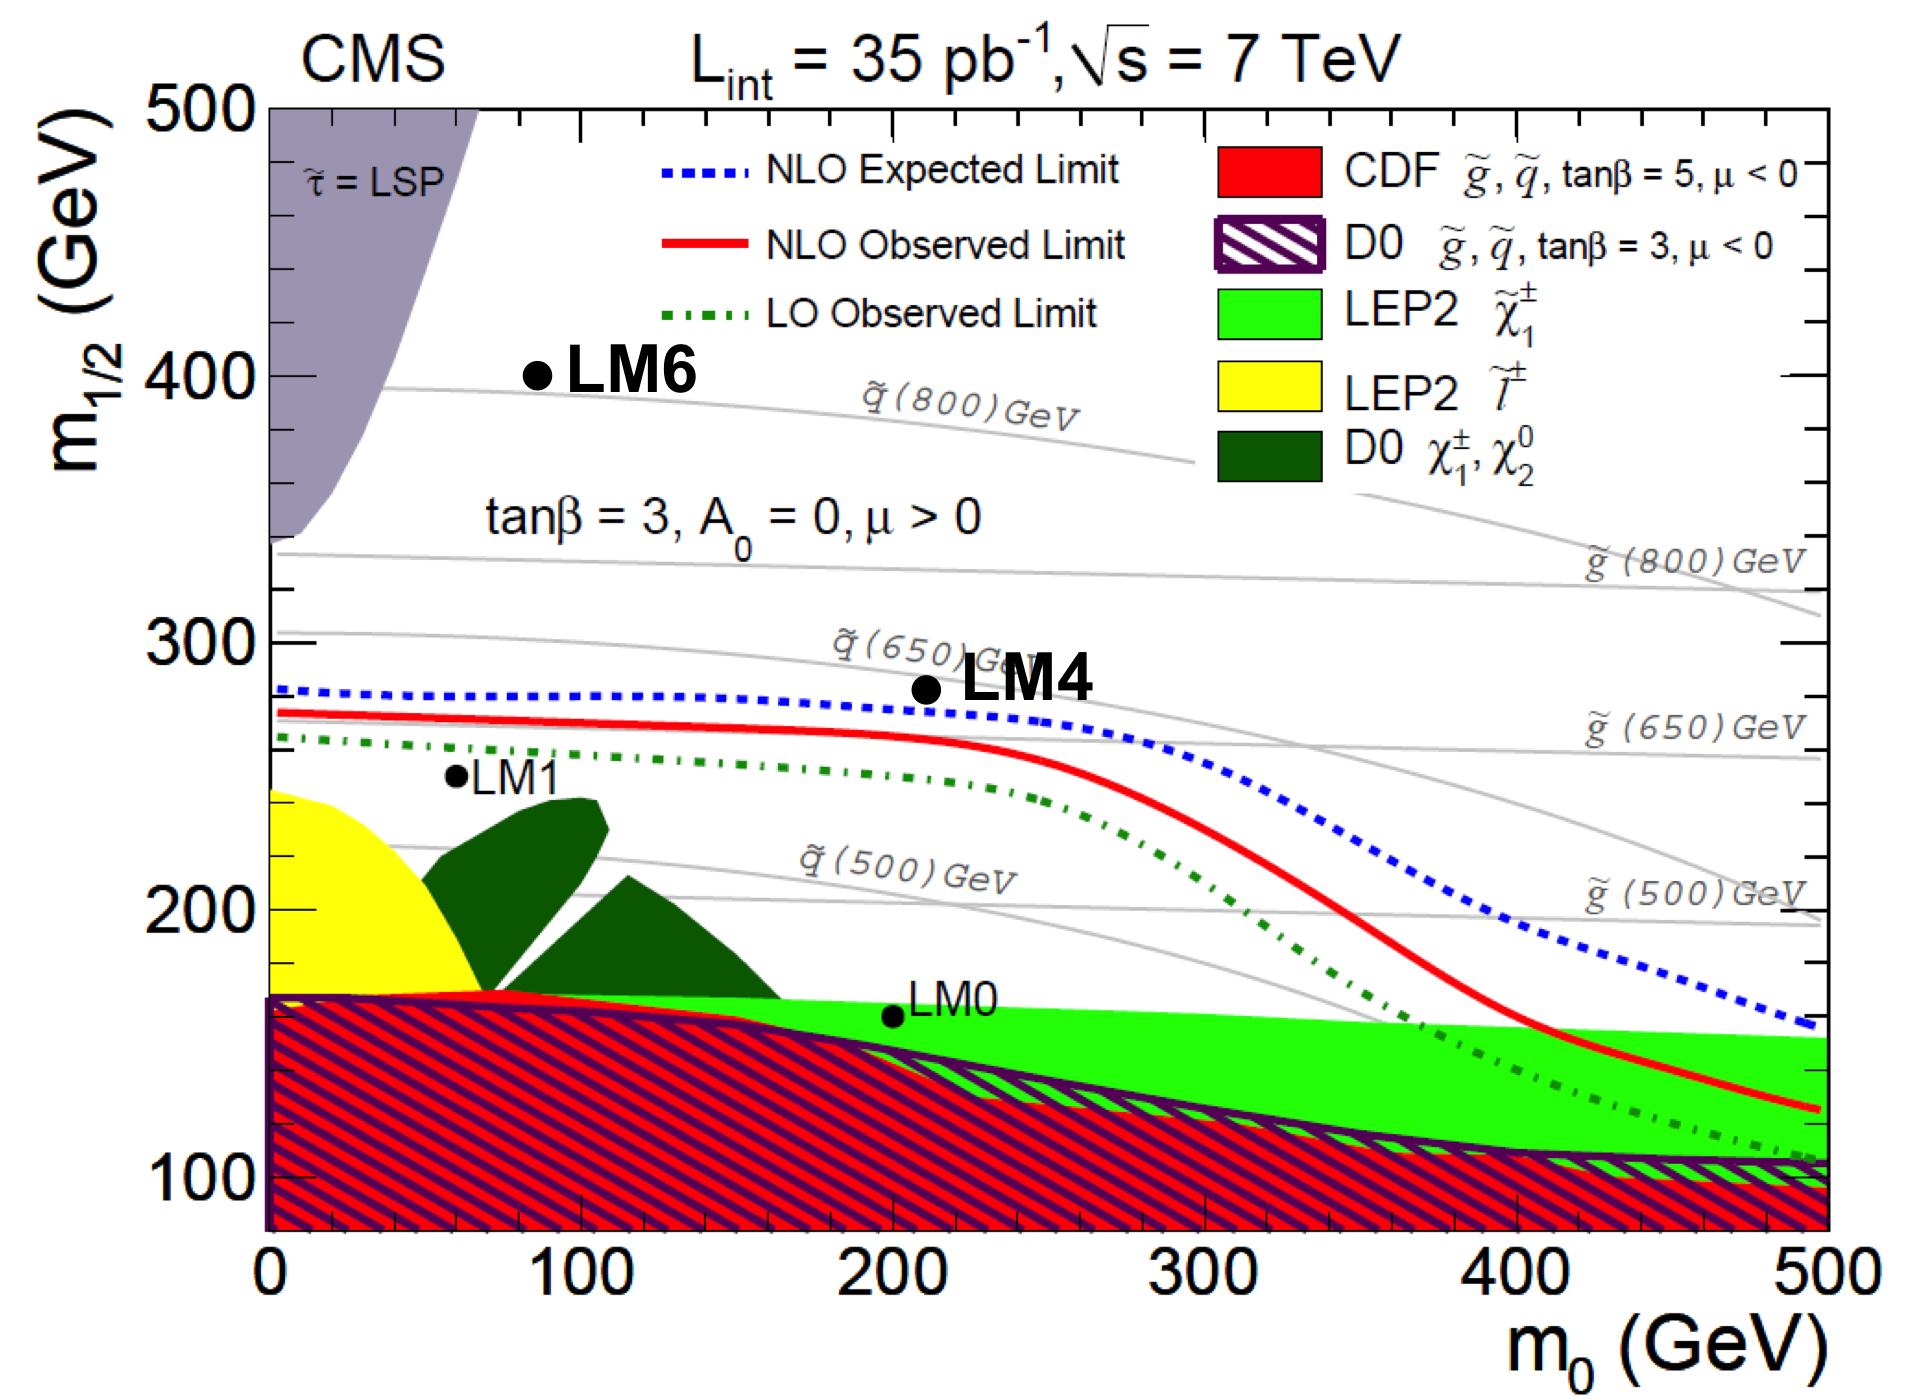
\includegraphics[width=0.70\textwidth]{Figures/Analysis/LM46on35limit}
\caption{\label{fig:lm35limit}The exclusion limit set in the previous incarnation of this analysis with the 35pb$^{-1}$ 2010 CMS dataset shown in the $m_{0}-m_{1/2}$ plane with tan $\beta$ = 10, $A_{0}$ = 0 and sign$(\mu)$ = +. Reference points LM4 and LM6 to be used in the 2011 analysis are illustrated, in the region yet to be excluded. Previously used reference points LM0 and LM1 are shown below the limit already excluded~\cite{35paper}.}
\end{figure}

\subsection{Data Sample}
\label{sec:datasam}
This analysis considers data collected by CMS at $\sqrt{s} = 7$~TeV in 2011 between March and June, during the data-taking period known locally as Run2011A. Analyses use only the data taken whilst CMS was fully operational, and thus the data used were specified by the certified list of ``good runs" that correspond to 1.1$fb^{-1}$ of integrated luminosity. 

As described previously, loose requirements on the types of triggers passed allow the sorting of the data into each Primary Dataset (PD). For the hadronic analysis the HT dataset is used, with basic low-threshold $\HT$ triggers required. Higher threshold triggers are applied subsequently as part of the analysis selection, detailed in Section~\ref{sec:trig}. 

For the data-driven estimation techniques muon and photon control samples are defined. For the muon control sample, the HT PD is also used, as a low muon $p_{T}$ requirement makes this better suited than the dedicated Muon PD. However the photon control sample uses the dedicated Photon PD that requires some basic threshold photon triggers to be passed. 


\section{Analysis Framework}

For the purpose of the analysis private ntuples are generated fro the RECO samples using the CMSSW framework and CMS's Physics Analysis Toolkit (PAT), retaining all variables from the intermediate step of PAT-tuples recommended by the CMS SUSY group. Followng this private code is used on the ntuples to perform the analysis.   



\section{Trigger}
\label{sec:trig}
In order to select the signal events and minimise the contamination from backgrounds, a set of selection criteria is applied. As described previously in Section~\ref{sec:detrig}, data collected by the CMS detector is stored and organised according to the L1 and HLT trigger paths passed. While the datasets chosen in Section~\ref{datasam} have some basic level trigger requirements, we also require a more stringent set of requirements. 


In the previous iteration of this analysis for the 2010 dataset, a set of pure \HT triggers was used. However these are unsuitable for the 2011 analysis as due to the increase in instantaneous luminosity the rate of triggers with desirable thresholds have become too high and become prescaled, rendering them unsuitable for the signal selection, although they will play a part in the control region. Moving to higher \HT thresholds is also undesirable as it would reduce a significant portion of the search region. 

The use of cross-object triggers is now employed, requiring events that pass thresholds in both \HT and \mht for the signal region. As the era of data-taking progressed there were several menu-changes, during which time we required the lowest un-prescaled thresholds available at a given time to ensure signal yields are accurate, some of which are implemented in the menu under different versions, the relevant paths appended with \verb!_v*!. 

The first set of runs in the 2011 dataset correspond to a trigger used with thresholds in [\HT,\MHT] = [260,60]~GeV.  After this the CMS standard thresholds were shifted down by 10~GeV, relevant for the major portion of data taking. For all runs henceforth the lowest unprescaled cross-trigger had an \HT threshold of 250 GeV, during which time the \MHT thresholds of the lowest unprescaled evolve through 60, 70 and 90 GeV. 

\begin{table}[htbp]
\centering
\begin{tabular}{c}
\hline
\hline
HLT Trigger Path\\ 
\hline
\hline
\verb!HLT_HT260_MHT60_v2!\\
\verb!HLT_HT250_MHT60_v2!\\
\verb!HLT_HT250_MHT60_v3!\\
\verb!HLT_HT250_MHT60_v4!\\
\verb!HLT_HT250_MHT70_v1!\\
\verb!HLT_HT250_MHT70_v3!\\
\verb!HLT_HT250_MHT70_v4!\\
\verb!HLT_HT250_MHT90_v1!\\
\hline
\end{tabular}
\caption{\label{tab:sigtrig}List of HLT trigger paths for the signal selection from which the lowest unprescaled was used or any given run.}
\end{table}

The quantities \HT and \MHT used in the trigger requirements differ from those used in the analysis. The trigger uses jets built in online reconstruction with uncorrected energy to form these quantities, whereas those quantities in our analysis use only jets passing the object requirements and with corrected energy. Thus it is not the case that an \HT trigger of threshold X is efficient for events with \HT > X in the analysis. It is necessary to ensure the trigger is efficient with regard to analysis cuts in both \HT and \MHT. 

In this two step process, the efficiencies of pure \HT triggers of thresholds 250 and 260 are identified through comparison to an orthogonal sample, using a Muon \HT cross trigger. These triggers can be considered 100\% efficient by an offline \HT cut of 275 GeV, and thus this is selected for the analysis. Having made this cut the efficiency of the \MHT part may be tested, with reference to \alt (which is analogous to a cut on MHT). In the lowest bin of the analysis, $275 < \HT < 325$~GeV a small inefficiency was measured of 0.99$^{+0.01}_{0.02}$, and in all other bins $\HT > 325$ the analysis is measured as fully efficient - 1.0$^{+0.00}_{-0.03}$.  

This analysis makes use of those events which fail the \alt selection criteria also, as the hadronic bulk control sample. In this region the chosen signal triggers would not be efficient as we wish to use the events with low \MHT which would not pass that element of the trigger requirement. Here the pre-scaled \HT triggers are suitable for use, taking into account the prescale factors to gain yields in this bulk sample, an approach which is suitable due to the high statistics from QCD events. The lowest prescale of the trigger thresholds chosen for each \HT bin, shown in Table~\ref{tab:bulktrig}, are used at each point in the evolution of the trigger menu.  


\begin{table}[htbp]
\centering
\begin{tabular}{ c c }
\hline
\hline
Analysis $H_{T}$ Region & HLT Trigger Paths\\
\hline
\hline
$275 < \HT < 325$ & \verb!HLT_HT250_v*, HLT_HT260_v* !\\
$325 < \HT < 375$ & \verb!HLT_HT300_v*!\\
$375 < \HT < 475$ & \verb!HLT_HT300_v*, HLT_HT350_v* !\\
$475 < \HT < 575$ &\verb!HLT_HT440_v*, HLT_HT450_v* !\\
$\HT > 575$ & \verb! HLT_HT520_v*, HLT_HT550_v*!\\
\hline
\end{tabular}
\caption{\label{tab:bulk trig}The prescaled HLT trigger paths used for each $\HT$ region of the hadronic control sample, where \alt < 0.55.  N.B. The $\HT$ that defines the region is built from jets with corrected energy that pass the requirements of the analysis, while the \HT quoted in the trigger definition is uncorrected and built using online reconstruction jets available to the trigger.}
\end{table}



In the muon control sample, due to the low $p^{\mu}_{T}$ = 10~GeV threshold we use the same triggers as for the hadronic signal sample. The photon sample makes use of the single photon trigger paths shown in Table~\ref{tab:photrig}, using the lowest unprescaled threshold available for each given run in the data.
\begin{table}[htbp]
\centering
\begin{tabular}{ c }
\hline
\hline
HLT Trigger Paths\\
\hline
\hline
\verb!HLT_Photon75_CaloIdVL!\\
\verb!HLT_Photon75_CaloIdVL_IsoL!\\ 
\verb!HLT_Photon90_CaloIdVL!\\
\verb!HLT_Photon90_CaloIdVL_IsoL!\\
\hline
\end{tabular}
\caption{\label{tab:photrig}The list of HLT trigger paths available used to select the events for the Photon Control sample from which the lowest unprescaled photon threshold is selected in any given run.}
\end{table}


Events passing the relevant triggers proceed into the analysis selection.

\section{Object Definitions}
\subsection{Good Event Definition}
\label{sec:good}
In order for an event to be considered suitable for use in physics analyses, it must be defined as a ``Good Event". Such an event is required to have at least one non-fake good primary vertex with $N_{dof}$ $>$ 4. Constraints on the vertex position along the beam axis $|z_{vtx}| <$ 24 cm and perpendicular to the axis of $\rho <$ 2 cm must be satisfied. Events that have many fake tracks are identified as monster events and removed, by requiring that the ratio of High Purity tracks to the total number be greater than 25\% in events with more than 9 tracks. 


\subsection{Jets}
\label{sec:jetsel}
The jets used in this analysis are Calo Jets, reconstructed as described in Section~\ref{sec:reconjet} using the anti-k$_{T}$ jet clustering algorithm. In addition, a reconstructed jet must pass an additional selection in order to be considered for the analysis:
\begin{itemize}
\item Corrected jet transverse momentum requirement of \Pt $>$ 50~GeV 
\item Jet pseudo-rapidity $|\eta| < 3$ required to ensure within the fiducial range of the calorimeter systems. 
\item Passes``loose" jet identification criteria to reject jets resulting from unphysical energy using cuts in Table \ref{tab:jetid}. 
\end{itemize}

\begin{table}[htbp]
\centering
\begin{tabular}{ m{6.6cm}  c  c }
\hline
\hline
 \centering Definition & Variable & Cut \\
\hline
\hline
 \centering Fraction of jet energy contributed by the ``hottest" hybrid photo-diode &  $f_{HPD}$ & $< 0.98$ \\
 %\hline
 \centering Minimum number of cells required to contribute 90\% of the jet energy & $N^{90}_{cells}$ & $\leq$ 2 \\
 %\hline
 \centering Fraction of jet energy contributed by deposits in ECAL & $f_{EM}$ & $> 0.01$ \\
 %\hline
\multirow{2}{6.9cm}{Balance of the energy measured in the short($E_{S}$) and long$(E_{L})$ HF fibers.} &  $R_{HF} = \frac{(E_{S} - E_{L})}{ (E_{S} + E_{L})}$ & $R_{HF} > - 0.9$\\
& (if  $p_{T}^{jet}>$ 80~GeV)  &             ($-0.9 < R_{HF} < 1$)\\
\hline
\end{tabular}
\caption{\label{tab:jetid} Set of cuts applied in ``loose" CaloJet ID used to reject jets resulting from fake calorimeter deposits representing unphysical energy. Devised using cosmic run data as a pure sample of non-collider ``fake" jets, full details of which can be found in \cite{JME-09-008}}
\end{table}


Any jet which passes the $\Et$ and $\eta$ requirements but fails the ``loose" identification criteria is noted, and the event is marked as containing an ``odd" jet, as the presence of such a particle reflects an event whose kinematics are poorly understood and may therefore lead to a misleading \MHT.
\subsection{$\HT$ and \MHT}
The calculation of both \HT and \MHT is performed using only the jets selected by the selection above in Section~\ref{sec:jetsel}.

\subsection{Muons} 
Although muons are not required by the analysis, a veto on them must be employed, based on muons that satisfy the following set of criteria:
\begin{itemize}
\item $p^{\mu}_{T} >$ 10~GeV
\item $| \eta|$ $<$ 2.5
\item Relative Combined Isolation = $(Iso_{tracker} + Iso_{ECAL} + Iso_{HCAL}) / p^{\mu}_{T} < $0.15\footnotemark
\item Passes ``tight" muon identification, using cuts shown in Table~\ref{tab:muid}.
\end{itemize}
\footnotetext{The components $Iso_{tracker}$($Iso_{ECAL}, Iso_{HCAL})$ represent the sum of \Pt($E_{T}$) in the relevant detector component, calculated in a cone of R = 0.3 in $\eta-\phi$ around there muon trajectory. The track hits used to reconstruct the muon are not used and any muon deposit in the calorimeters is removed via a smaller veto cone.}

\begin{table}[htbp]
\centering
\begin{tabular}{ m{8.9cm}  c  c }
\hline
\hline
 \centering Definition & Variable & Cut \\
\hline
\hline
 Reconstructed with outside-in algorithm & Global Muon & Required\\
  %\hline
Reconstructed with inside-out algortithm & Tracker Muon & Required\\
% \hline
 Global muon track fit quality & $\chi^{2}$ & $< 10$ \\ 
 %\hline
Number of hits in the silicon tracker included in track & $N^{hits}_{\textit{trk}}$ &$ >$ 10\\
%\hline
Number of pixel hits in $N^{hits}_{trk}$ & $N^{hits}_{\textit{pixel}}$ & $ > $ 0\\
Number of hits in muon system included in Global Muon & $N^{hits}_{\textit{muon}}$ & $\geq $ 1\\
Transverse impact parameter with respect to vertex & $d_{xy}$ & $< $ 2~mm\\
\hline
\end{tabular}
\caption{\label{tab:muid} Set of cuts applied in ``tight" Muon ID, taken from \cite{MUO-10-002}}
\end{table}



\subsection{Electrons}
Similarly electrons are also defined for veto purposes, with the definition of an electron in the analysis as that passing the following cuts:

\begin{itemize}
\item $E^{e}_{T} > 10 GeV$
\item $|\eta| < 2.5$
\item Combined Isolation = $(\sum_{tracker} p_{T} + \sum_{ECAL}E_{T} + \sum_{HCAL}E_{T})/p^{e}_{T} < 0.15$
\item Pass WP95 electron identification implemented using cuts in Table~\ref{tab:eid}.
\end{itemize}

\begin{table}[htbp]
\centering
\begin{tabular}{ m{6.9cm}  c  c  c}
\hline
\hline
 \centering Definition & Variable & Barrel Cut & End-Cap Cut \\
\hline
\hline
RMS of the width in $\eta$ of the crystals about the most energetic crystal in the seed& $\sigma_{i \eta i \eta}$ & $<$ 0.01 & $<$ 0.03\\
Difference in $\phi$ between track and supercluster&$\Delta \phi_{vtx}$& $<$ 0.8 & $<$ 0.7 \\
Difference in $\eta$ between track and supercluster& $\Delta \eta_{vtx}$& $<$ 0.007 & $<$ 0.01\\
Ratio of HCAL energy in $\Delta R = 0.15$ to ECAL seed energy & H / E & $<$ 0.15 & $<$ 0.07\\
\hline
\end{tabular}
\caption{\label{tab:eid} Set of cuts applied in ``WP95" Electron ID, taken from \cite{AN-10-116} corresponding to an intended 95\% efficiency for signal electrons in W events for electrons with $p_{T} > 20$~GeV.}
\end{table}
\footnotetext{where electron $p_{T} > 20$~GeV, measured with a sample of $W \ra e$ events.}
\subsection{Photons}

Photons in the analysis are defined by the following set of requirements:
\begin{itemize}
\item $p_{T}^{\gamma} > $ 25~GeV
\item $|\eta| < 2.5$
\item Passes ``tight" photon cut-based identification (including isolation) using cuts shown in Table~\ref{tab:pid}.
\end{itemize}


\begin{table}[htbp]
\centering
\begin{tabular}{ m{6.9cm}  c  c  c}
\hline
\hline
 \centering Definition & Variable & Barrel Cut & End-Cap Cut \\
\hline
\hline
Tracker Isolation in a cone of R=0.4 & $Iso_{trk}$ & \multicolumn{2}{c}{$< (2.0 GeV + 0.001E_{T}^{\gamma})$}\\
ECAL Isolation in an outer cone of R=0.4 (inner cone R=0.06 removed). & $Iso_{ECAL}$ & \multicolumn{2}{c}{$< (4.2 GeV + 0.006E_{T}^{\gamma})$}\\

HCAL Isolation in an outer cone of R=0.4 (inner cone R=0.15 removed). & $Iso_{HCAL}$ & \multicolumn{2}{c}{$< (2.2 GeV + 0.0025E_{T}^{\gamma})$}\\

RMS of the width in $\eta$ of the crystals about the most energetic crystal in the seed& $\sigma_{i \eta i \eta}$ & $<$ 0.013 & $<$ 0.030\\
Ratio of HCAL energy in $\Delta R = 0.15$ to ECAL seed energy & H / E & $<$ 0.05 & $<$ 0.05\\
\hline
\end{tabular}
\caption{\label{tab:pid} Set of cuts applied in ``tight" Photon ID, taken from \cite{EGM-10-006}}
\end{table}

\section{Pre-Selection}
A basic selection of events used for comparison of distributions between data and monte-carlo events shall be known as "pre-selection",  following the details set out in this section.

\begin{description}


\item[HCAL Barrel and End-cap (HBHE) Noise Fiter]{Events where noise has been identified in the HCAL are removed also, using an algorithm which checks for Photodetectors which have at east 17 out of 18 channels with an E $>$ 1.5 GeV.}
\end{description}
Following these conditions events are then selected by the following criteria, using the definitions of physics objects according to the criteria stated previously:

\begin{itemize}
\item Pass triggers as detailed in Section~\ref{sec:trig}.
\item Pass Good Event selection as detailed in Section~\ref{sec:good}.
\item{Require events with N$_{jet}$ $\geq$ 2}
\item N$_{muon}$ = N$_{electron}$ = 0 to reduce the effects of missing energy from neutrinos.
\item N$_{photon}$ = 0 to ensure a pure hadronic set of events.
\item Events with $>$ 0 ``odd" jets are vetoed.
\item Additional constraint on the transverse momentum of the two leading jets $p^{j1}_{T},p^{j2}_{T} >$ 100~GeV.
\item Additional constraint on the leading jet pseudorapidity $|\eta^{j1}| <$ 2.5.
\item \HT $\geq$ 275 GeV 
\end{itemize}



\section{Final Signal Selection}

After the preselection a final set of cuts is applied, including the \alt cut that defines the signal region alongside cleaning cuts which remove events that may lead to inaccurate results. 

\begin{itemize}
\item \alt $>$ 0.55
\item{If the ratio R$_{miss}$ = \mht / \met $>$ 1.25, the event is rejected. This protect the quantity \alt from the scenario where many jets fail the $p_{T}$ = 50~GeV threshold thus resulting in fake \mht and thus misleading values of \alt. }
\item{To prevent against fake missing energy resulting from dead or masked cells in the ECAL or the gap between the barrel and end-caps the following procedure is used: The jet most likely to be responsible for the \MHT is found. If the angle $\phi$ between this jet and the vector $\vec{\MHT}$ (known as $\Delta \phi*$) less than 0.5 then the $\eta-\phi$ distance between the jet and the nearest masked ECAL cell is computed, along with the distance from the detector gap. If either distance is smaller than 0.3 then the event is rejected. }

\end{itemize}




\section{An $\HT$ Shape Analysis}

Previous iterations of this analysis strategy with the 35pb$^{-1}$ 2010 LHC dataset \cite{35paper} used a cut-and-count strategy for all events passing the selection, defining the signal region by an $\HT > 375$ and using lower regions in \HT as control regions. The 2011 analysis follows the same selection but motivated by the increasing luminosity is undertaken as a Shape Analysis in bins of \HT, using the whole range $\HT > $275 GeV as a signal region. This allows greater sensitivity to states of higher mass. 

The set of lower bin edges are as follows: [275,325,375,475,574,675,775,875], where each bin is exclusive with an upper limit corresponding to the lower edge of the next bin, except in the case of the final bin which is inclusive $\HT > $875. The background estimation techniques employed from data therefore are designed to identify the contribution in each distinct bin. 

In order to include the two lowest bins in \HT is is necessary to scale the jet thresholds stated in Section \ref{sec:press} in order to maintain even event kinematics allowing a shape analysis approach. The background from $t\bar{t}$ + jets carries a bias to higher jet multiplicities compared to the other EWK components, and thus with identical jet definitions exhibits a turn on behaviour in \HT. In order to remedy this, the lowest two bins have both the \Pt threshold required by definition and the additional second jet \Pt requirement scaled. The scale factor is $\sfrac{l}{375.}$ where $l$ represents the bin lower edge in question, leading to the thresholds shown in Table~\ref{tab:thresh}.

\begin{table}[htpb]
\centering
\begin{tabular}{c c c}
\hline
\hline
\HT Region & Jet Definition & Second-Leading Jet Cut \\
\hline
\hline
275 $<$ \HT $<$ 325 & $p_{T} >$ 36.7~GeV & $p^{j1}_{T}, p^{j2}_{T} >$  73.3~GeV\\
325 $<$ \HT $<$ 375 & $p_{T} >$ 43.3~GeV & $p^{j1}_{T}, p^{j2}_{T} >$ 86.7~GeV\\
\HT $>$ 375 & $p_{T} >$ 50~GeV & $p^{j1}_{T}, p^{j2}_{T} >$  100~GeV\\
\hline
\end{tabular}
\caption{\label{tab:thresh}The three different regions of jet scaling, with values indicated both for the basic definition of a jet used in the analysis, and the second-to-leading jet energy cut. The former is especially important as this alters the value of \HT as this is calculated using the jets in the event.}
\end{table}



\section{Data to Monte-Carlo Comparisons }

Distributions of the 2011 data with MC samples alongside are shown in this section. The MC samples are normalised to 1.1fb$^{-1}$ for shape comparison and to illustrate the accuracy of modelling provided, although these are not used in background estimation as data control samples are used later. 

In Figure ~\ref{fig:preselplot} distributions of \HT, the jet multiplicity (NJet) and \alt are shown for events that pass the pre-selection with an additional cut of $\MHT >$ 100~GeV to ensure trigger efficiency. For simplicity only bins with $H_{T} > $375~GeV have been included in the plots, so as to maintain one set of jet thresholds. There is good agreement in all three variables. Figure \ref{fig:figures_AlphaT_all} shows the high discriminatory power of the \alt variable between the QCD ``fake" \MET background and signal events with real \MET. The region $0.46 < \alt < 0.6$ is expended in Figure~\ref{fig:figures_AlphaT_Zoomed_all}, illustrating the rapid QCD fall-off to zero that motivates the chosen cut value of 0.55.

\begin{figure}[htpb]
\centering
\begin{minipage}[b]{1.\linewidth}
\centering
\subfigure[]{\label{fig:figures_HT_all}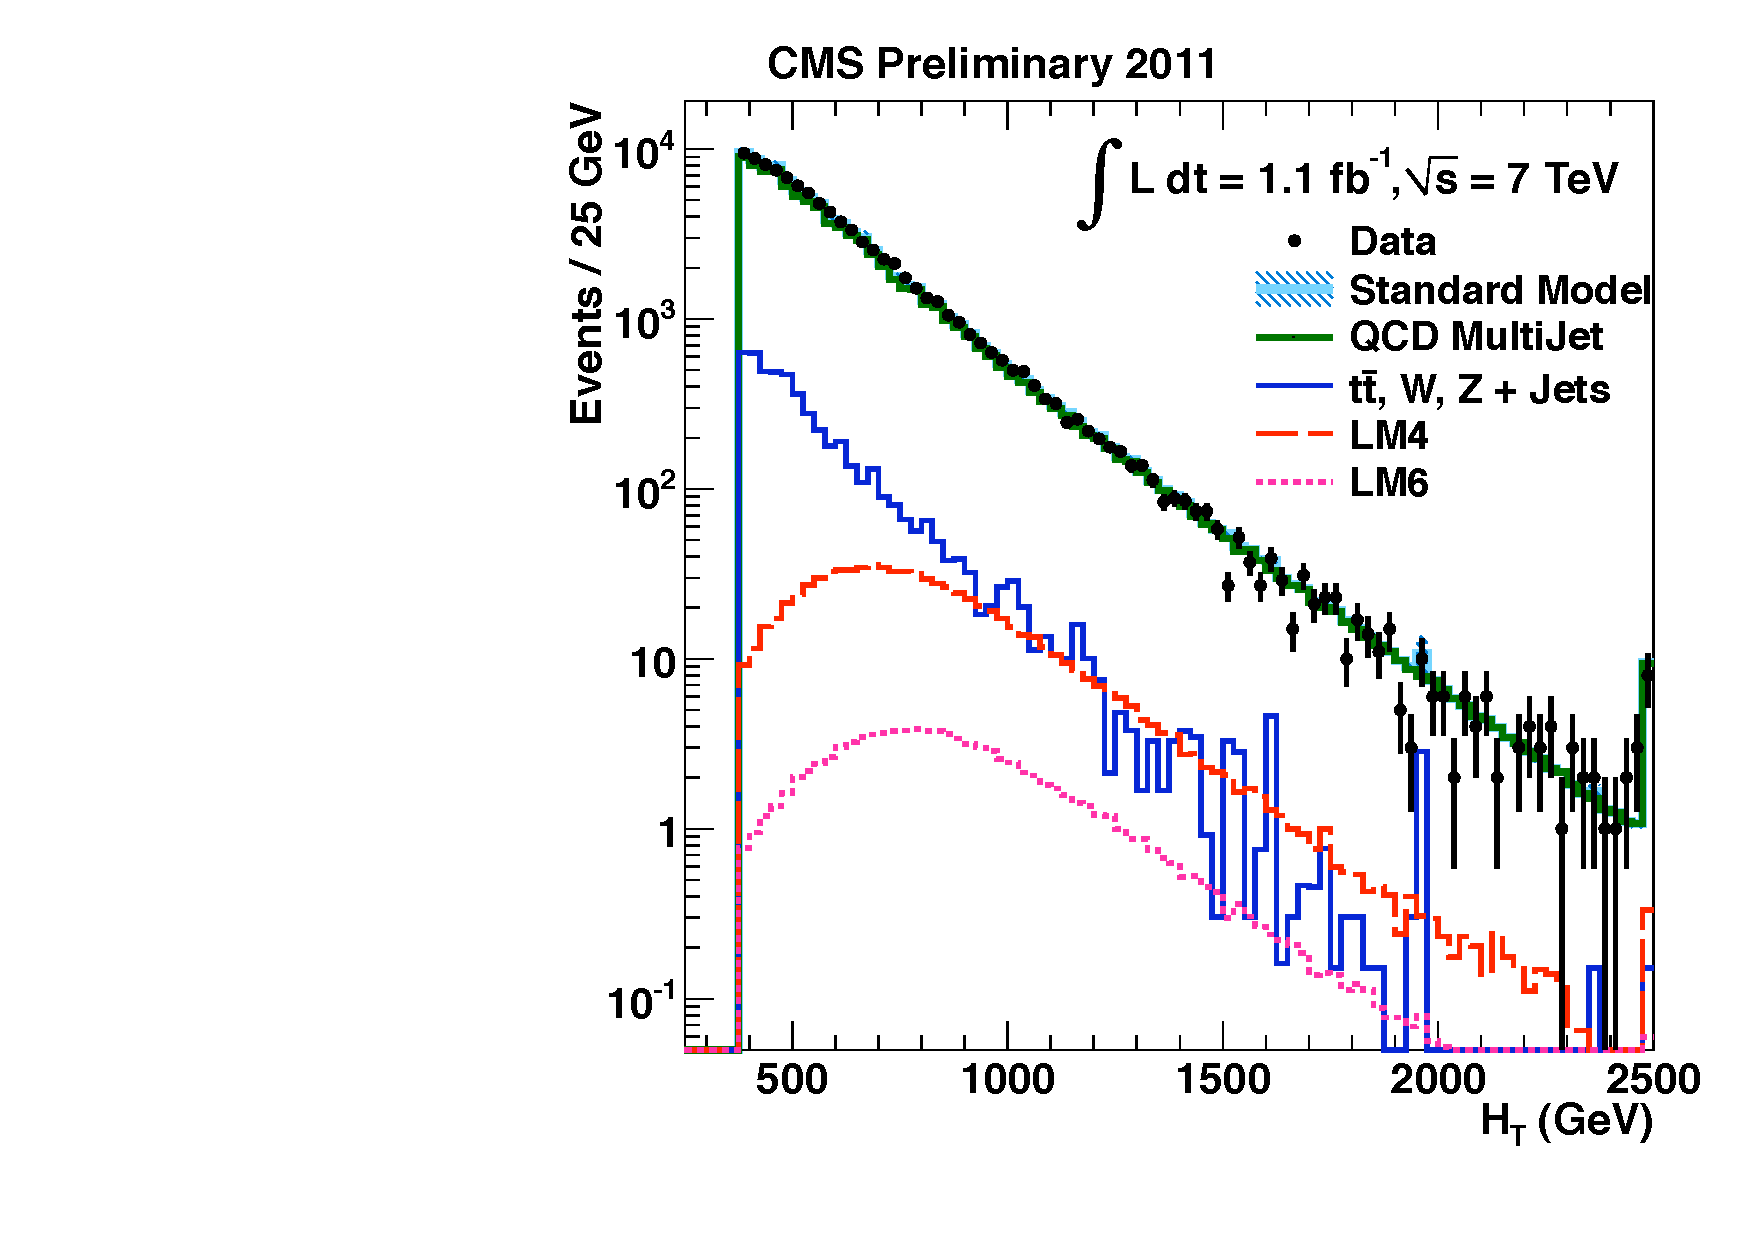
\includegraphics[width=0.45\textwidth]{Figures/Analysis/PAS/HT_all.pdf}}
\hspace{0.2cm}
\subfigure[]{\label{fig:figures_JetMultiplicity_all}
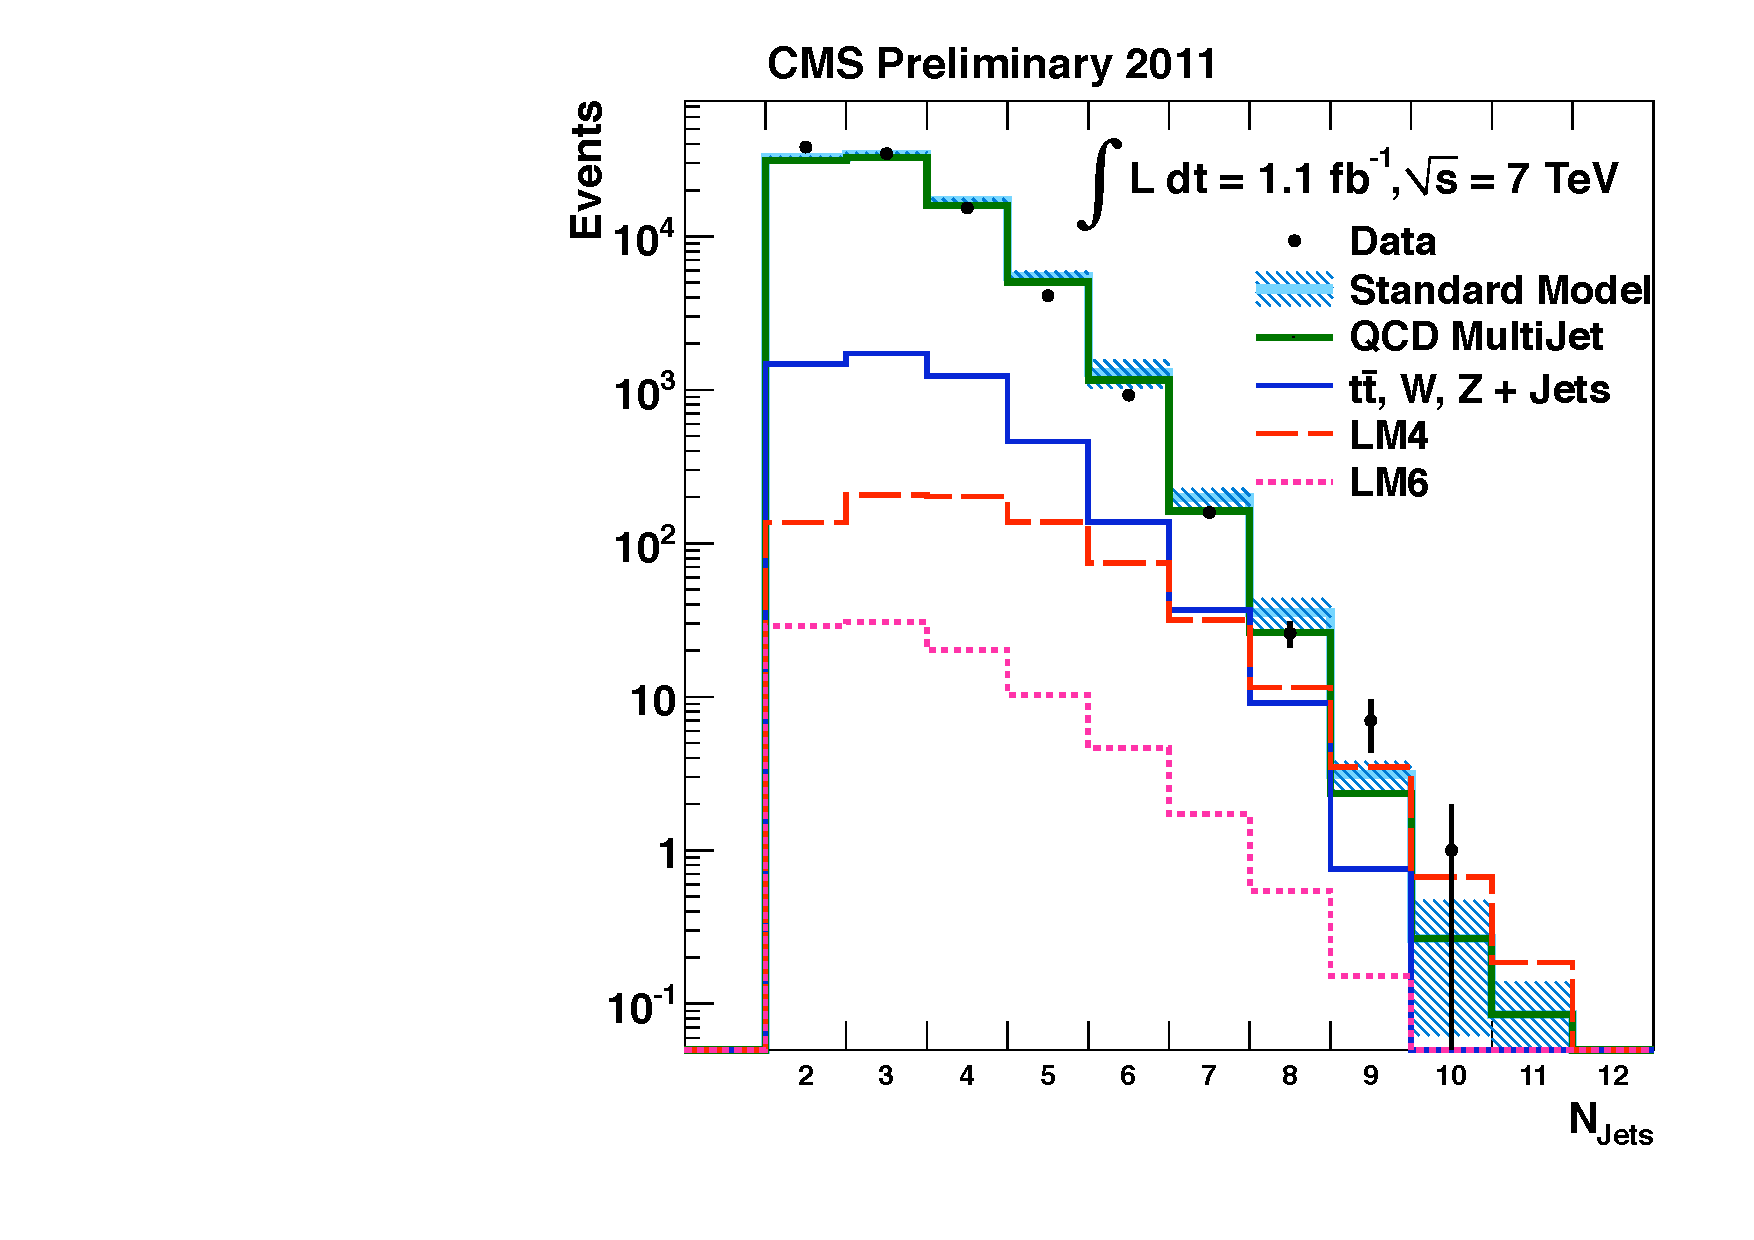
\includegraphics[width=0.45\textwidth]{Figures/Analysis/PAS/JetMultiplicity_all.pdf}
}
\end{minipage}
\newline
\begin{minipage}[b]{1.\textwidth}
\centering
\subfigure[]{\label{fig:figures_AlphaT_all}
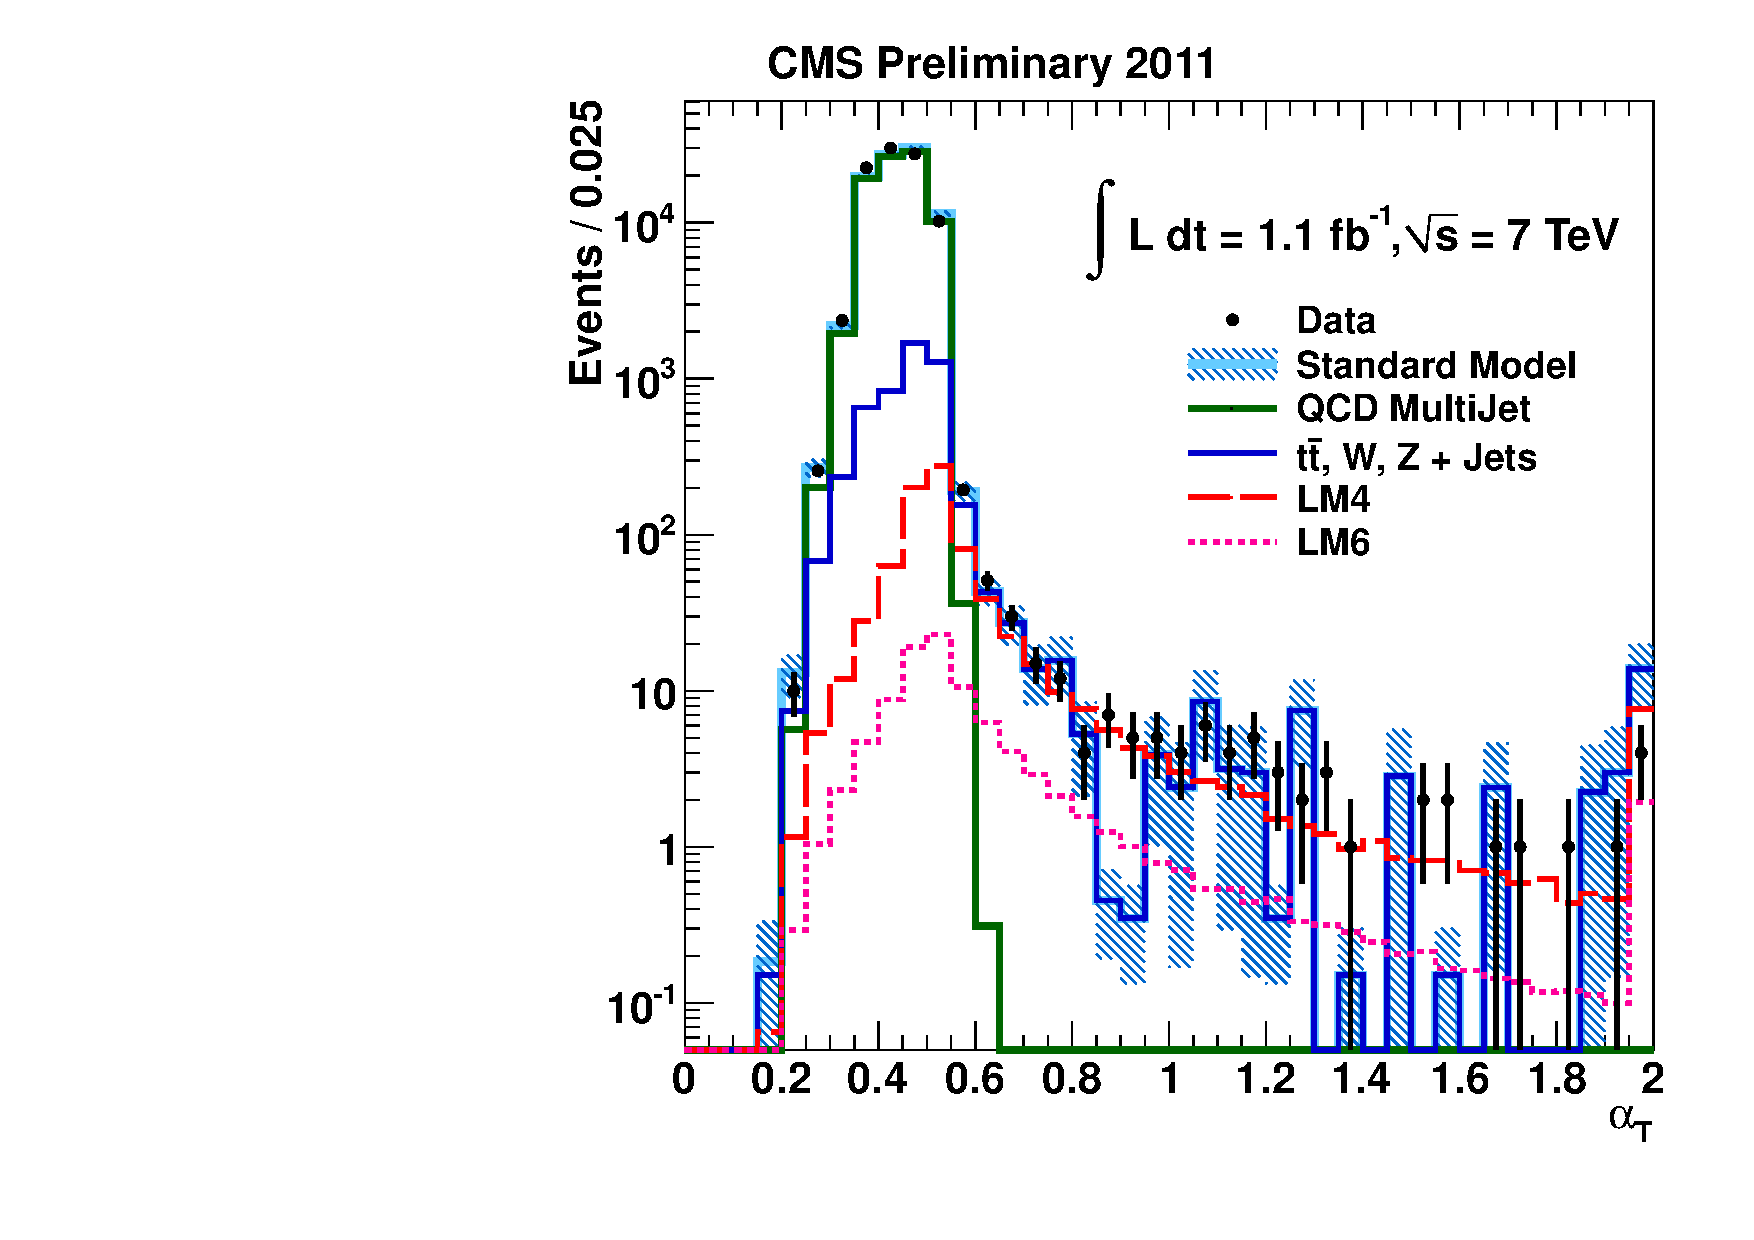
\includegraphics[width=0.45\textwidth]{Figures/Analysis/PAS/AlphaT_all.pdf}
}
\hspace{0.2cm}
  \subfigure[]{\label{fig:figures_AlphaT_Zoomed_all}
          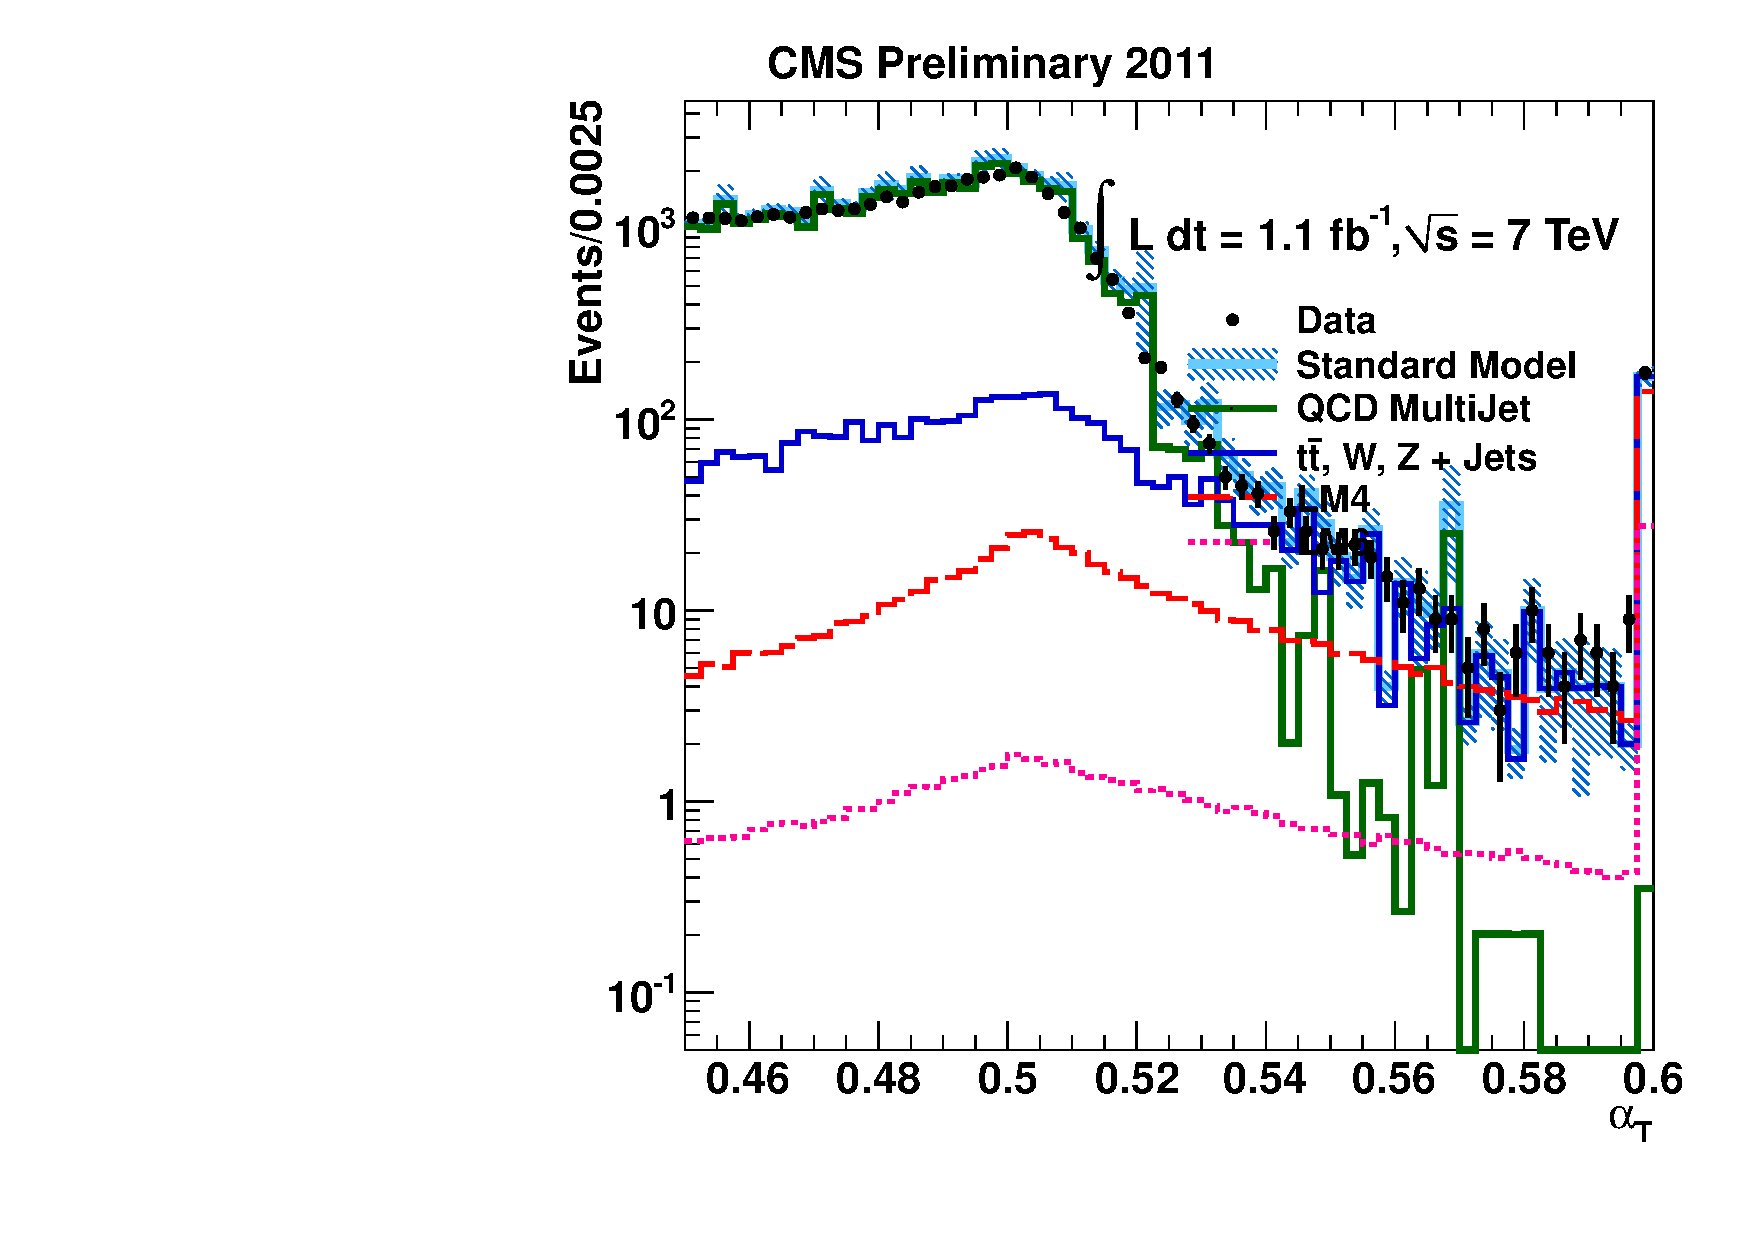
\includegraphics[width=0.45\textwidth]{Figures/Analysis/PAS/AlphaT_Zoomed_all.pdf}
     }
     \end{minipage}
    \caption{\label{fig:preselplot}Distributions of (a) \HT, (b) NJet, (c) \alt showing comparisons of 1.1 \fb 2011 7TeV CMS Data and equivalently weighted Monte-Carlo prior to the $\alpha_{T}$ selection cut, for $\HT \geq 375$~GeV and \MHT $>$ 100~GeV. The \alt distribution is also shown zoomed (d) in the region $0.46 < \alt < 0.6$. SUSY Signal reference points LM4 \& LM6 shown for illustration of potential yields.}
\end{figure}


The distributions of jet multiplicity, $\Delta \phi^{*}$ and $M_{eff}$ after the final selection cuts are applied can be seen respectively in Figure~\ref{afterat}. Data shows a good overall comparison to the Standard Model MC, although here statistics are more limited accounting for fluctuations. The $\Delta \phi^{*}$ distribution in Figure~\ref{fig:fig:BiasedDeltaPhi_after_alphaT_55_all} is consistent with the expectation that the \alt cut completely eradicate contamination from QCD events, as any evidence of such would lead to a peak at low values, instead of the flat behaviour seen. In addition no notable excess can be seen of data over MC although this observation is merely an aside, as a more detailed shape analysis will be used to evaluate this quantitatively in later sections. 

\begin{figure}[htbp]
    \centering
     \subfigure[]{
          \label{fig:JetMultiplicityAfterAlphaT_all}
          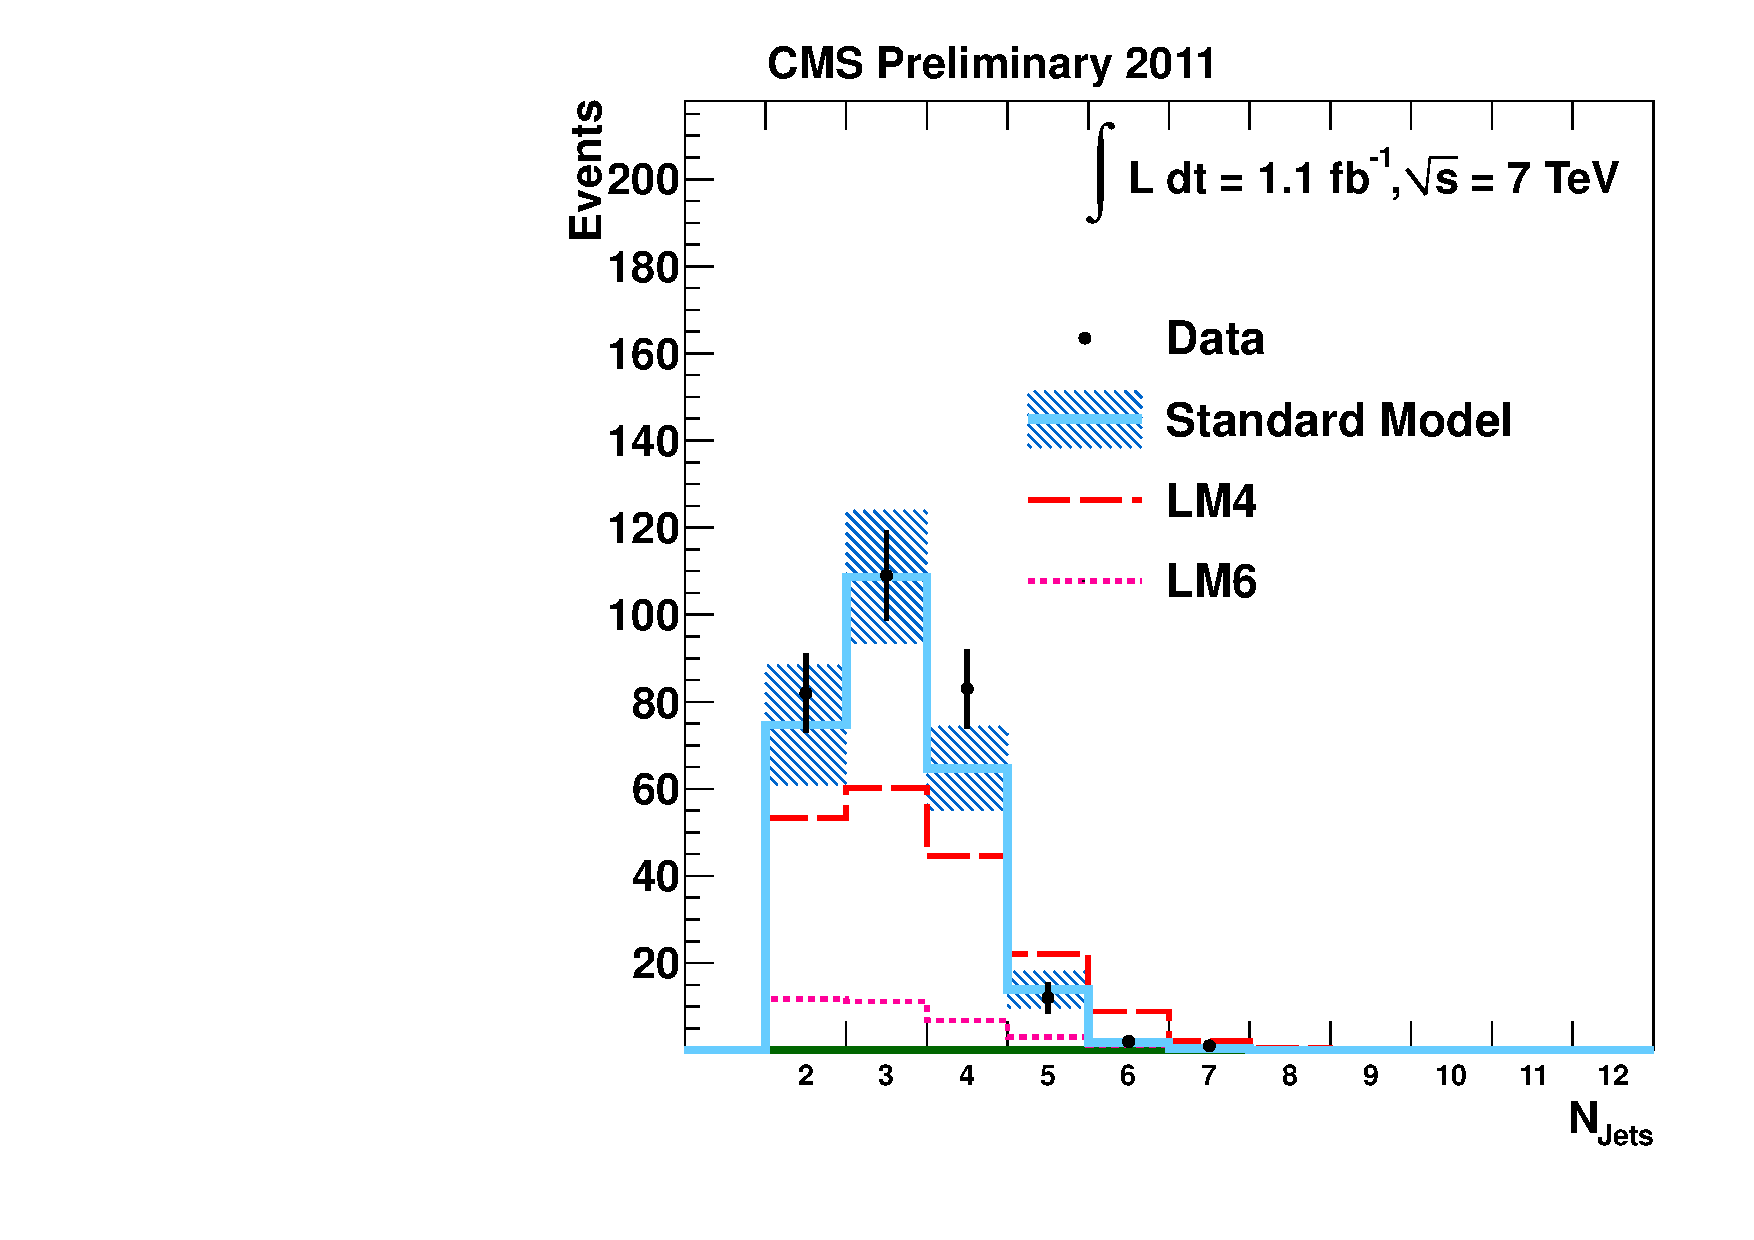
\includegraphics[width=0.45\textwidth]{Figures/Analysis/PAS/JetMultiplicityAfterAlphaT_all.pdf}
     }
    \subfigure[]{
          \label{fig:EffectiveMass_after_alphaT_55_all}
          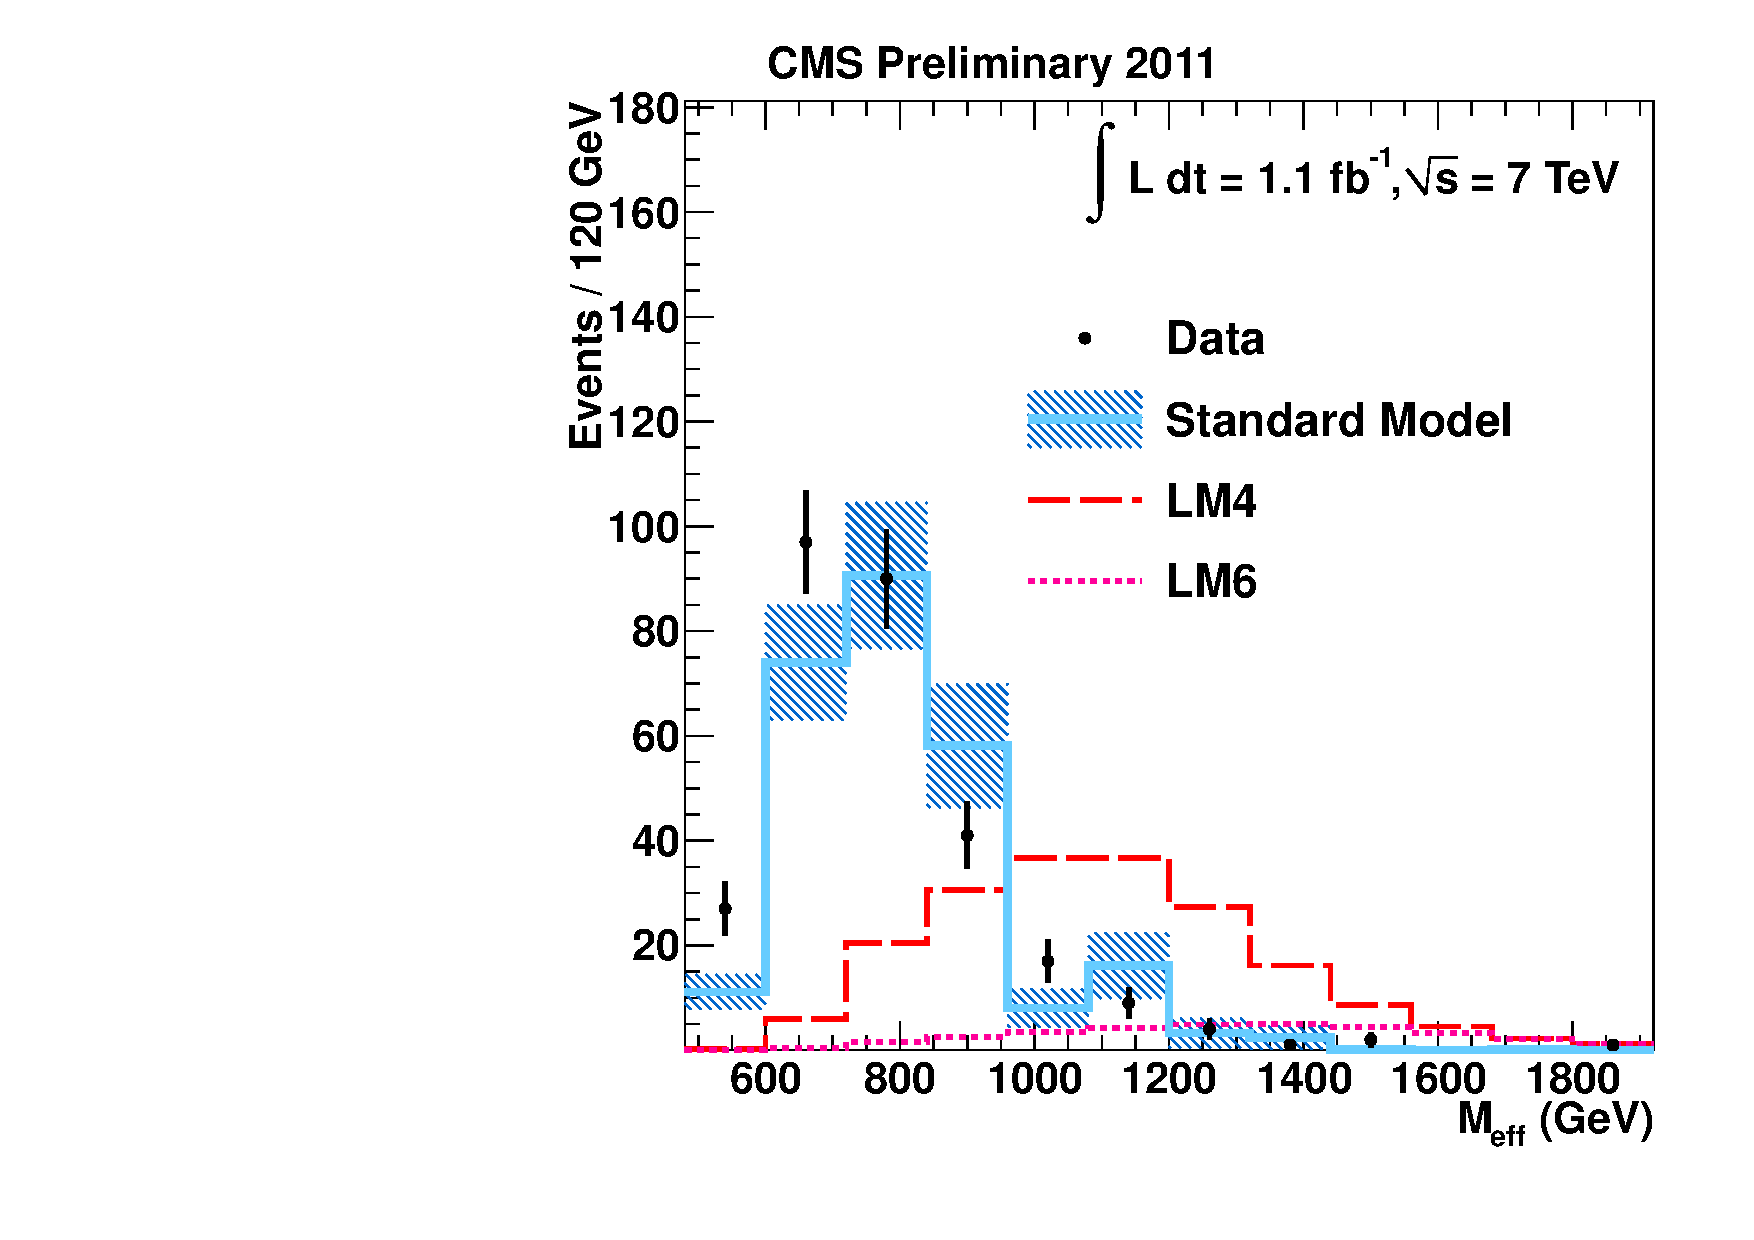
\includegraphics[width=0.45\textwidth]{Figures/Analysis/PAS/EffectiveMass_after_alphaT_55_all.pdf}
     }
     \newline
     \subfigure[]{
          \label{fig:BiasedDeltaPhi_after_alphaT_55_all}
          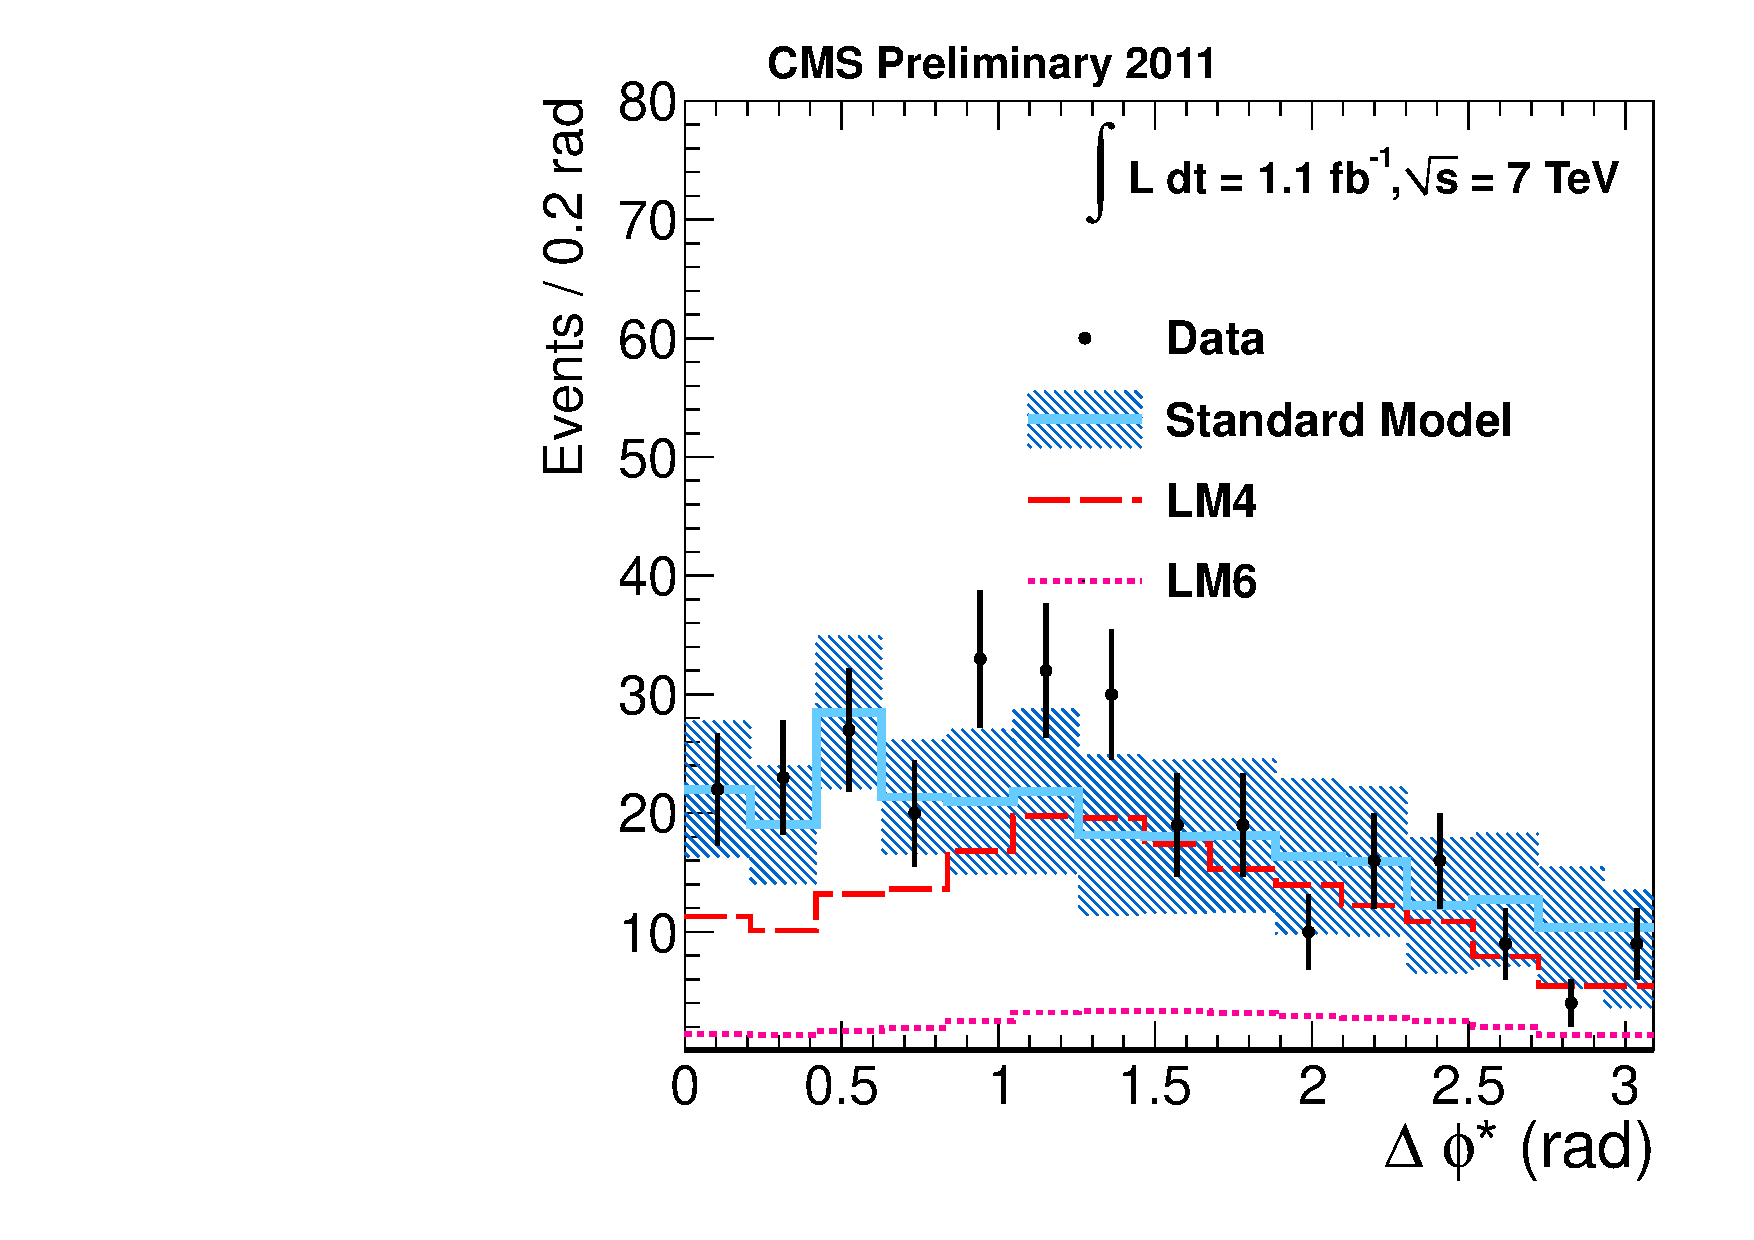
\includegraphics[width=0.45\textwidth]{Figures/Analysis/PAS/BiasedDeltaPhi_after_alphaT_55_all.pdf}
     }

   
\caption{\label{fig:after at}Distributions of (a) Jet Multiplicity, (b) $M_{\rm eff}$( = $H_{T}$ + \MHT) and (c) $\Delta \phi^{*}$ showing comparisons of 1.1 \fb 2011 7TeV CMS Data and equivalently weighted Standard Model Monte-Carlo in basic kinematic quantities after the full $\alpha_{T}$ selection. SUSY Signal reference points LM4 \& LM6 shown for illustration of potential yields.}
\end{figure}

\subsection{Dependence of $R_{\alpha_{T}}$ on $H_{T}$}




\begin{figure}[h]
  \begin{center}
    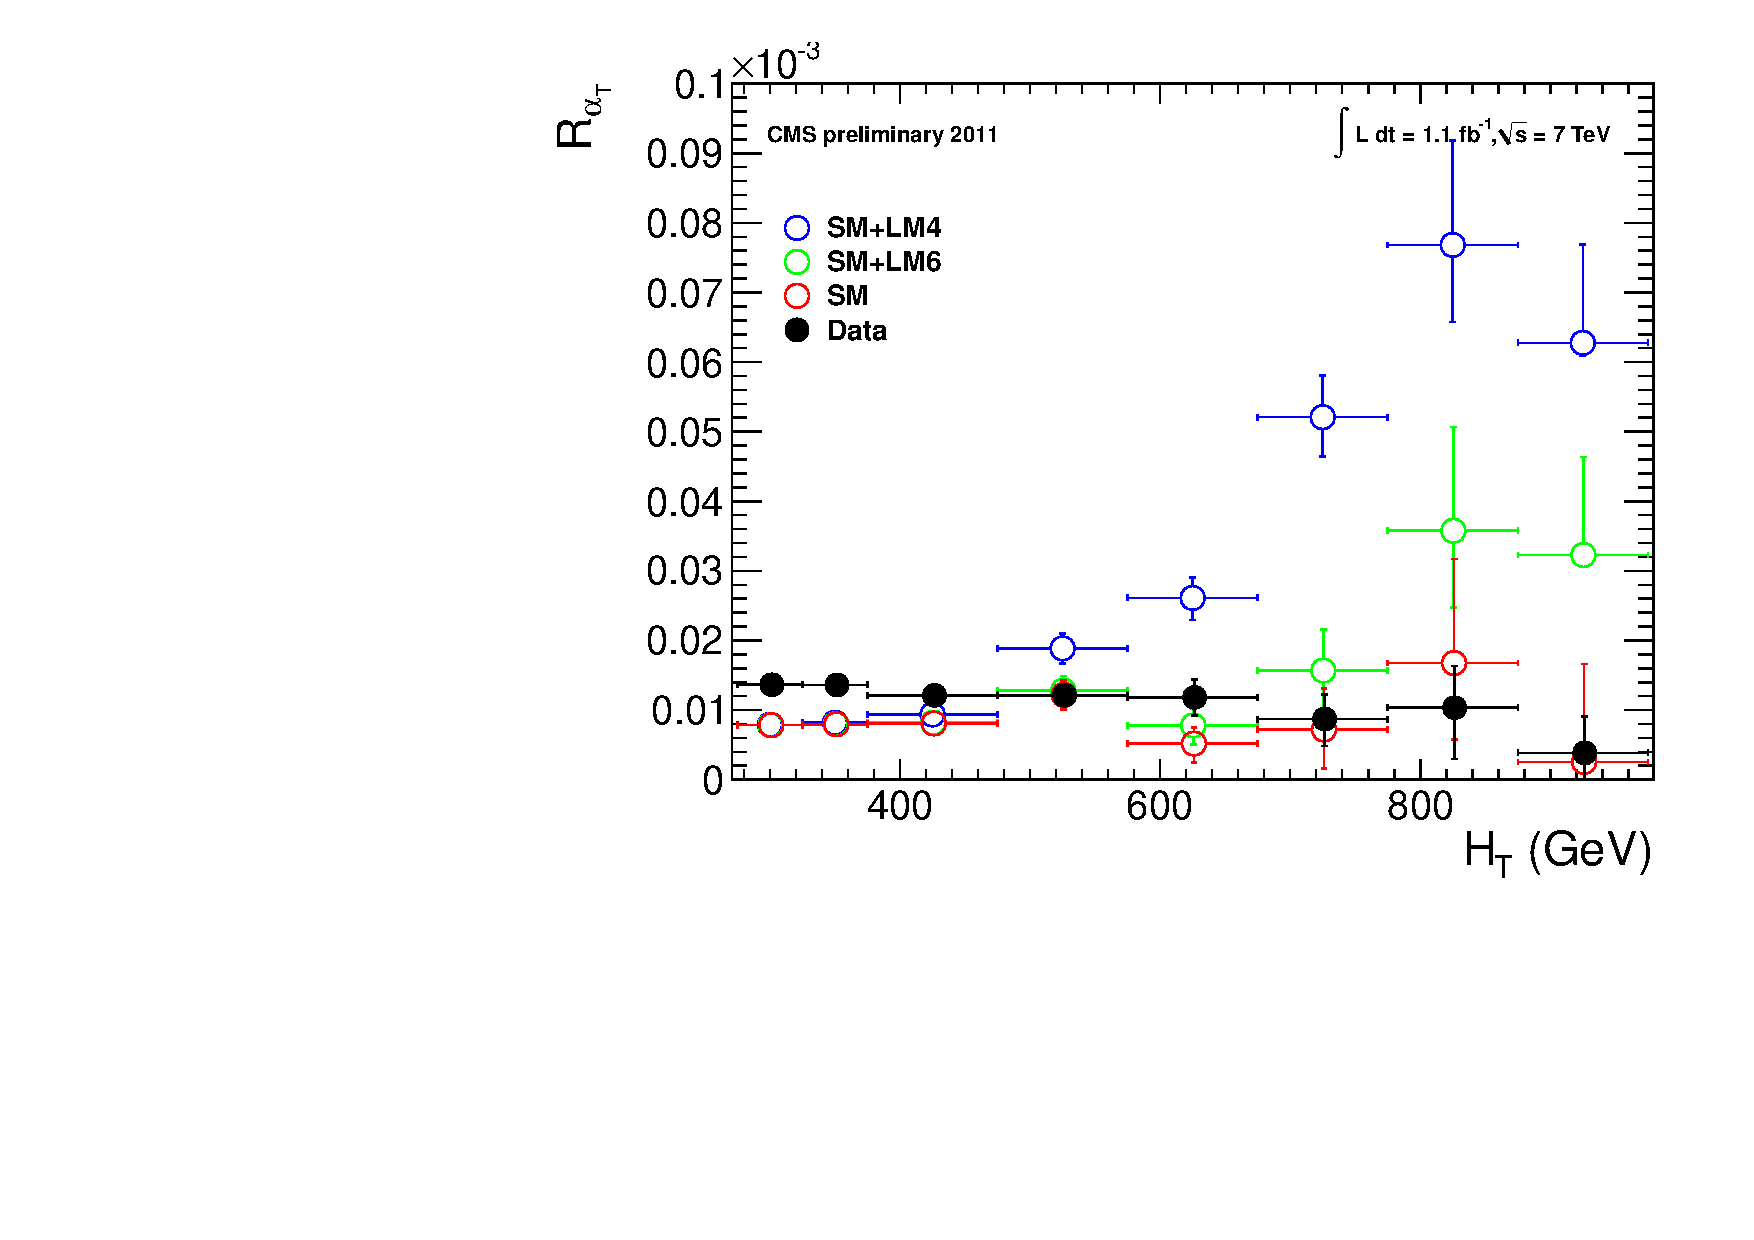
\includegraphics[width = 0.48\textwidth]{Figures/Analysis/PAS/Ratio_Multi2Incl_AlphaT55.pdf}
    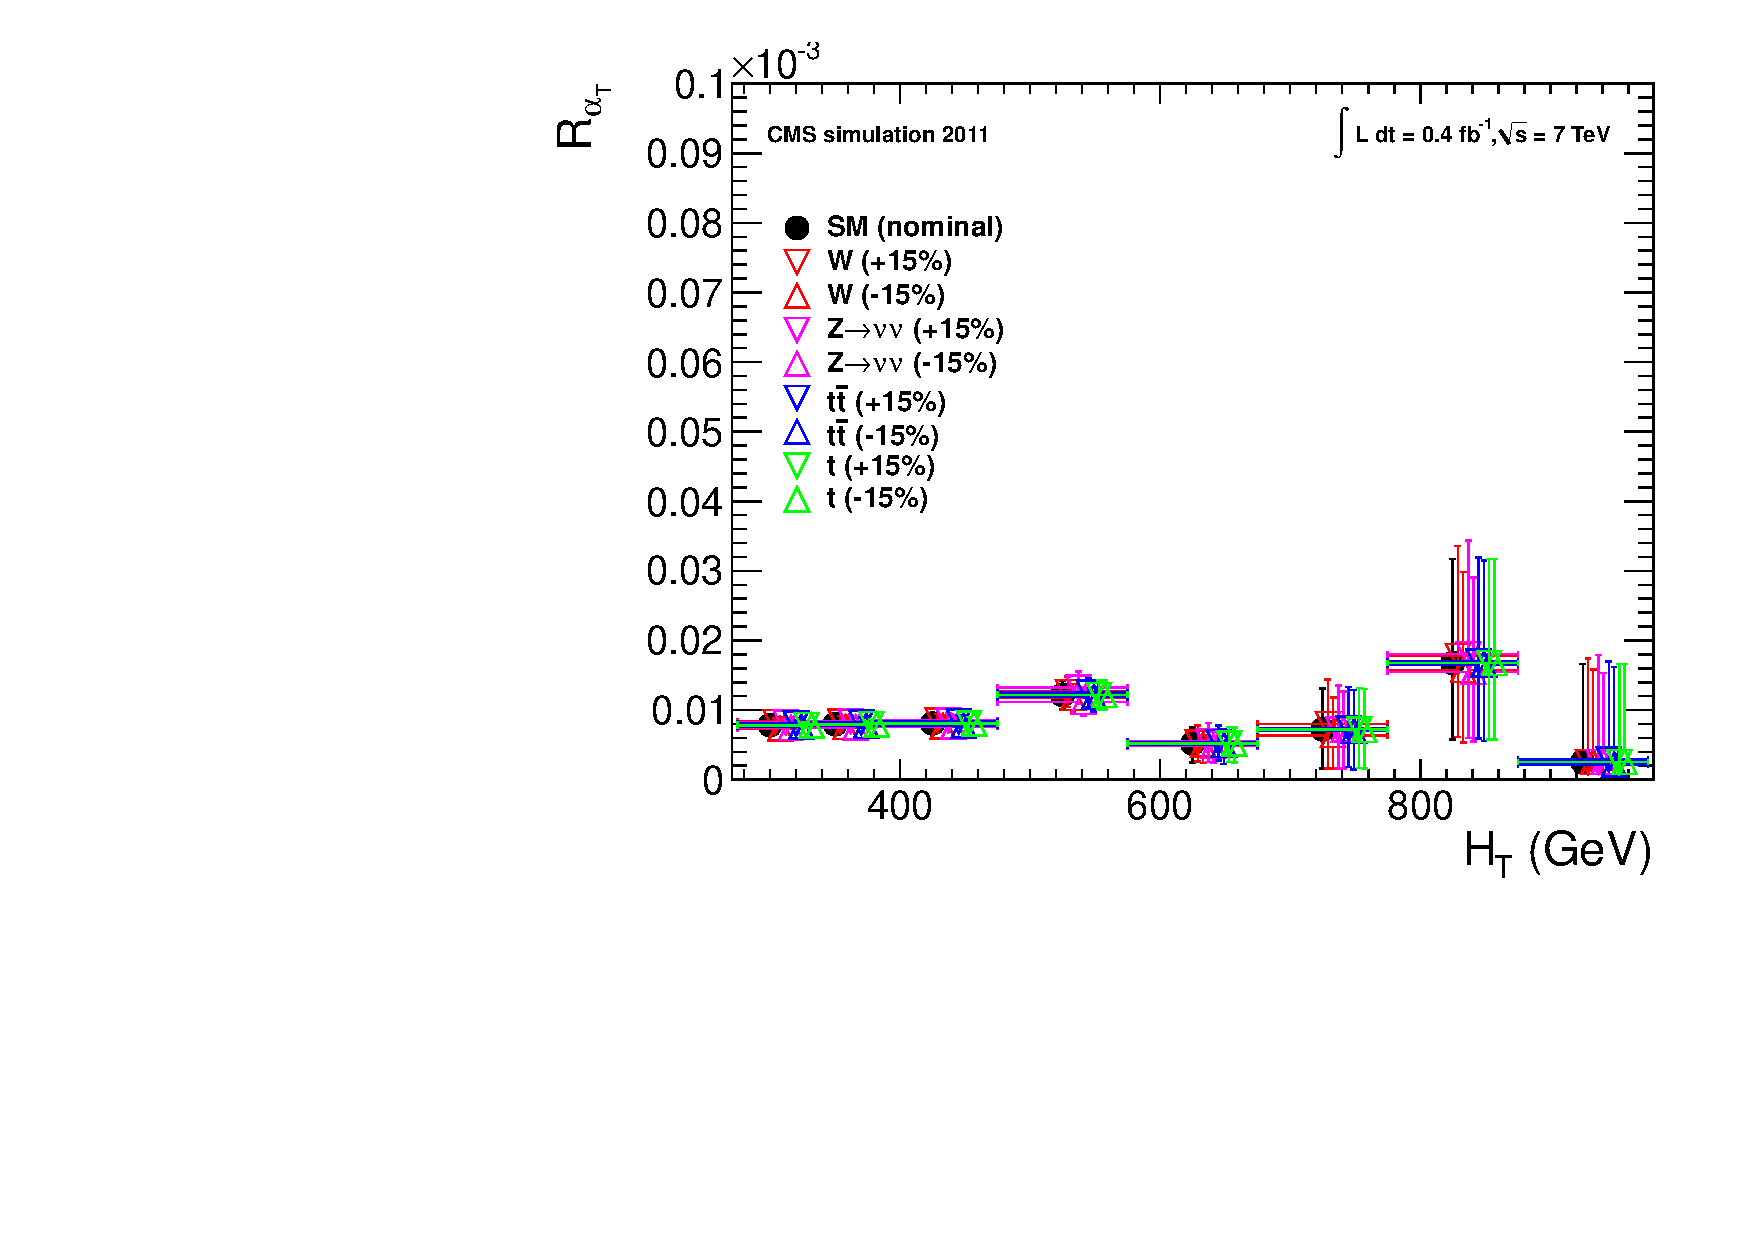
\includegraphics[width = 0.48\textwidth]{Figures/Analysis/PAS/Syst_Multi2Incl_AlphaT55.pdf}
    \caption{\label{fig:rat_vs_ht} (Left) The dependence of \RaT on
      \HT for events with N$_{\mathrm{jet}} \geq 2$. (Right) Dependence of rat on
      \HT when varying the effective cross-section of the four major
      EWK background components individually by $\pm$15\%. (Markers
      are artificially offset for clarity.)  }
  \end{center}
\end{figure}






\section{Data-Driven Background Estimation}
\subsection{Total background prediction}
\subsection{Estimating EWK background using high $p_{T}$ using W+Jets events}
\begin{figure}[h]
\begin{center}
\subfigure[\label{fig:muon_beforeat_mupt}]{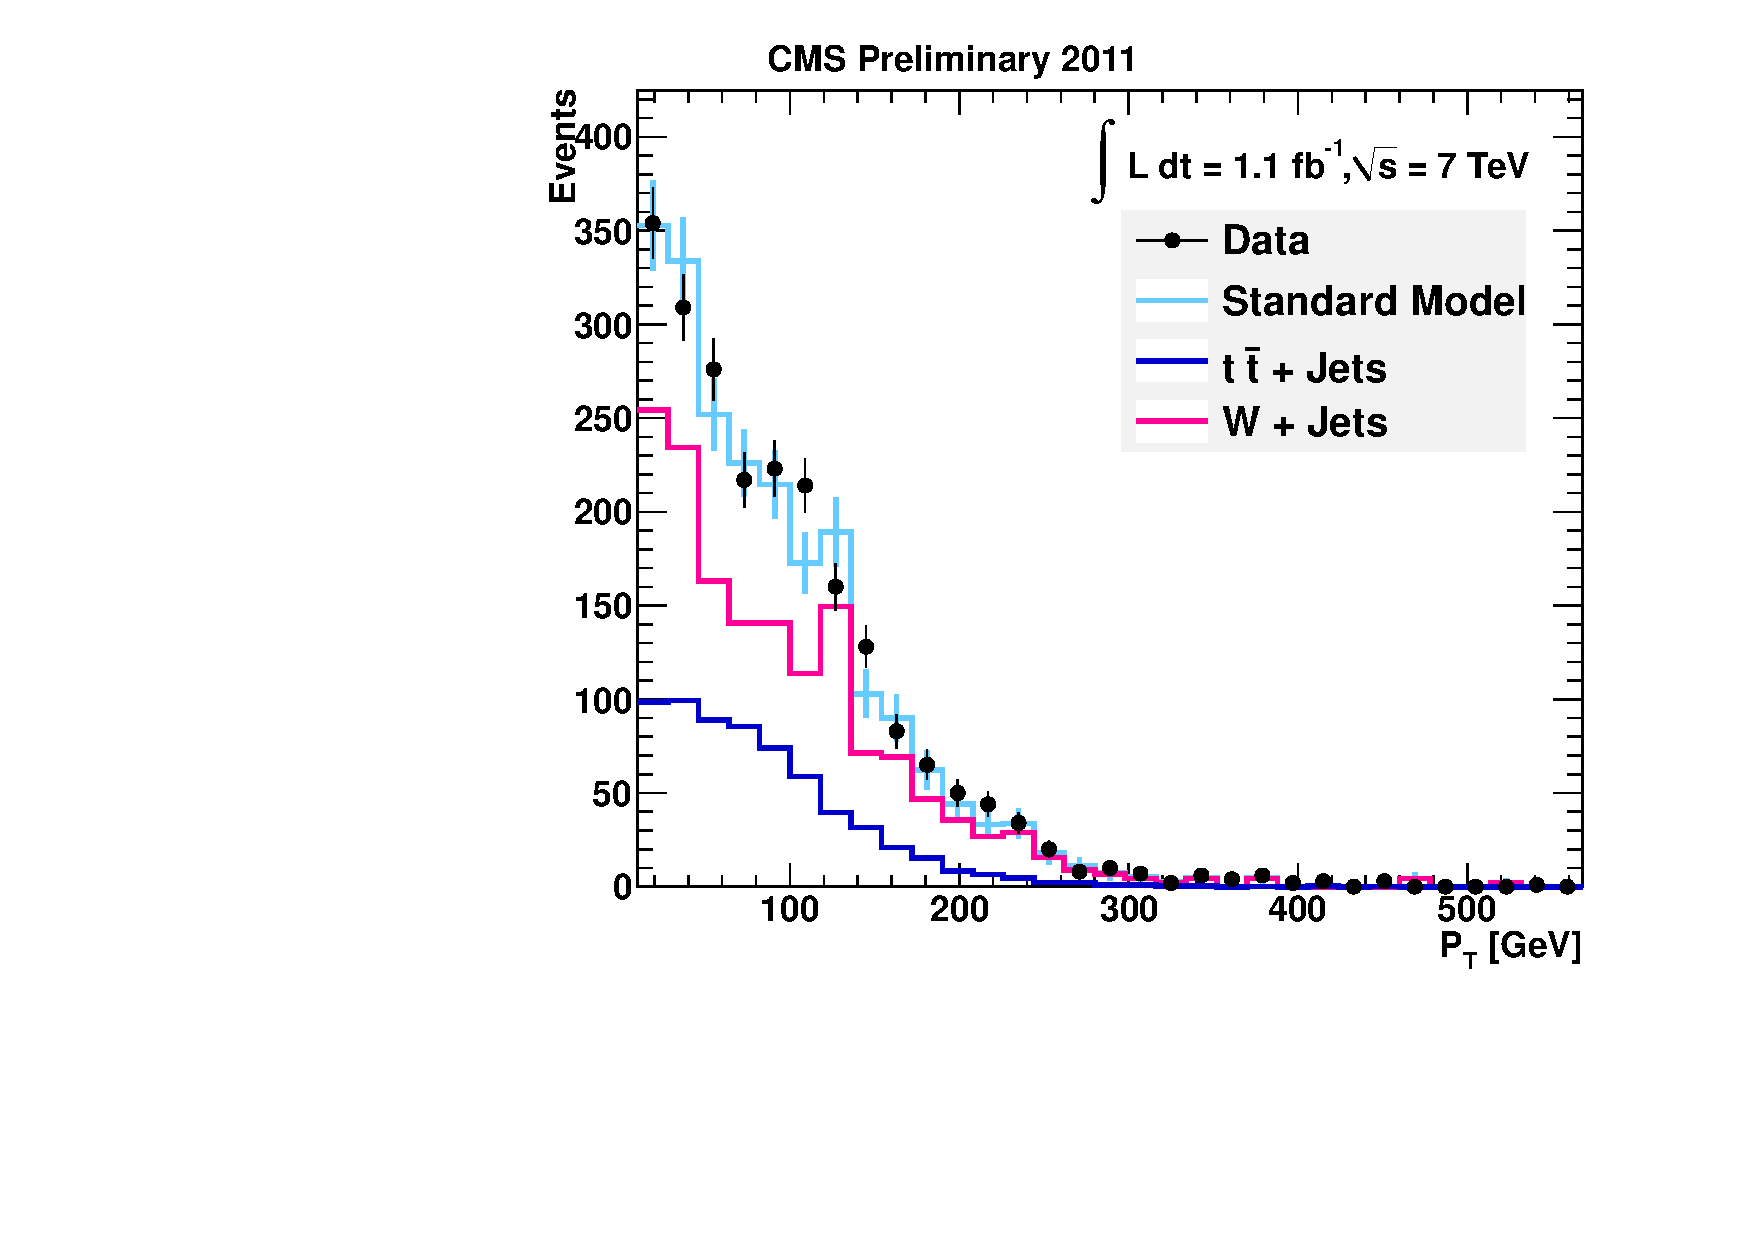
\includegraphics[width=0.45\textwidth, angle=0]{Figures/Analysis/PAS/muon_plots/spring11NoLogYMuPtMuonControl_beforeaT.pdf}}
\subfigure[\label{fig:muon_beforeat_njet}]{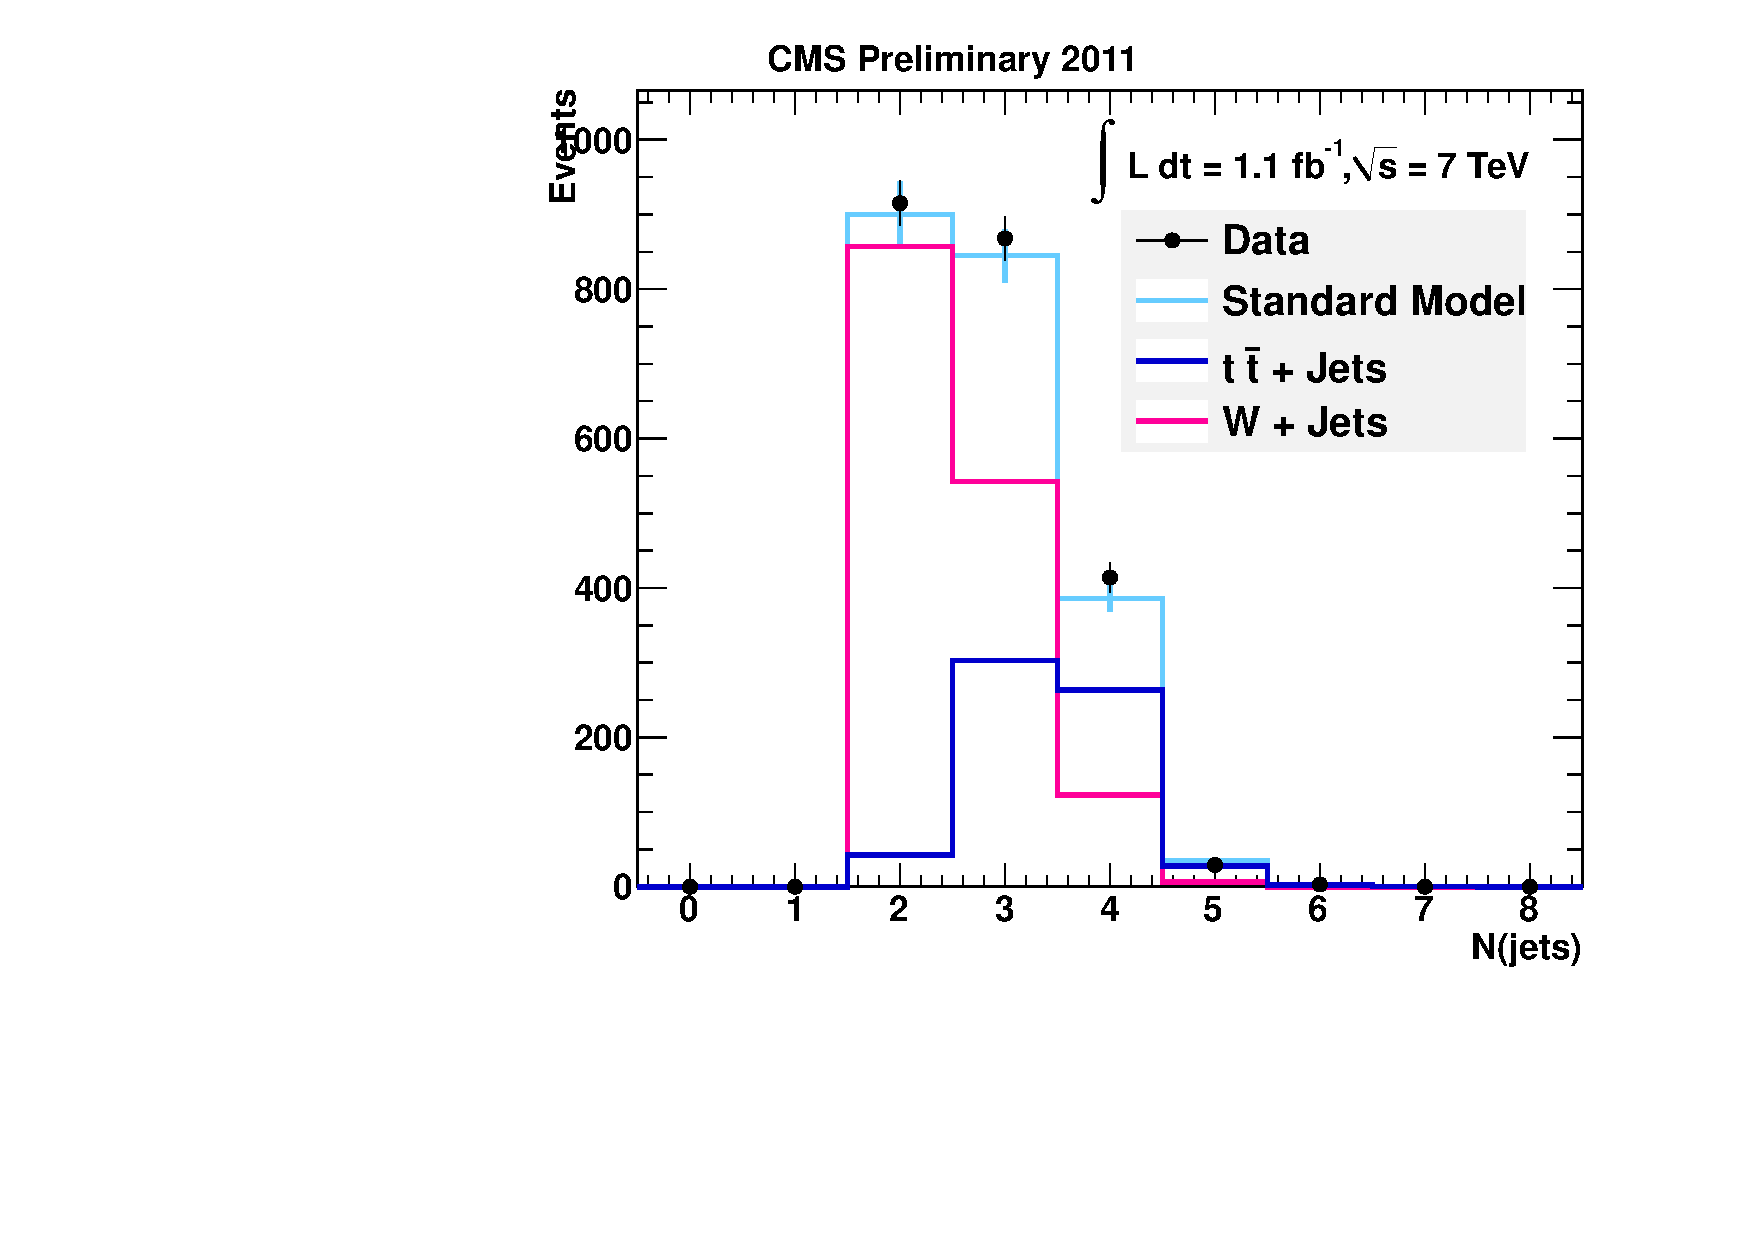
\includegraphics[width=0.45\textwidth, angle=0]{Figures/Analysis/PAS/muon_plots/spring11NoLogYnJetMuonControl_beforeaT.pdf}}
\newline
\subfigure[\label{fig:muon_beforeat_at}]{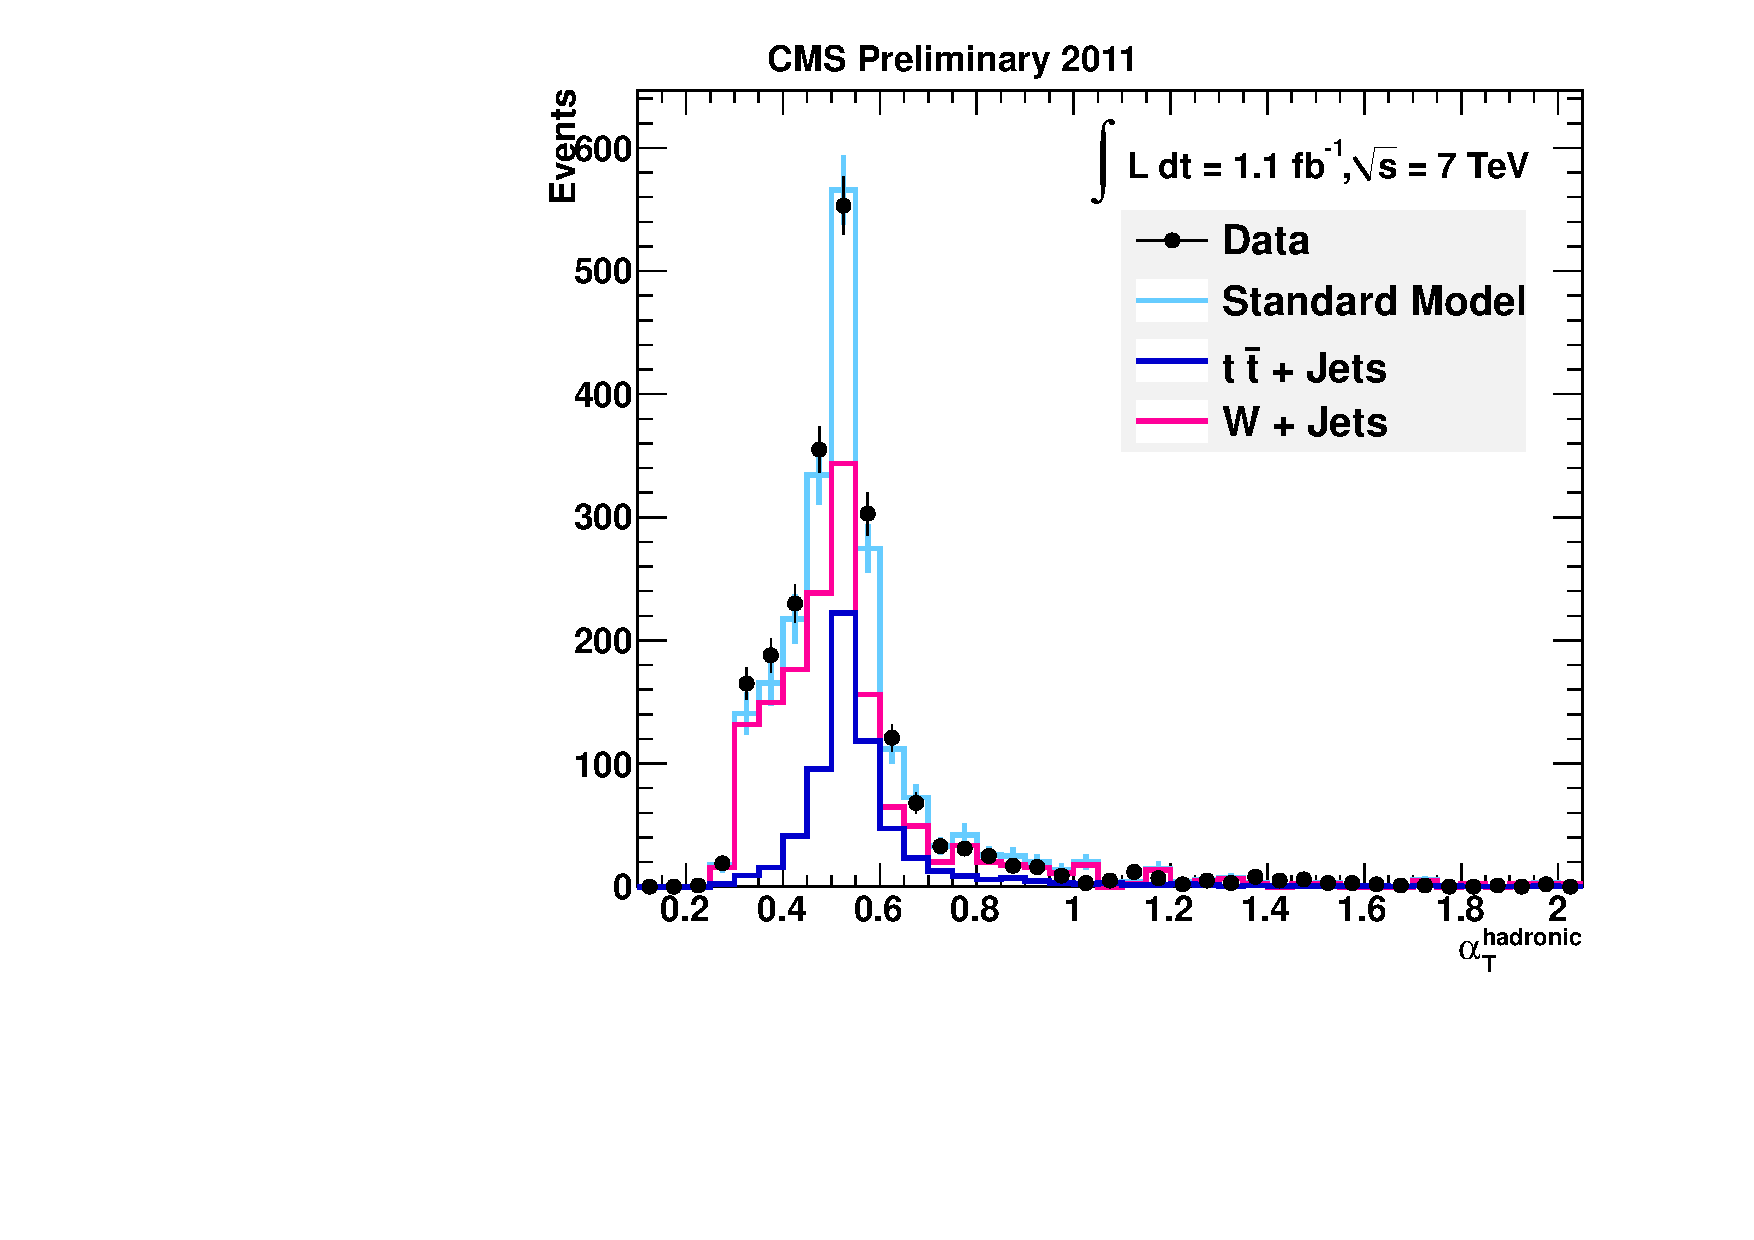
\includegraphics[width=0.45\textwidth, angle=0]{Figures/Analysis/PAS/muon_plots/spring11NoLogYaT_HMuonControl_beforeaT.pdf}}
\subfigure[\label{fig:muon_beforeat_ht}]{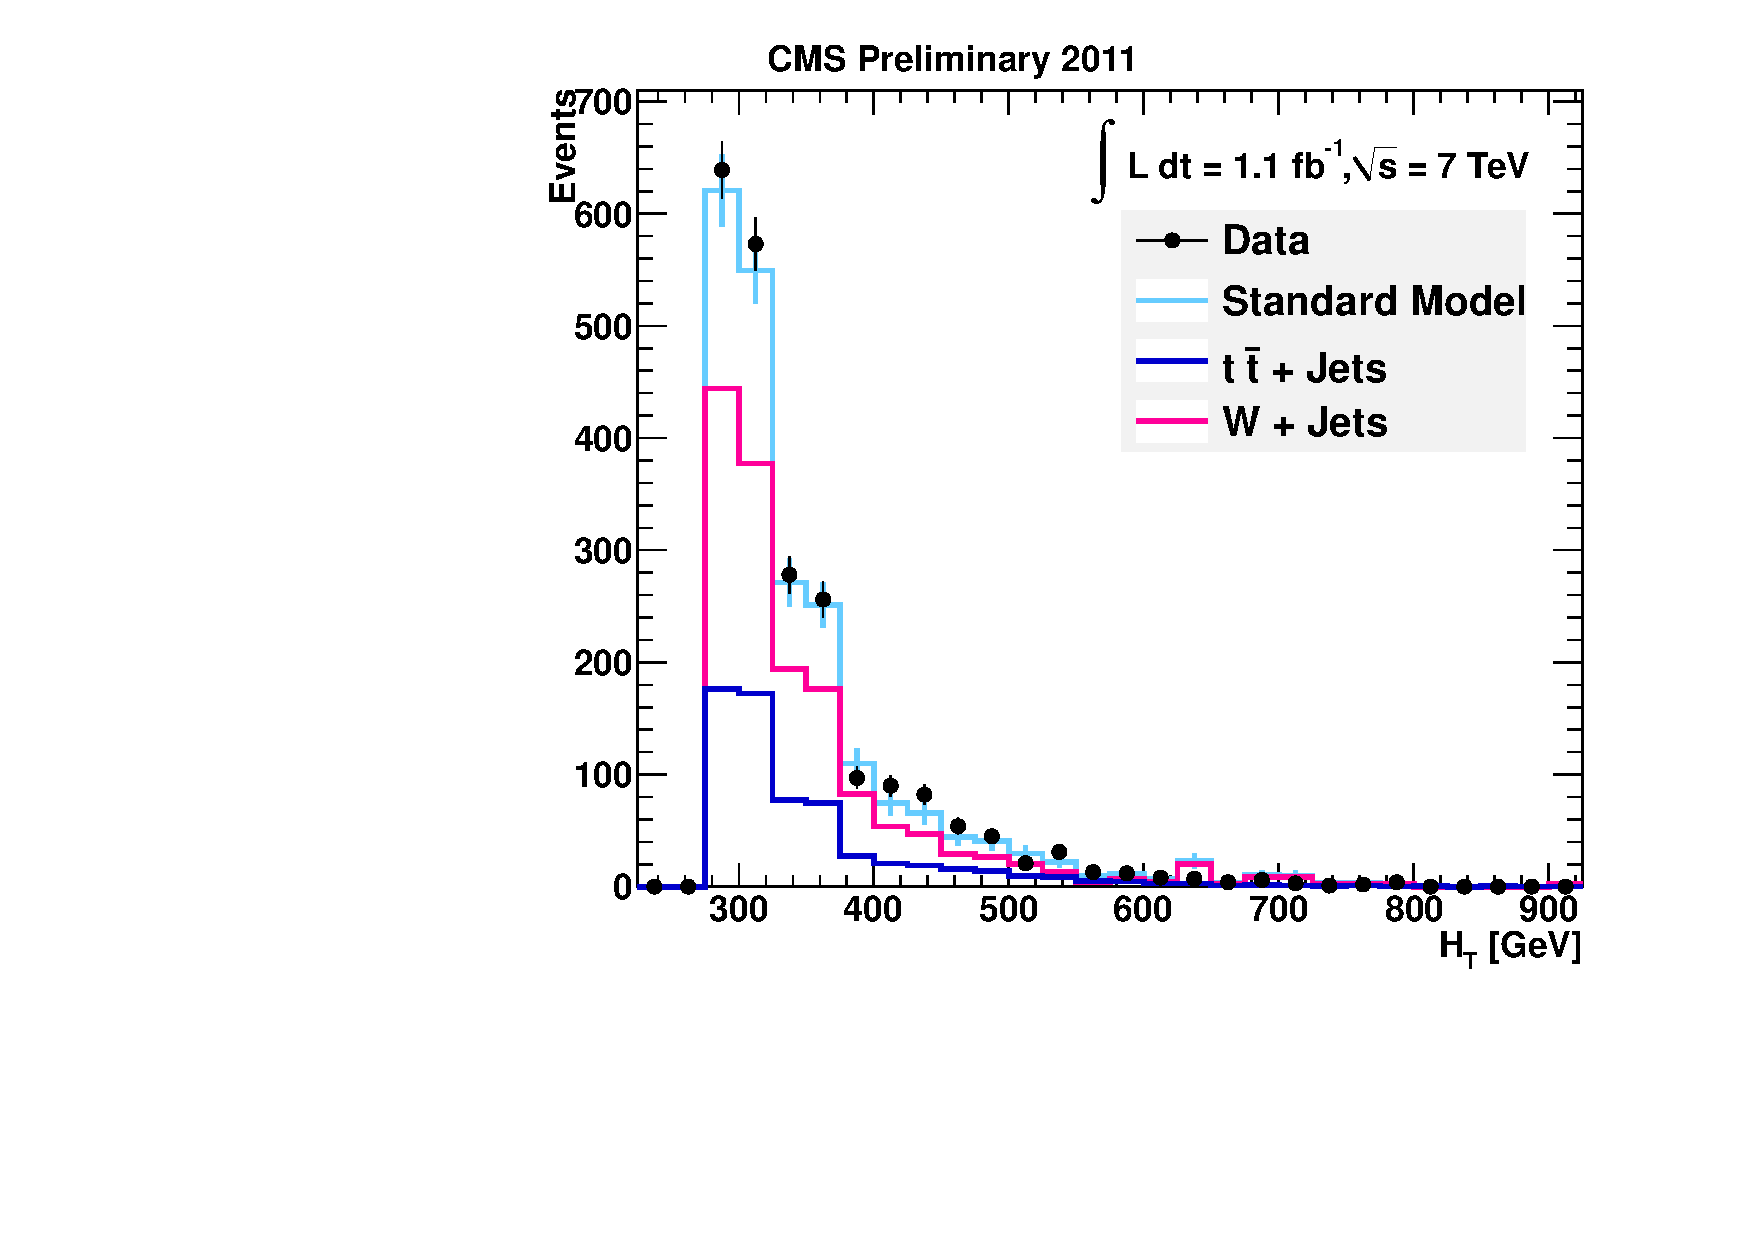
\includegraphics[width=0.45\textwidth, angle=0]{Figures/Analysis/PAS/muon_plots/spring11NoLogYHTMuonControl_beforeaT.pdf}}
\newline
\subfigure[\label{fig:muon_beforeat_MuIso}]{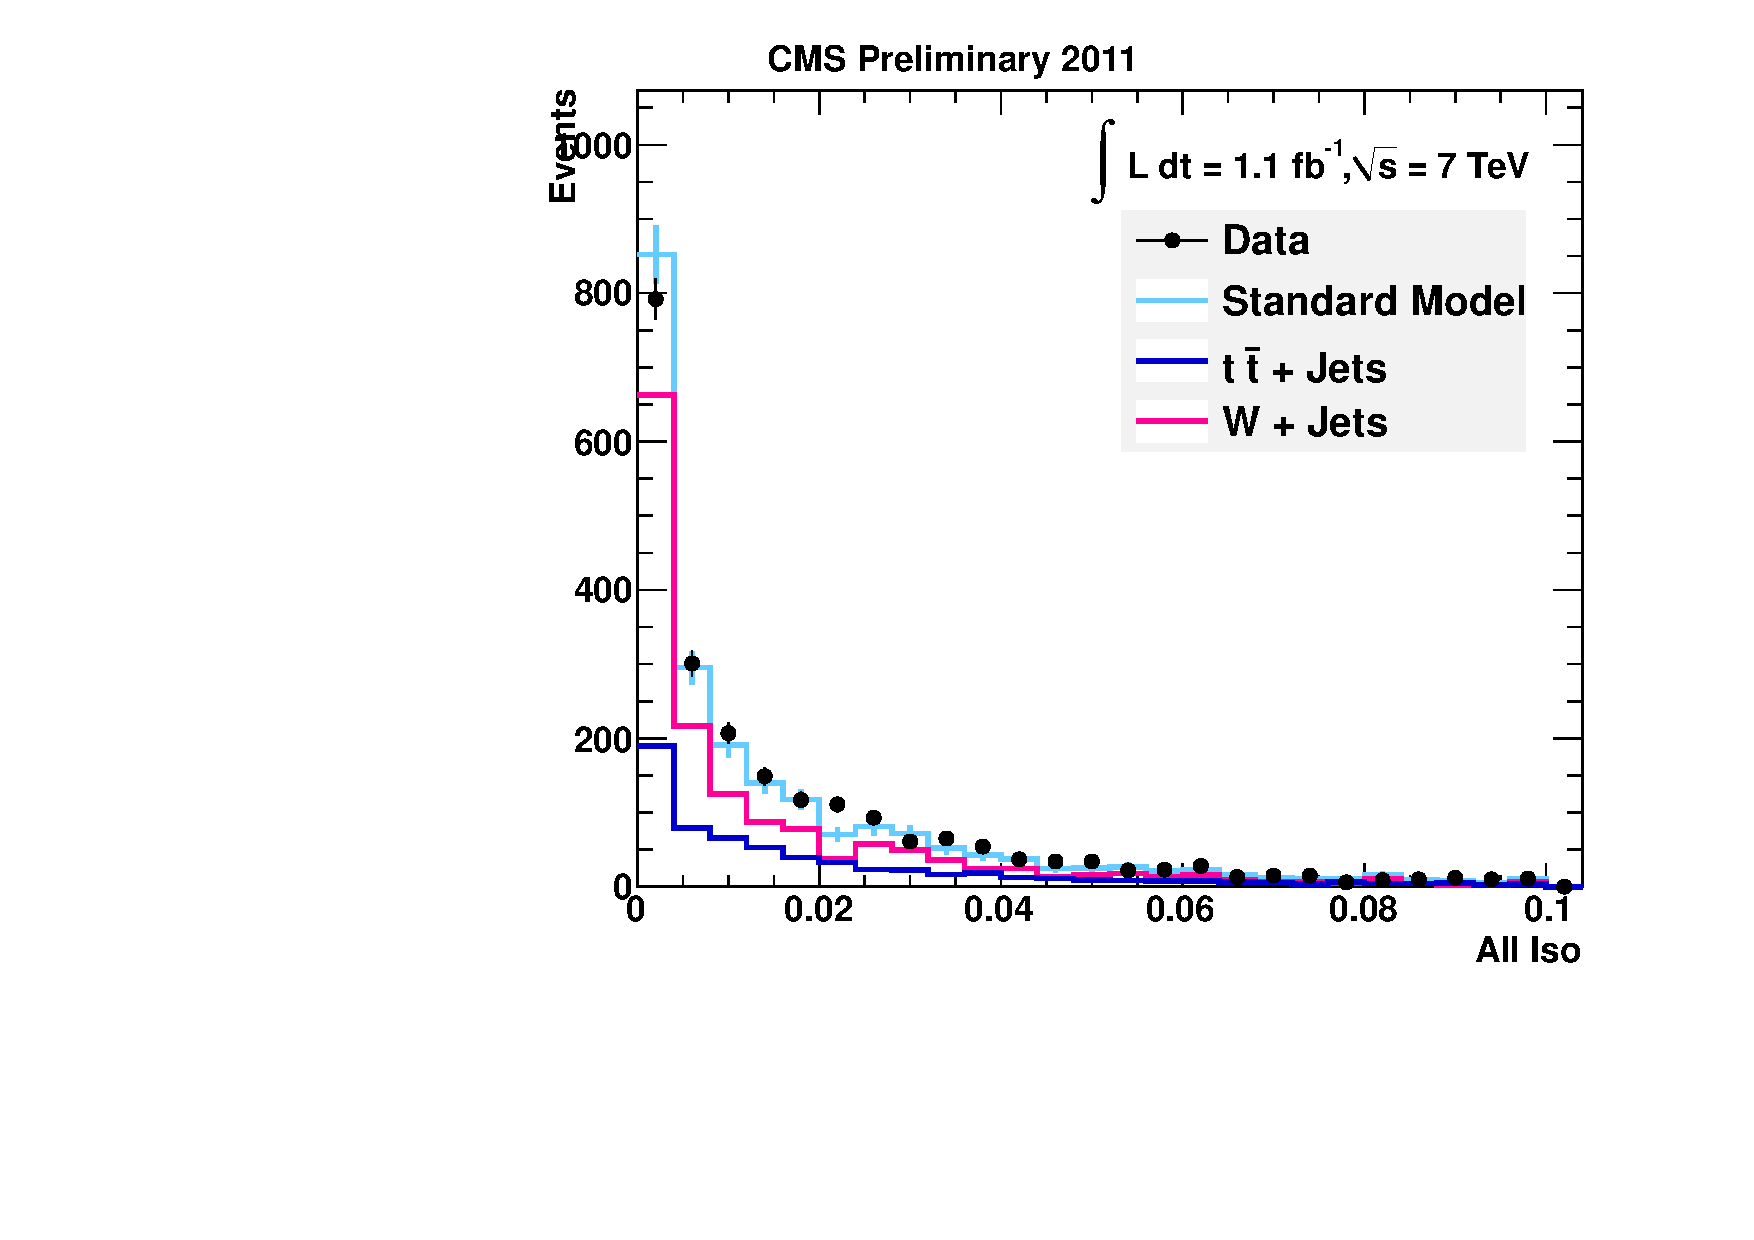
\includegraphics[width=0.45\textwidth, angle=0]{Figures/Analysis/PAS/muon_plots/spring11NoLogYMuCsoMuonControl_beforeaT.pdf}}
\subfigure[\label{fig:muon_beforeat_mt}]{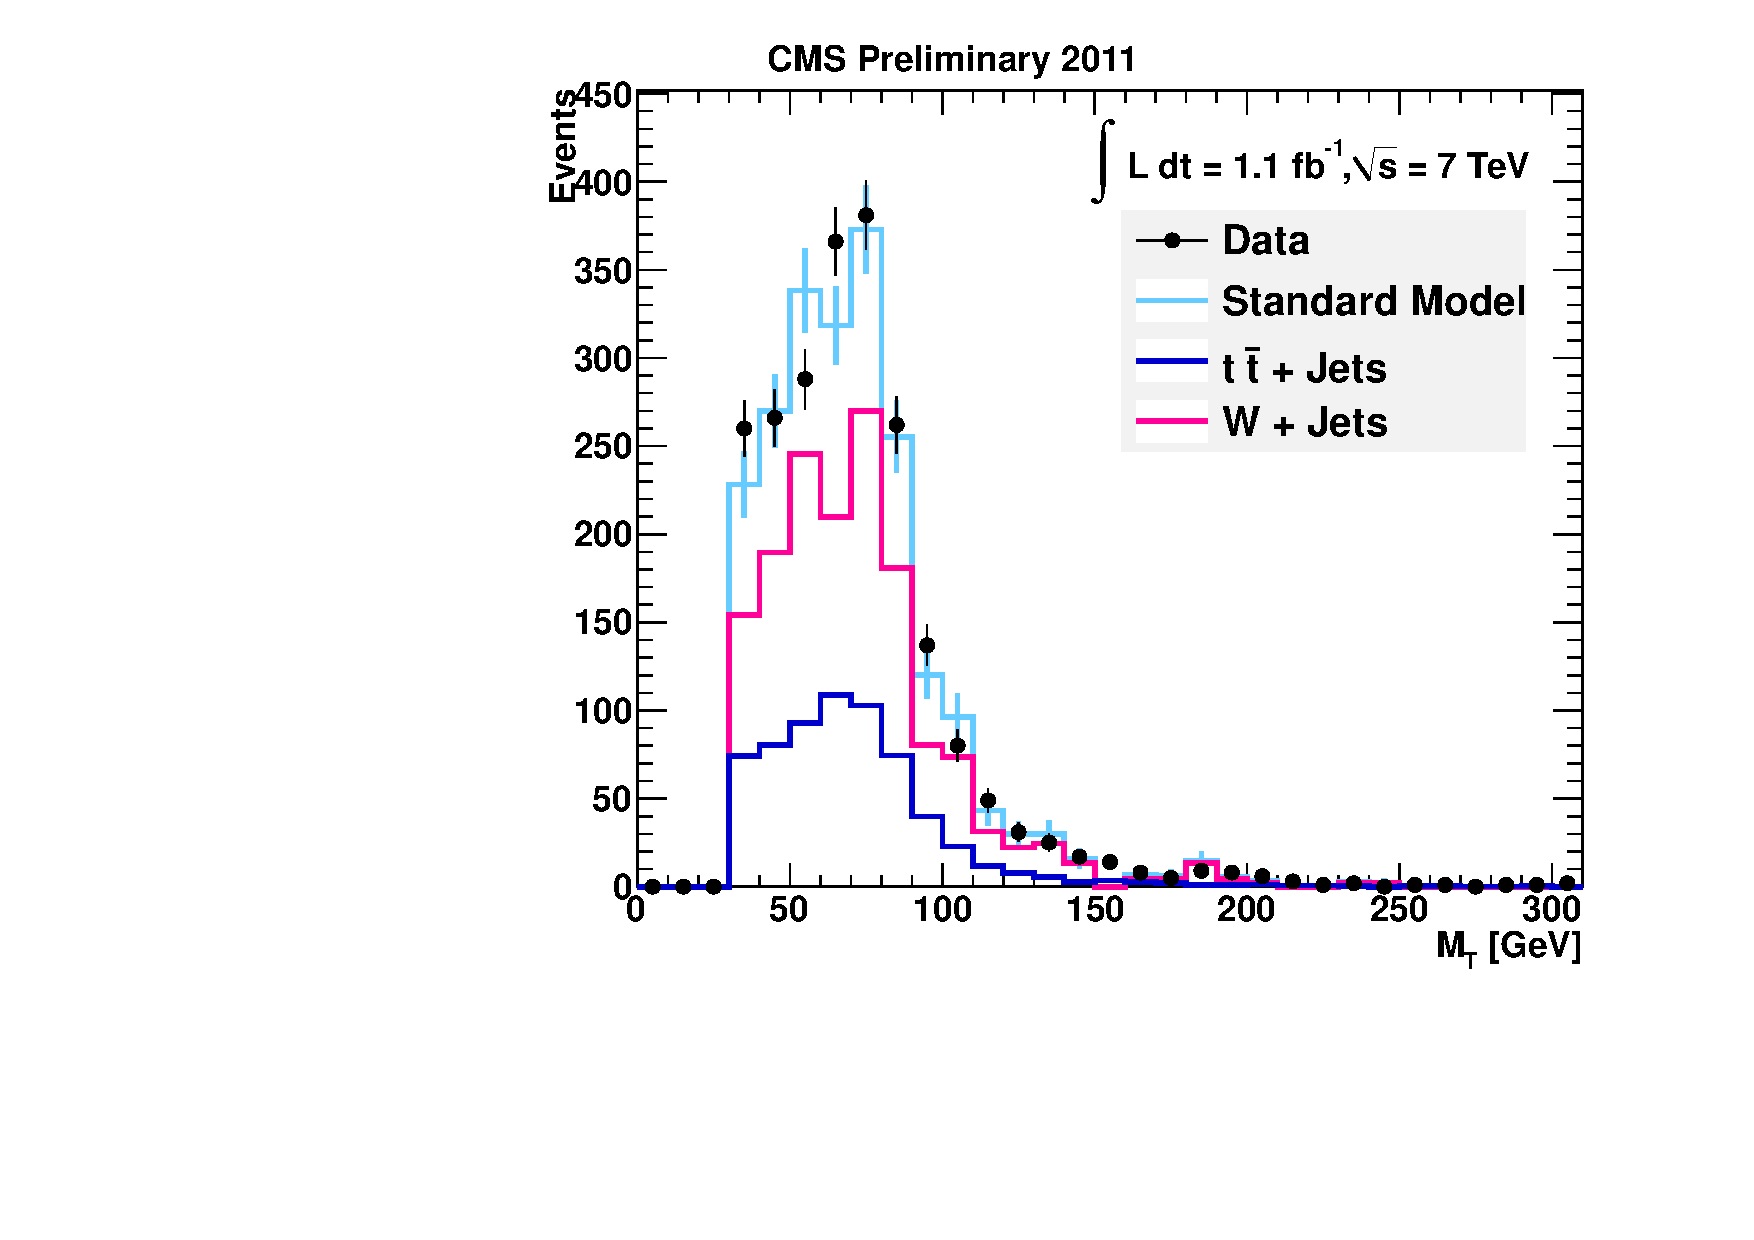
\includegraphics[width=0.45\textwidth, angle=0]{Figures/Analysis/PAS/muon_plots/spring11NoLogYMTMuonControl_beforeaT.pdf}}

\caption{\label{fig:muonplots_beforeat} Data - Monte Carlo comparisons
  for the muon control selection before the $\alpha_{T} > 0.55$ cut is
  applied, shown for (a) $\alpha_{T}$ and (b) $H_{T}$, (c) Muon  Combined Isolation and (d) $M_{T}$.
 A cut of $\mathrm{HT >}$375 GeV has been applied, to select the
 region of fixed jet thresholds.}
\label{fig:kin}
\end{center}
\end{figure}

\begin{figure}[h]
\begin{center}
\subfigure[\label{fig:muon_beforeat_mupt}]{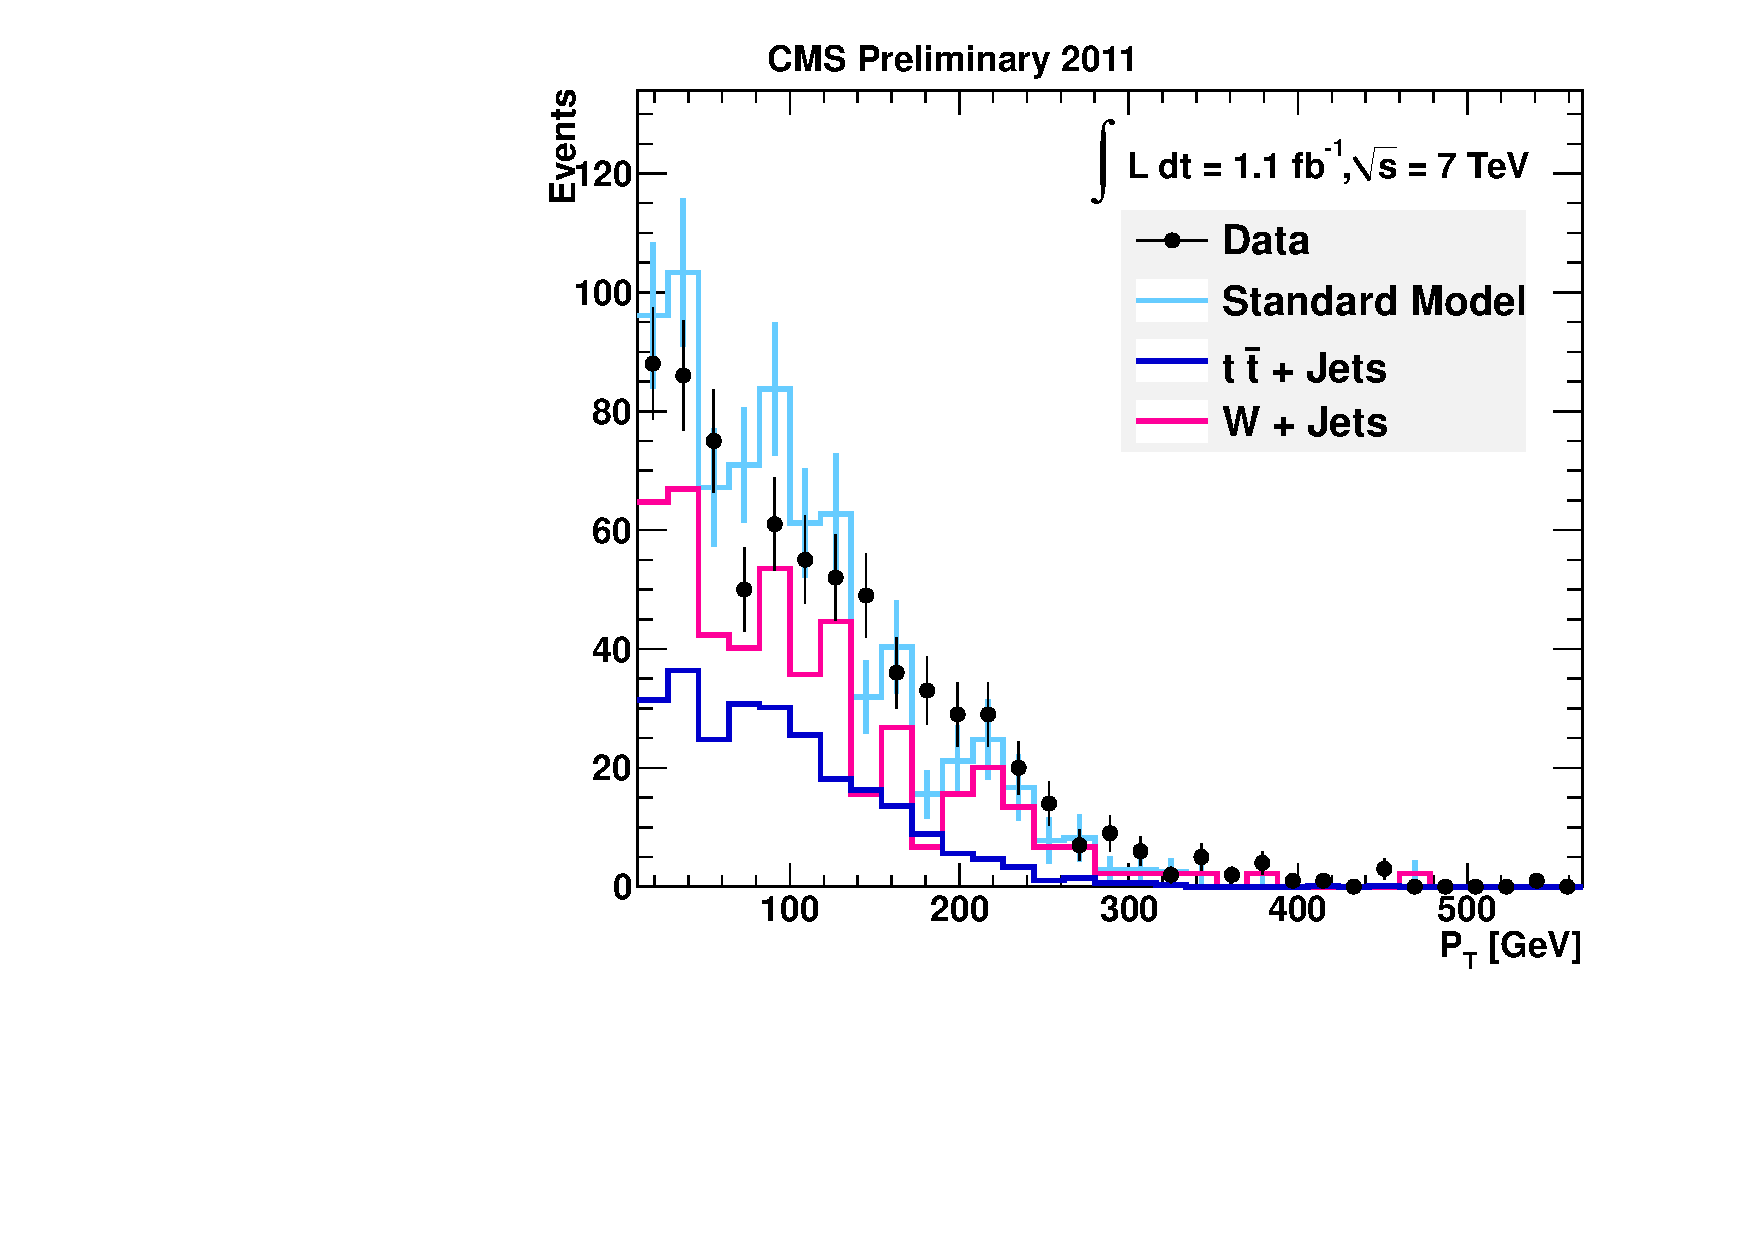
\includegraphics[width=0.45\textwidth, angle=0]{Figures/Analysis/PAS/muon_plots/spring11NoLogYMuPtMuonControl_afteraT.pdf}}
\subfigure[\label{fig:muon_beforeat_njet}]{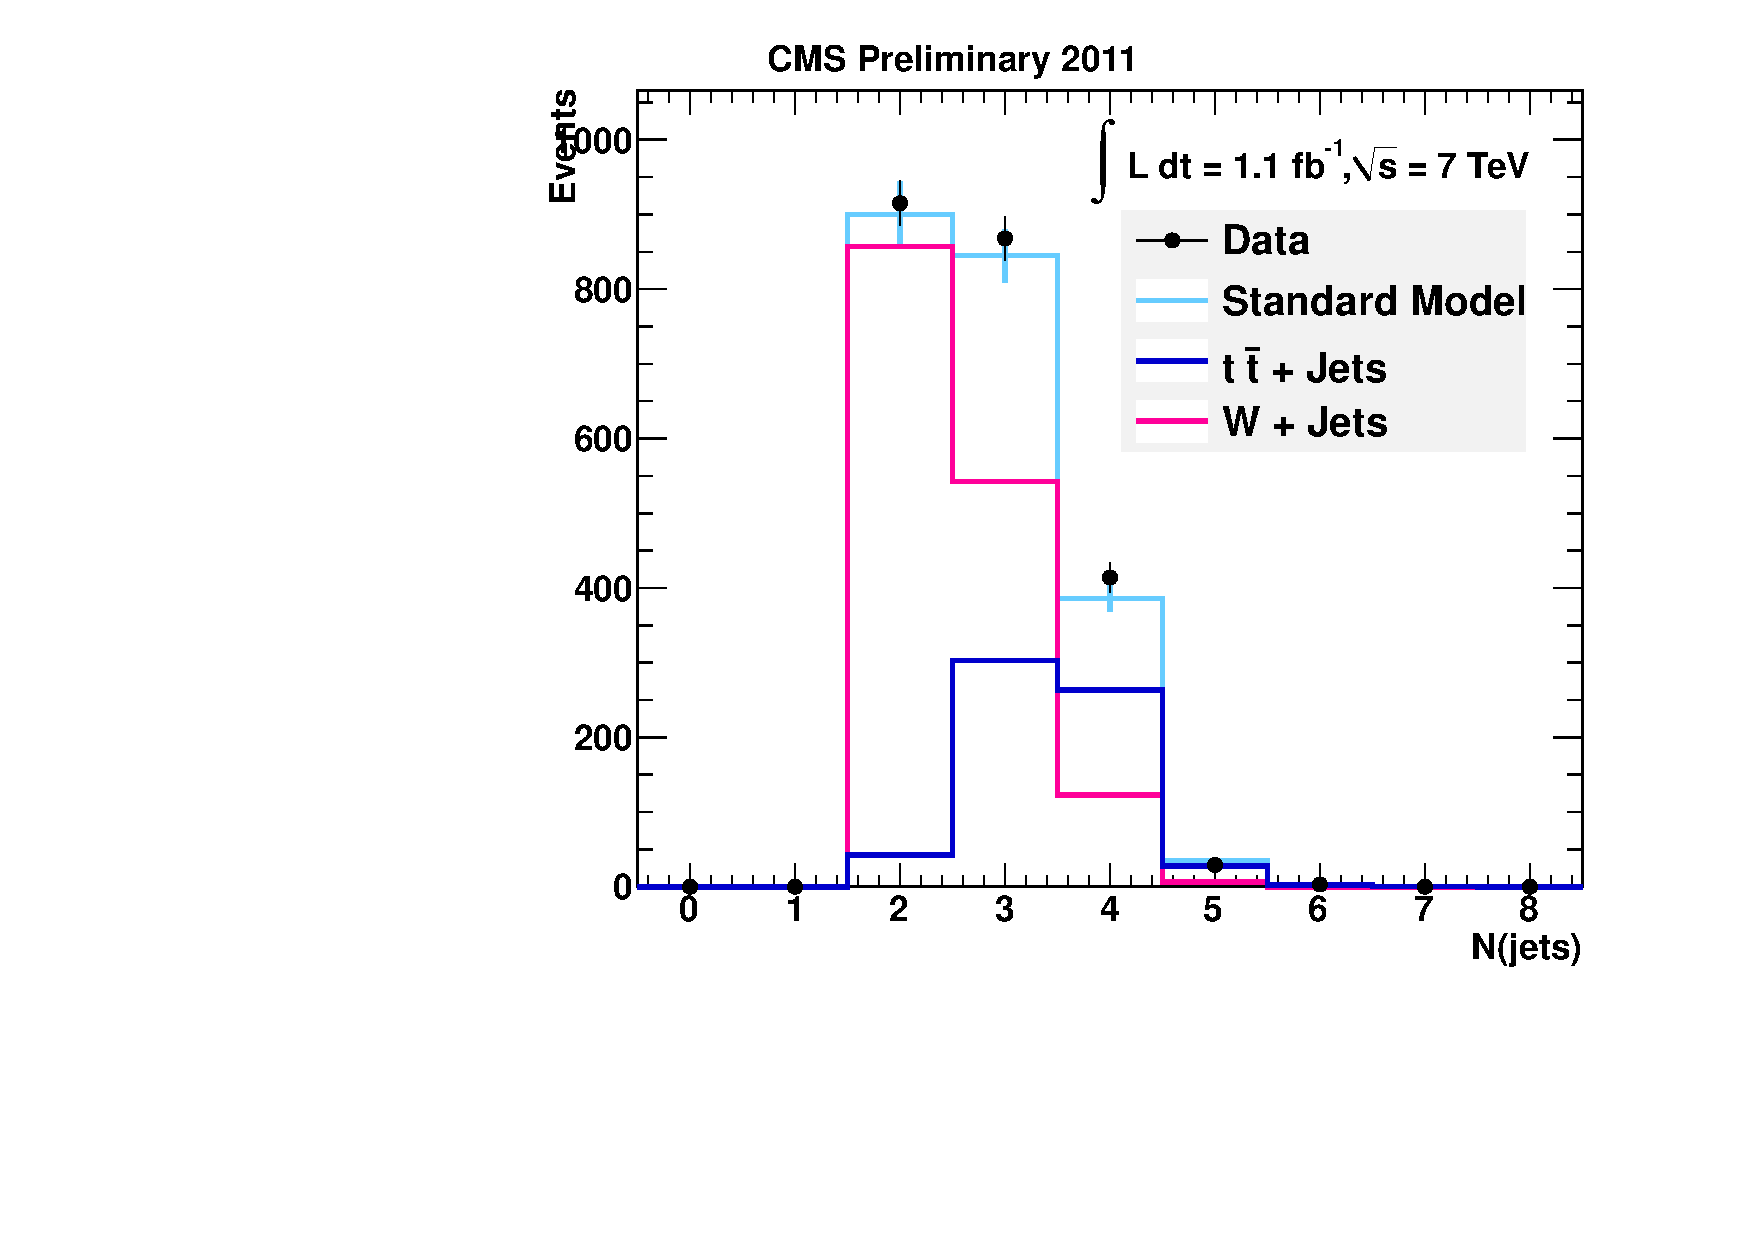
\includegraphics[width=0.45\textwidth, angle=0]{Figures/Analysis/PAS/muon_plots/spring11NoLogYnJetMuonControl_beforeaT.pdf}}
\newline

\subfigure[\label{fig:muon_afterat_at}]{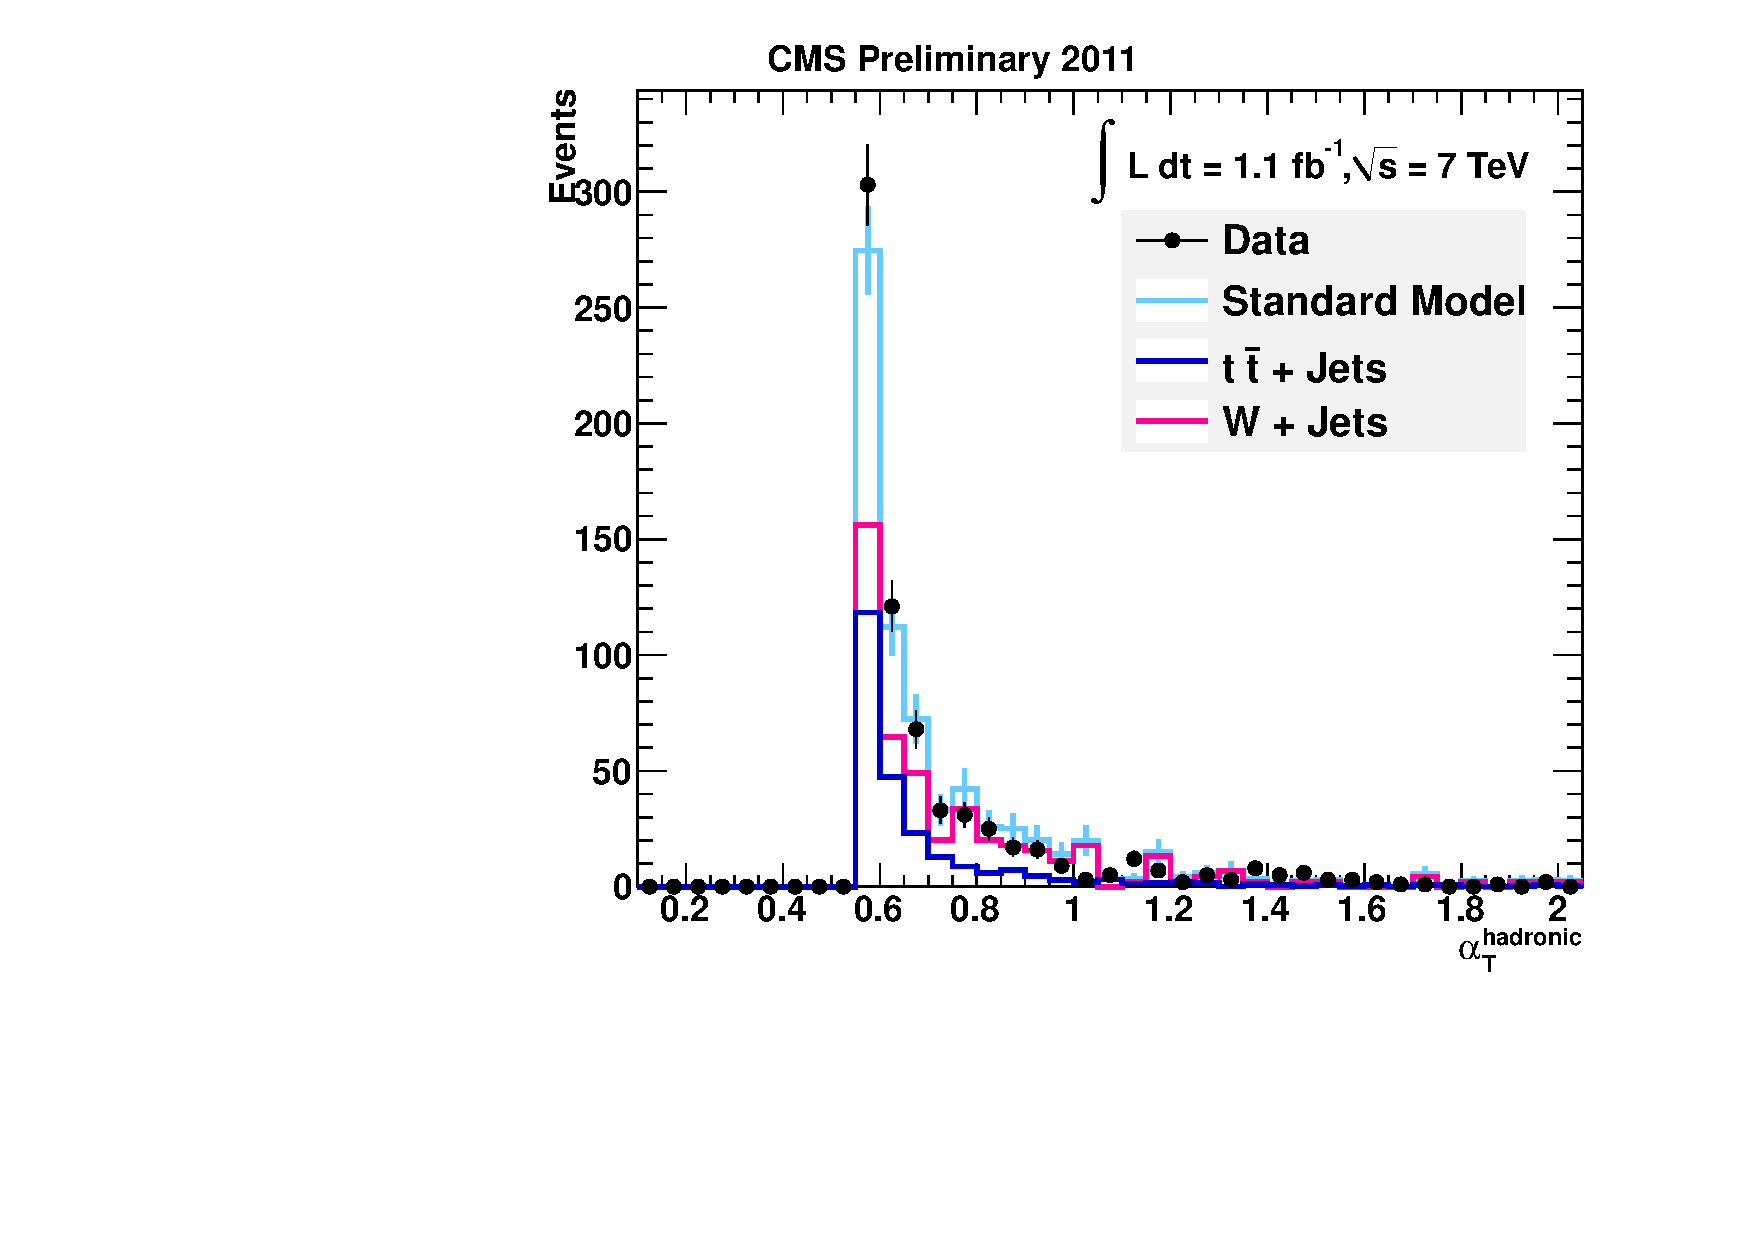
\includegraphics[width=0.45\textwidth, angle=0]{Figures/Analysis/PAS/muon_plots/spring11NoLogYaT_HMuonControl_afteraT.pdf}}
\subfigure[\label{fig:muon_afterat_ht}]{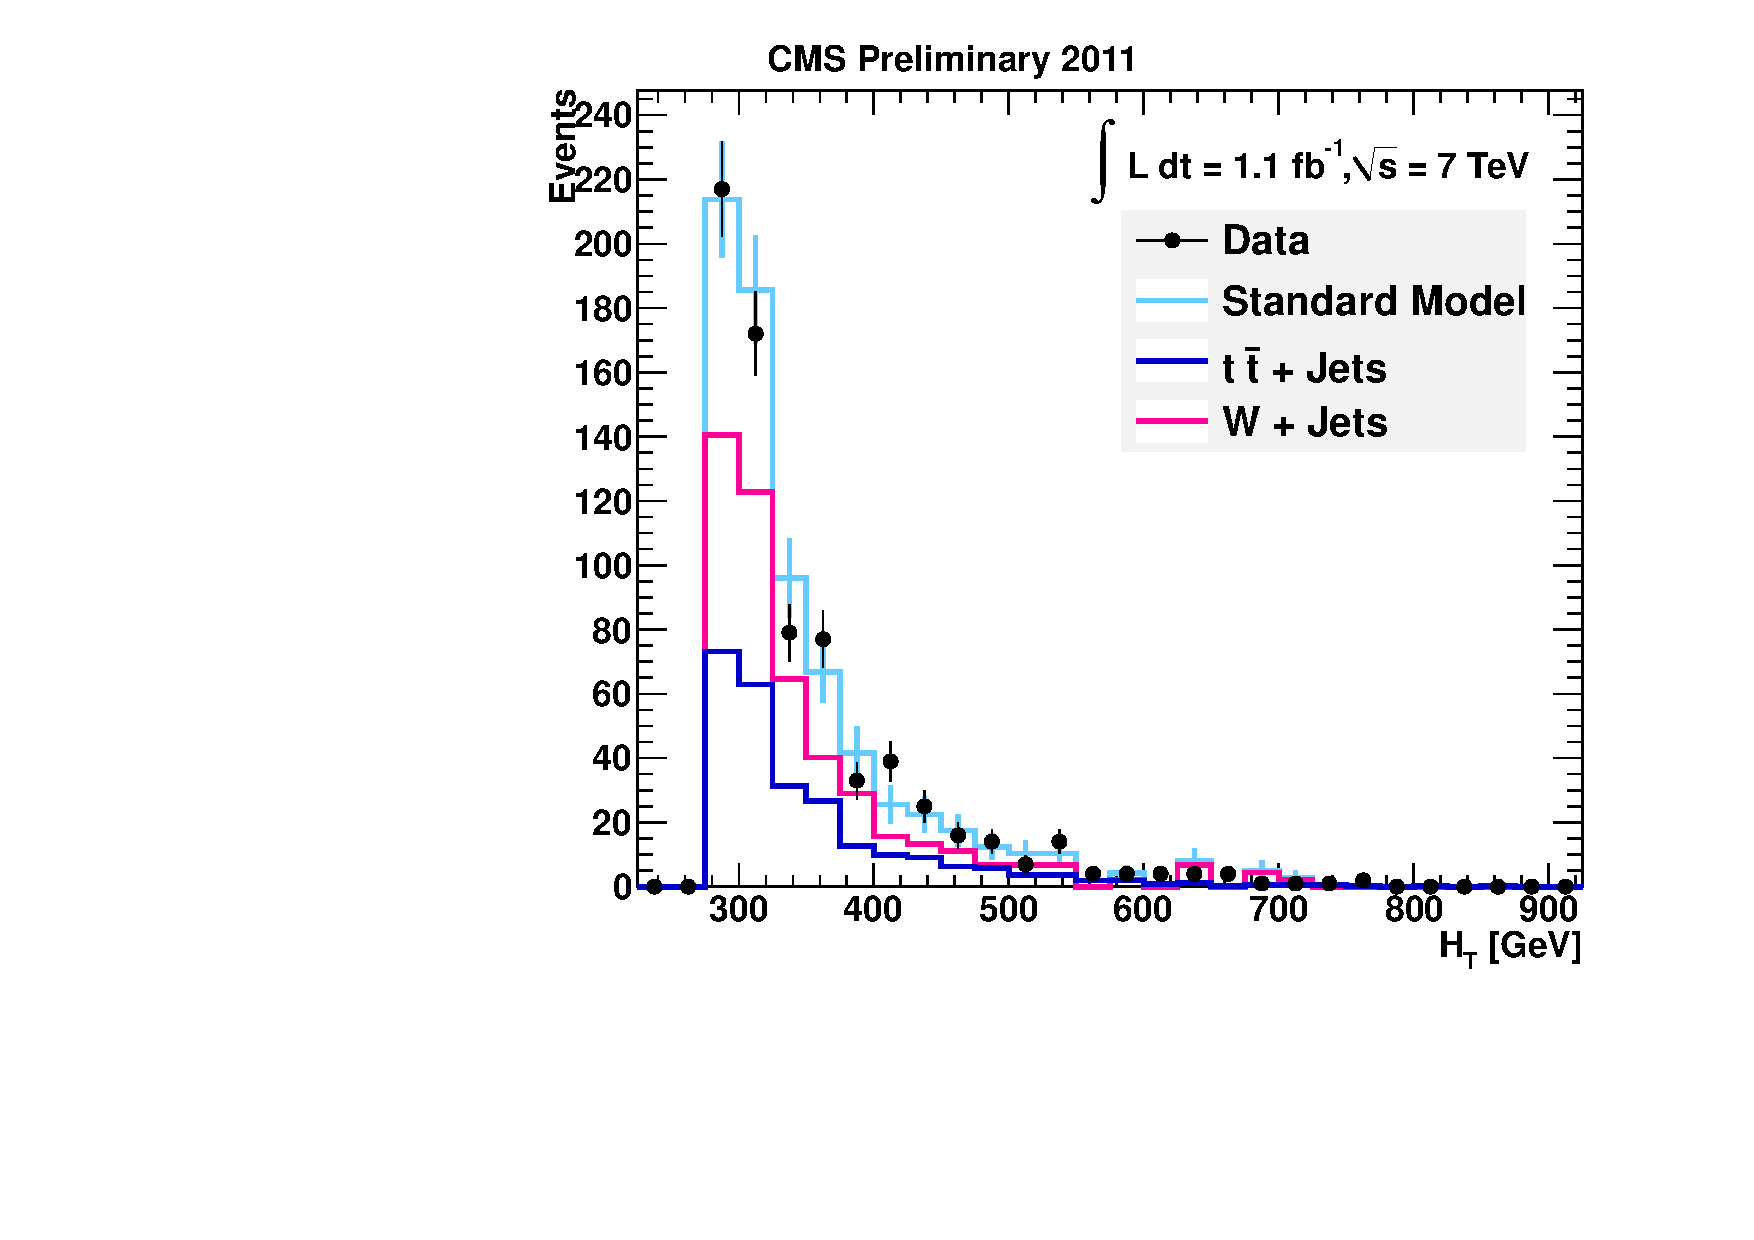
\includegraphics[width=0.45\textwidth, angle=0]{Figures/Analysis/PAS/muon_plots/spring11NoLogYHTMuonControl_afteraT.pdf}}
\newline
\subfigure[\label{fig:muon_afterat_MuIso}]{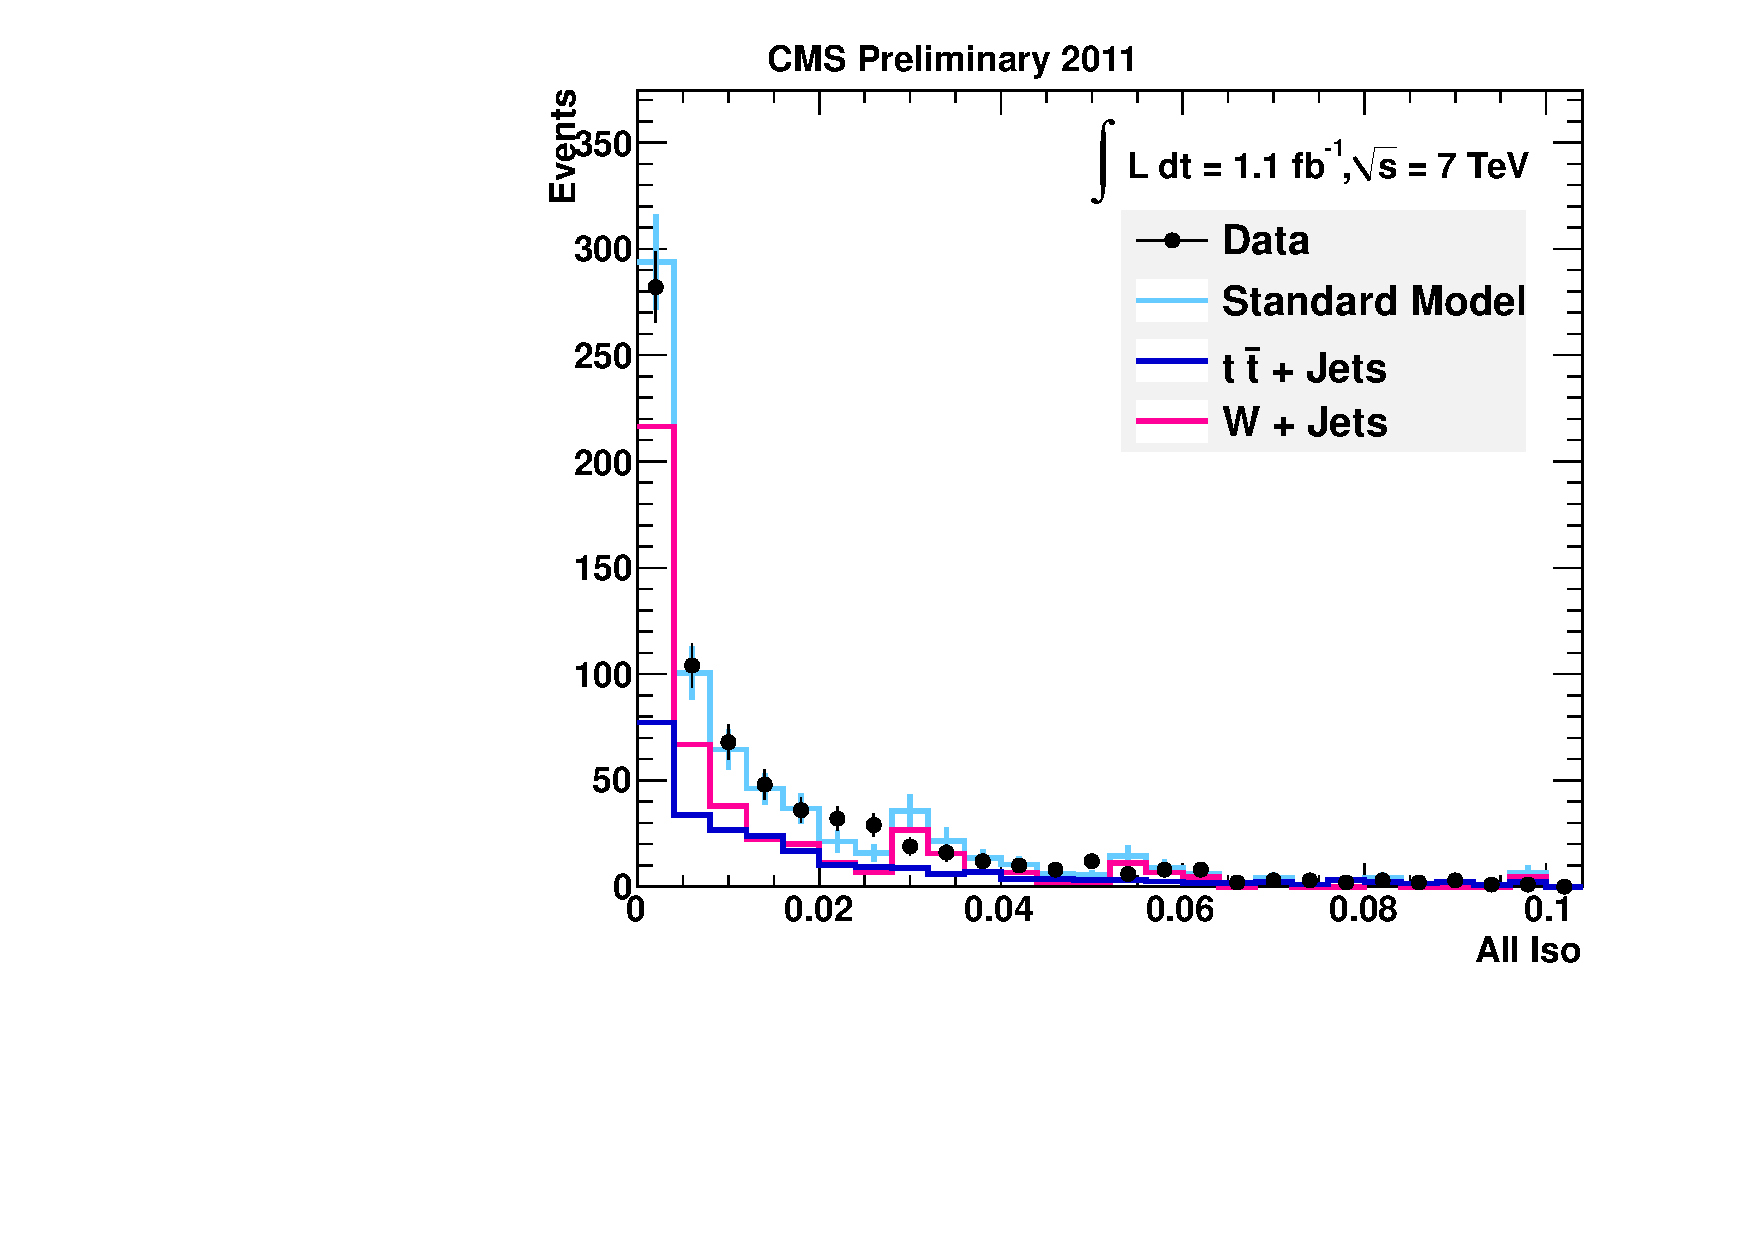
\includegraphics[width=0.45\textwidth, angle=0]{Figures/Analysis/PAS/muon_plots/spring11NoLogYMuCsoMuonControl_afteraT.pdf}}
\subfigure[\label{fig:muon_afterat_mt}]{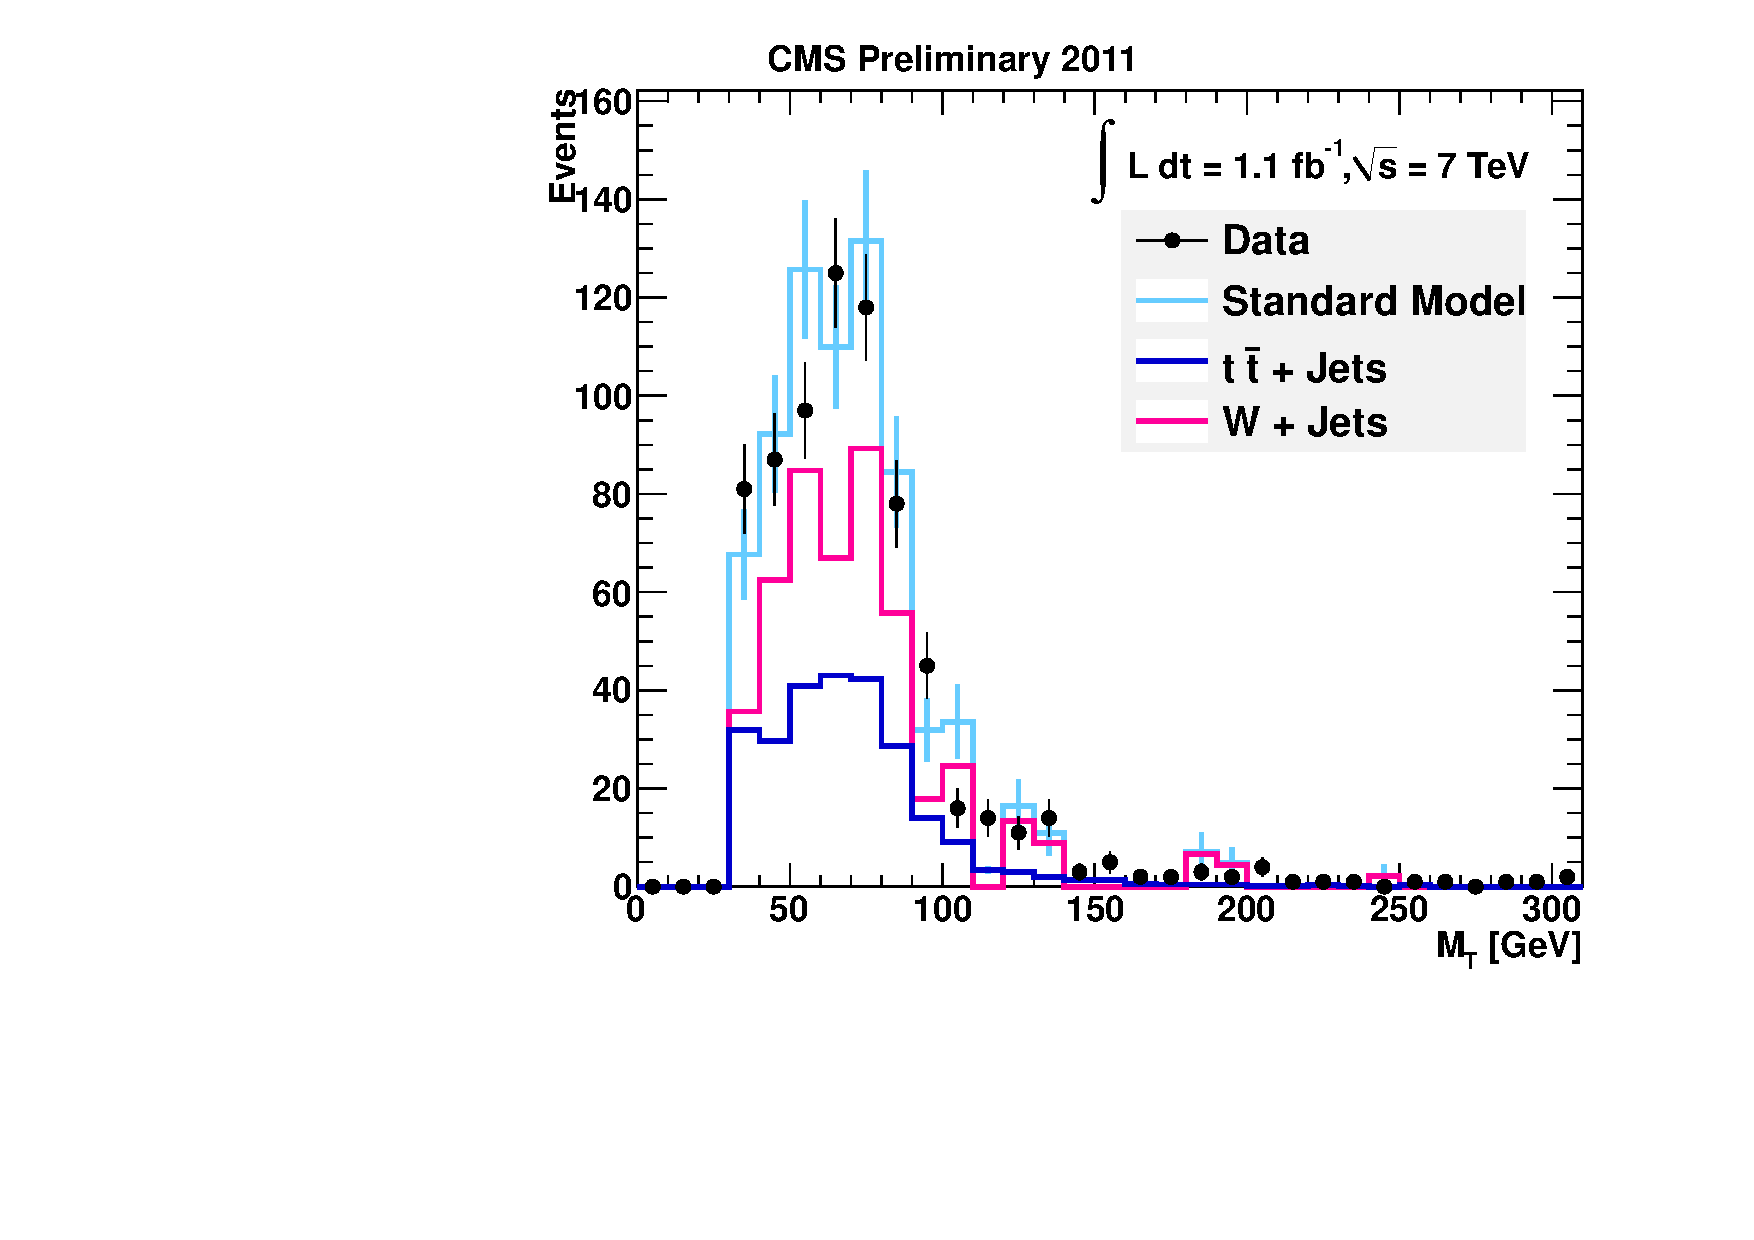
\includegraphics[width=0.45\textwidth, angle=0]{Figures/Analysis/PAS/muon_plots/spring11NoLogYMTMuonControl_afteraT.pdf}}

\caption{\label{fig:muonplots_afterat} Data - Monte Carlo comparisons
  for the muon control selection after the $\alpha_{T} > 0.55$ cut is
  applied, shown for (a) \scalht and (b) $M_T$, (c) Muon  Combined Isolation and (d) $M_{T}$.
 A cut of $\mathrm{HT >}$375 GeV has been applied, to select the
 region of fixed jet thresholds.}
\label{fig:kin}
\end{center}
\end{figure}

\subsubsection{Types of decay contributing to Muon Control Sample}

\begin{figure}[h]
\begin{center}
\subfigure[\label{fig:muon_types_275TT}]{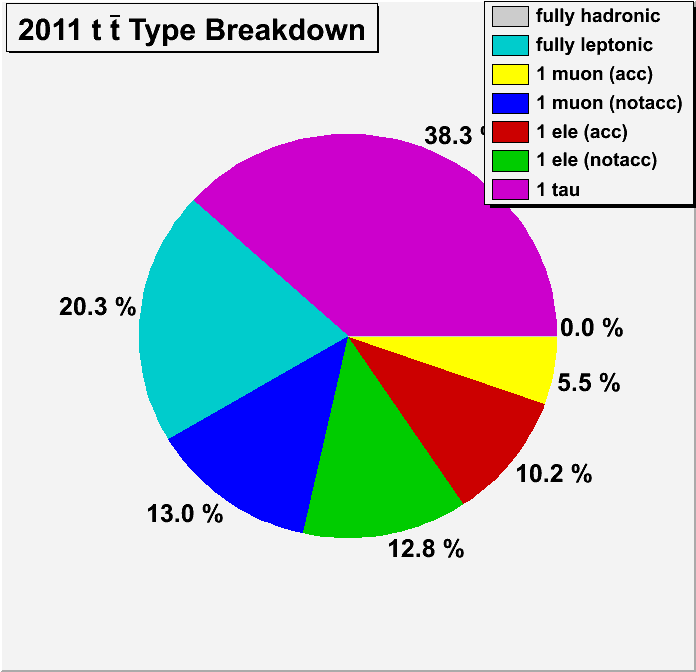
\includegraphics[width=0.40\textwidth, angle=0]{Figures/Analysis/Types/2011_275_TT_Pie}}
\subfigure[\label{fig:muon_types_275W}] {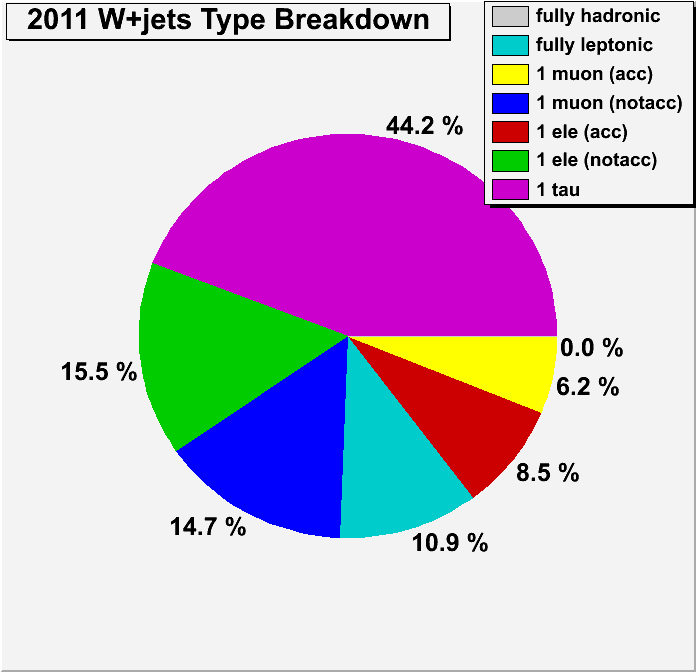
\includegraphics[width=0.40\textwidth, angle=0]{Figures/Analysis/Types/2011_275_W_Pie}}
\newline
\subfigure[\label{fig:muon_types_325TT}]{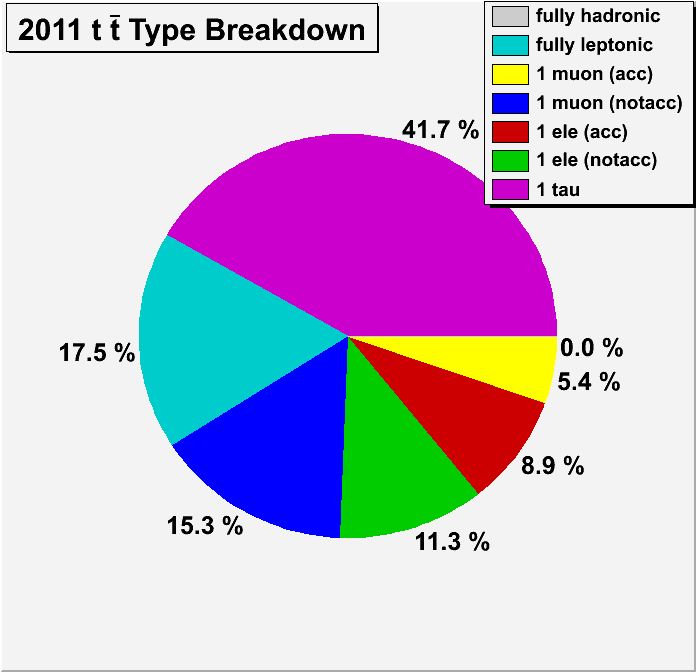
\includegraphics[width=0.40\textwidth, angle=0]{Figures/Analysis/Types/2011_325_TT_Pie}}
\subfigure[\label{fig:muon_types_325W}] {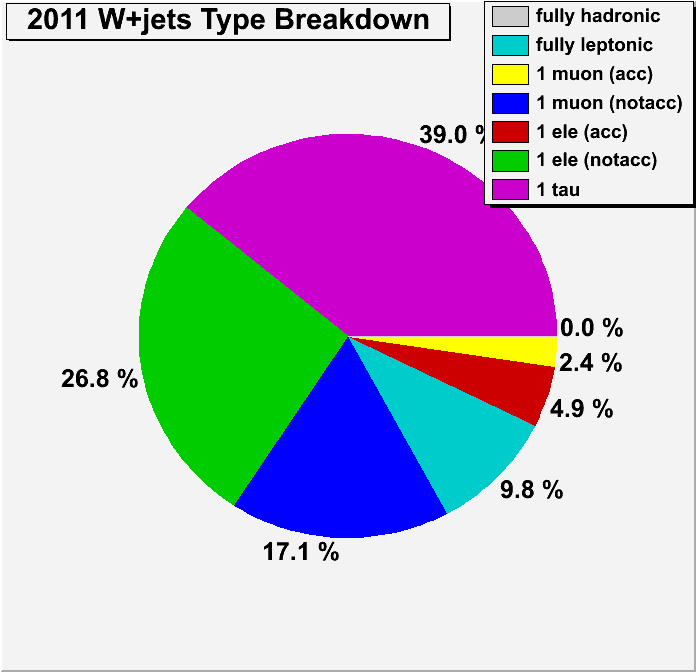
\includegraphics[width=0.40\textwidth, angle=0]{Figures/Analysis/Types/2011_325_W_Pie}}
\newline
\subfigure[\label{fig:muon_types_allTT}]{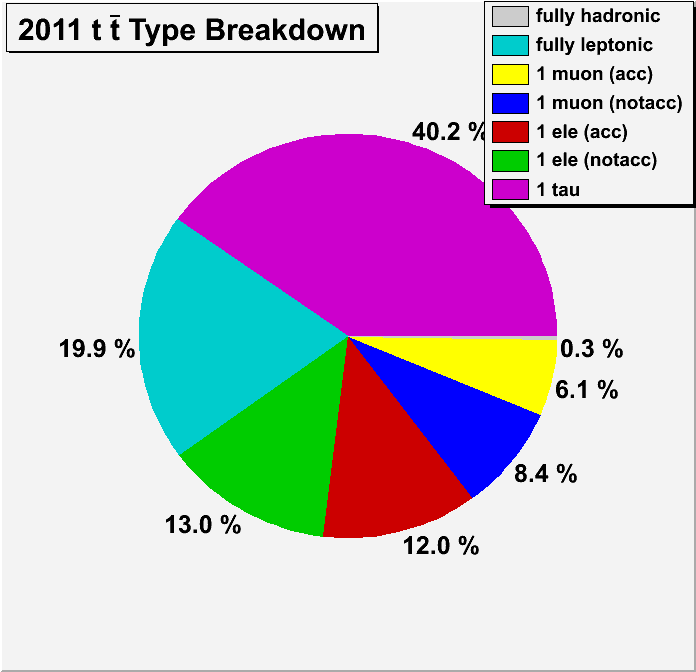
\includegraphics[width=0.40\textwidth, angle=0]{Figures/Analysis/Types/2011_unsca375_TT_Pie}}
\subfigure[\label{fig:muon_types_allW}] {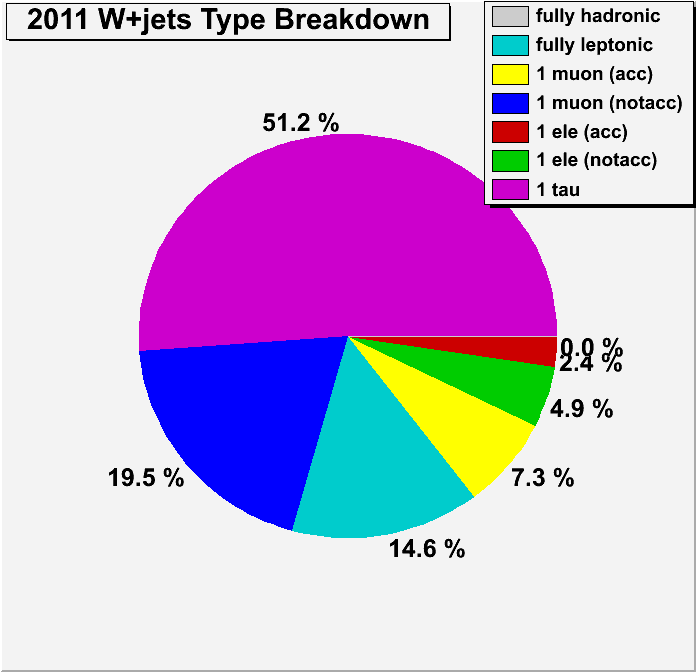
\includegraphics[width=0.40\textwidth, angle=0]{Figures/Analysis/Types/2011_unsca375_W_Pie}}

\caption{\label{fig:muon_types} Type breakdown of decays resulting in an event selected by the Muon Control selection, shown using Monte-Carlo truth information separately for \ttj (left) and \wj (right) events. The breakdown is made separately for each jet-scale case: 275 \less \HT \less 325 GeV (top), 325 \less \HT \less 375 GeV (middle), and \HT \more 375 GeV (bottom). }
\end{center}
\end{figure}

\subsection{Estimation Z  $\nu \bar{\nu}$ + jets background using photon + jets events}

\begin{figure}[h]
\begin{center}
\subfigure[\label{fig:photon_alphaT}]{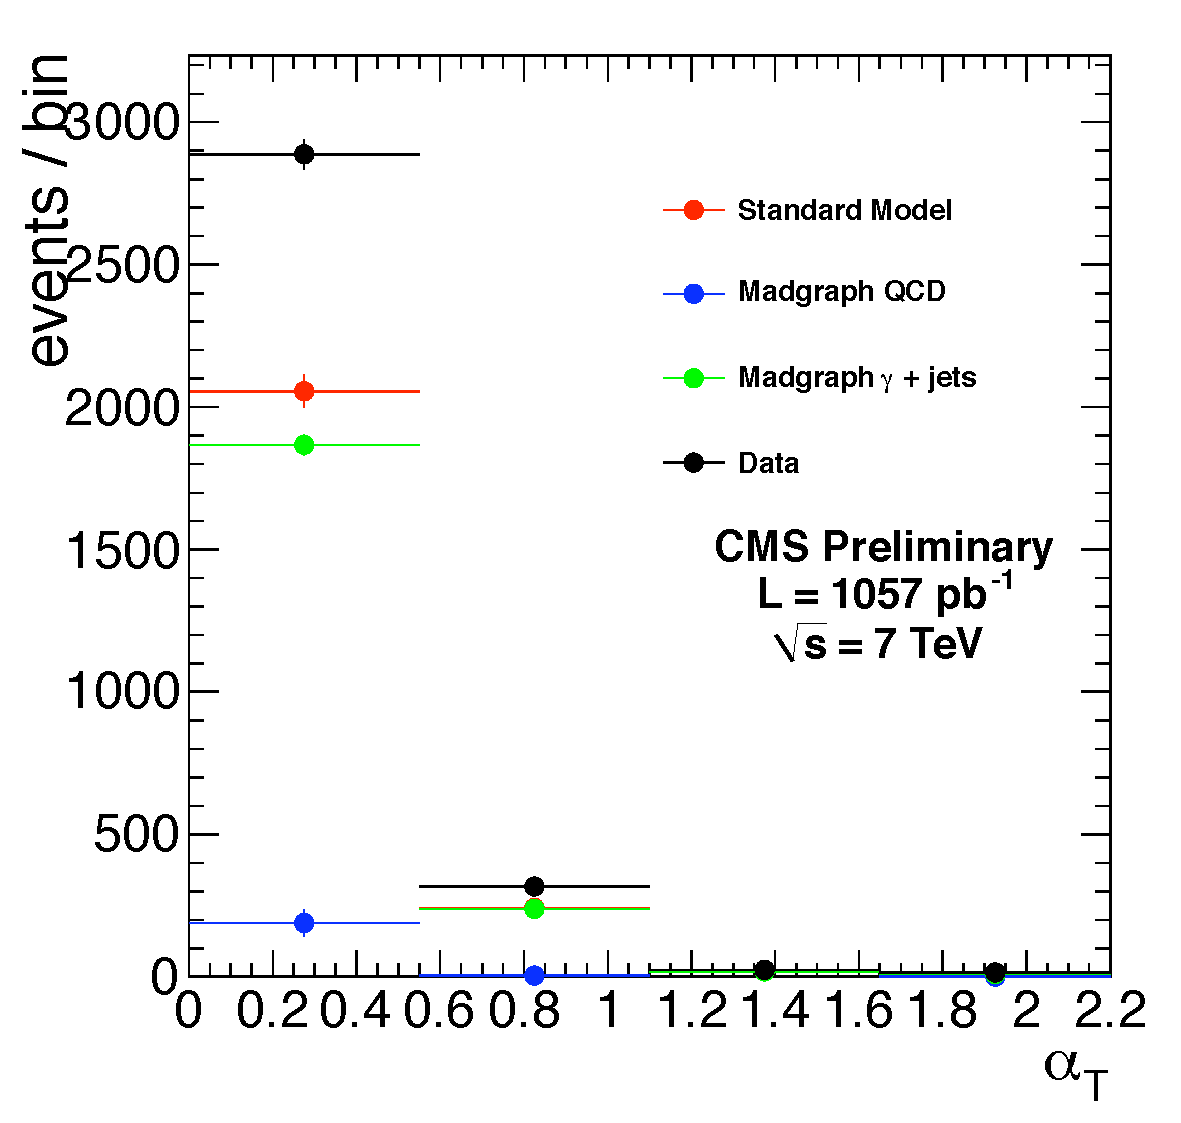
\includegraphics[width=0.45\textwidth, angle=0]{Figures/Analysis/PAS/photon_plots/375___xcak5JetAlphaTFewBinsPat.pdf}}
\subfigure[\label{fig:photon_nJets}] {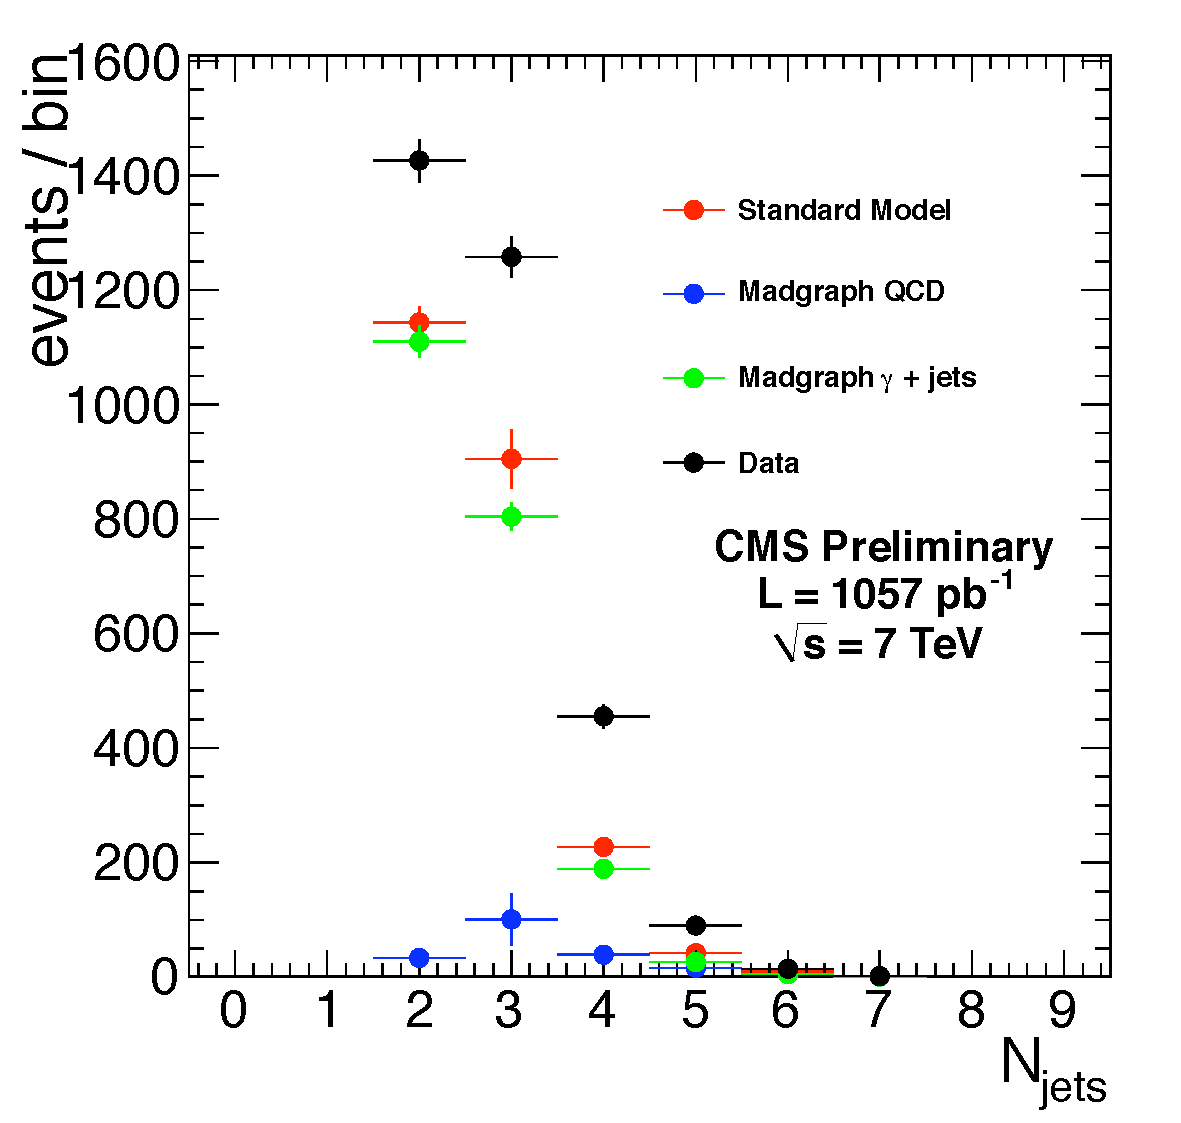
\includegraphics[width=0.45\textwidth, angle=0]{Figures/Analysis/PAS/photon_plots/375___xcak5JetIndicesPat.pdf}}
\caption{\label{fig:photon_plots} Data-MC comparisons for the photon control sample.  $\scalht > 375$~GeV and $\mht/\scalht>0.4$ are required.   Left: the distribution of $\alpha_{T}$.  Right: the distribution of the number of jets.}
\end{center}
\end{figure}

\section{Systematic Uncertainties}
\section{Simultaneous Fit}


 \begin{figure}[h]
   \begin{center}
     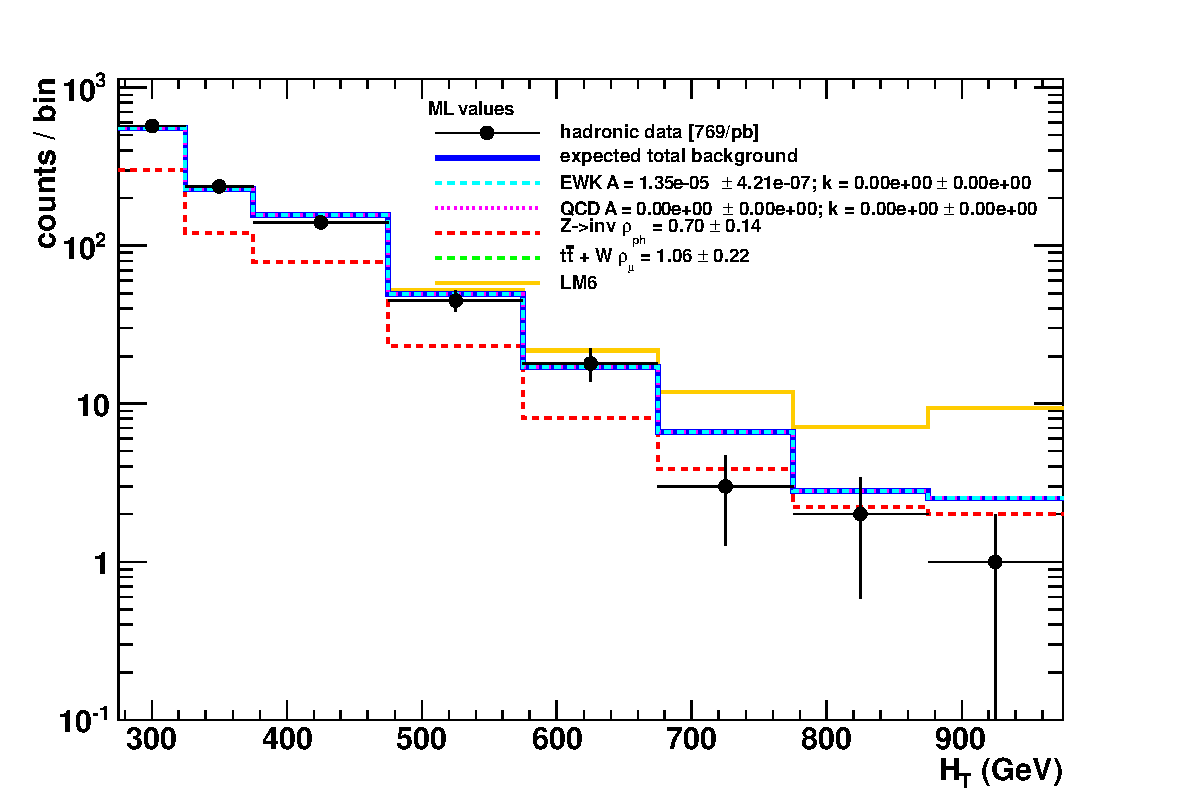
\includegraphics[width = 0.48\textwidth]{Figures/Analysis/PAS/stats_plots/RQcdZero/hadronic_signal_fit_logy.pdf}
     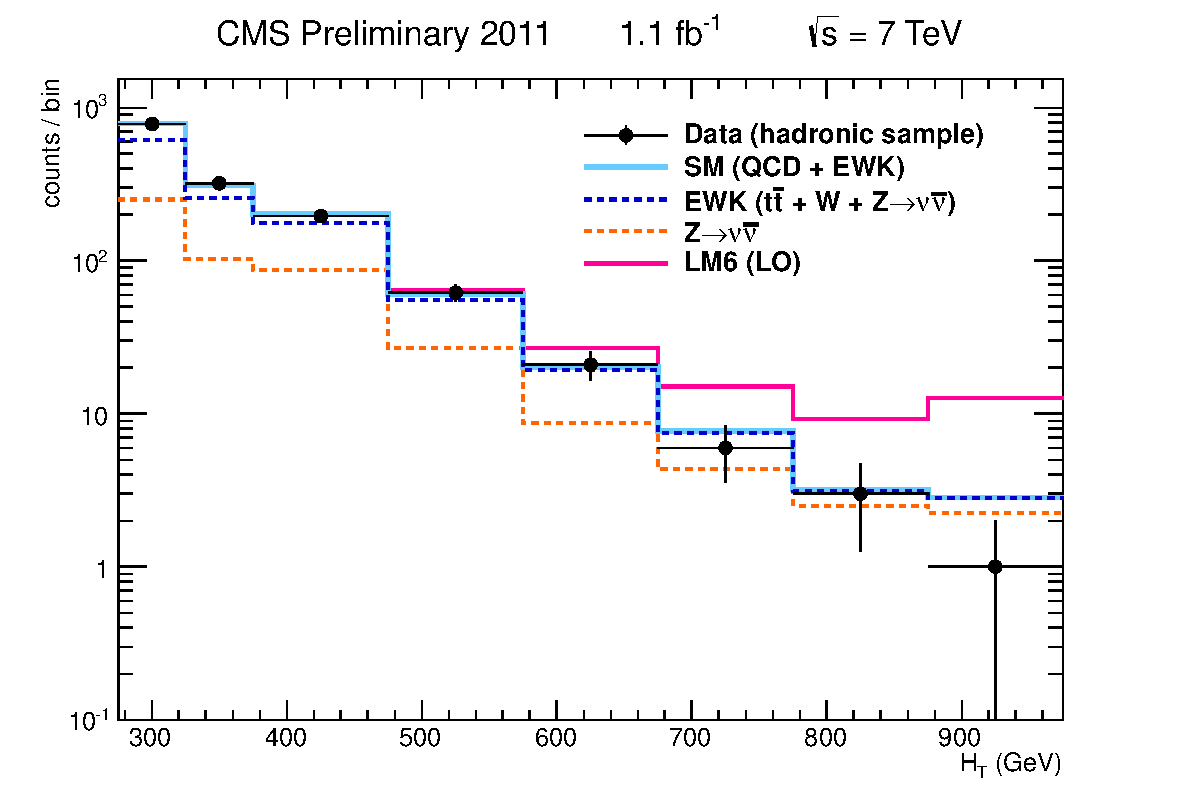
\includegraphics[width = 0.48\textwidth]{Figures/Analysis/PAS/stats_plots/RQcdFallingExp/hadronic_signal_fit_logy.pdf}
     \caption{\label{fig:hadronic} \scalht distribution for events in the hadronic signal sample for scenario a) (left) and scenario b) (right). Shown are the events observed in data (black points), the outcome of the fit (blue line) and a breakdown of the individual background contributions as predicted by the control samples. A possible signal contribution from benchmark point LM6 is indicated as well (yellow line).}
   \end{center}
 \end{figure}

 \begin{figure}[h]
   \begin{center}
     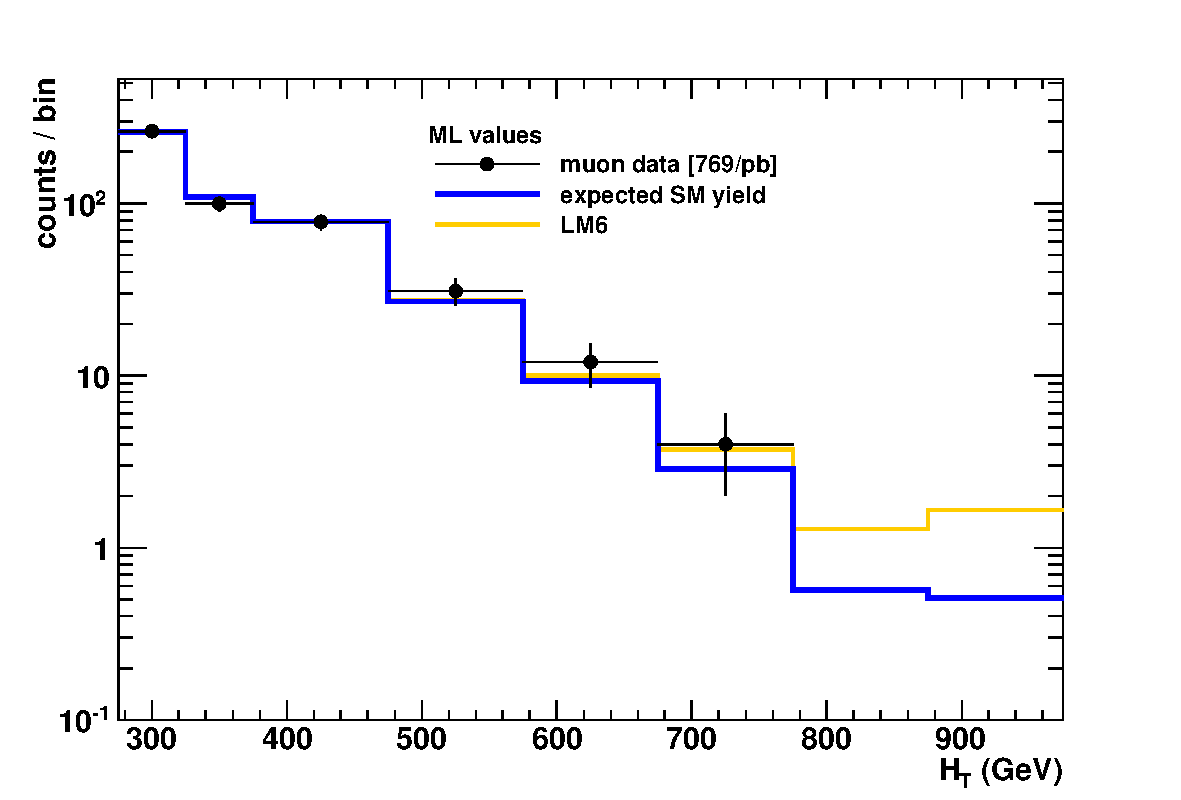
\includegraphics[width = 0.48\textwidth]{Figures/Analysis/PAS/stats_plots/RQcdZero/muon_control_fit_logy.pdf}
     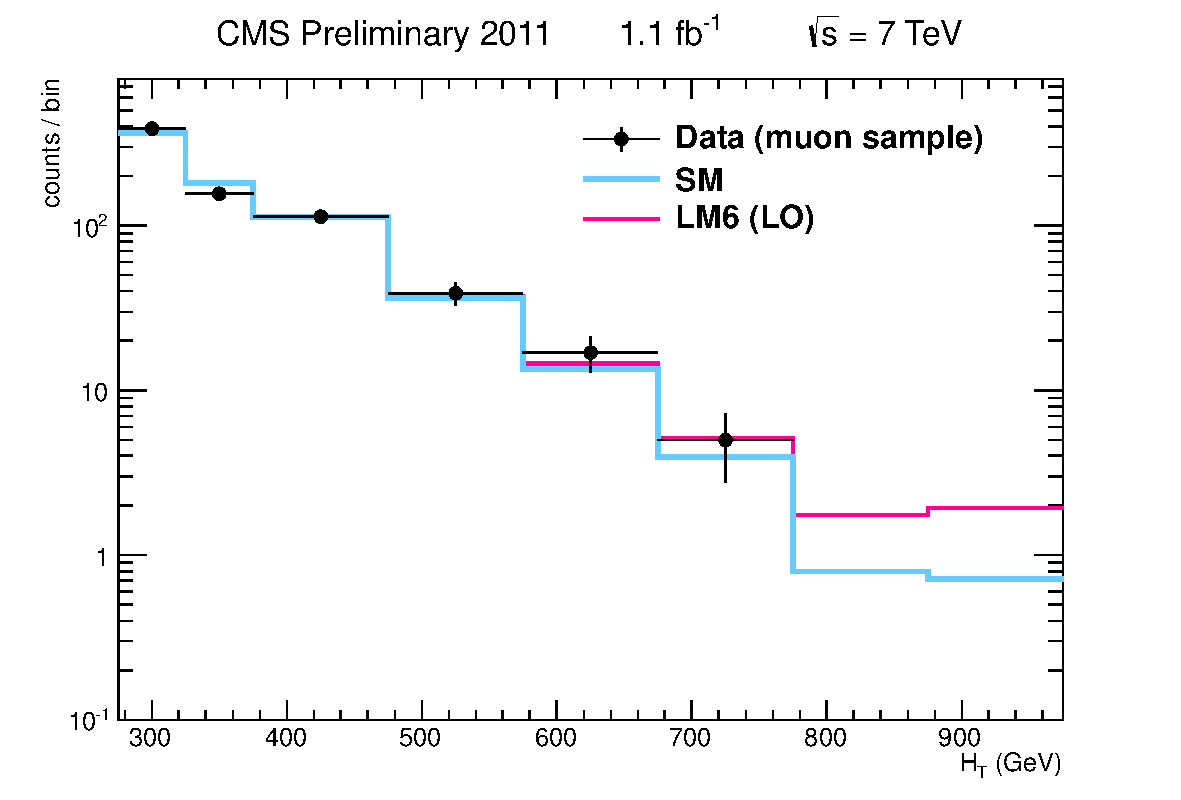
\includegraphics[width = 0.48\textwidth]{Figures/Analysis/PAS/stats_plots/RQcdFallingExp/muon_control_fit_logy.pdf}
     \caption{\label{fig:muon}  \scalht distribution for events selected in the muon control sample for scenario a) (left) and scenario b) (right).
  Shown are the events observed in data (black points), the outcome of the fit (blue line) and the MC expectation (dashed line). A possible signal
 contribution from benchmark point LM6 is indicated as well (yellow line).}
   \end{center}
 \end{figure}

 \begin{figure}[h]
   \begin{center}
     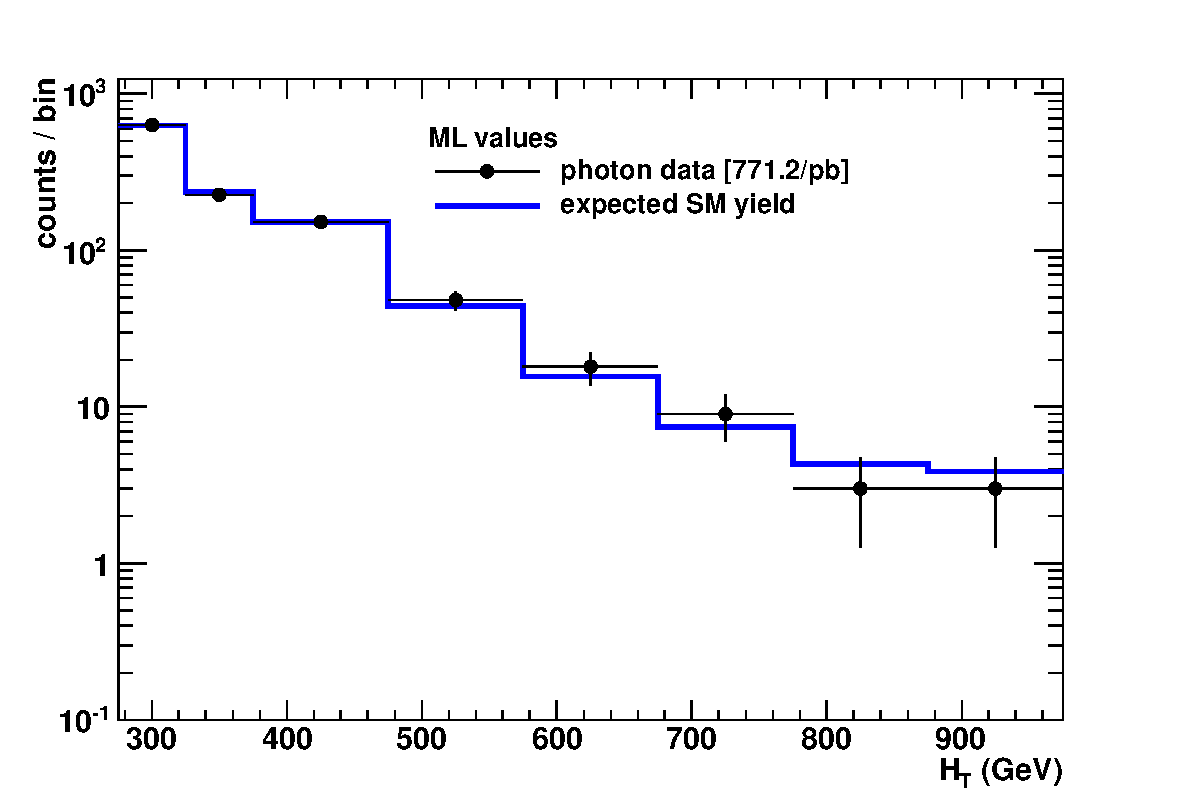
\includegraphics[width = 0.48\textwidth]{Figures/Analysis/PAS/stats_plots/RQcdZero/photon_control_fit_logy.pdf}
     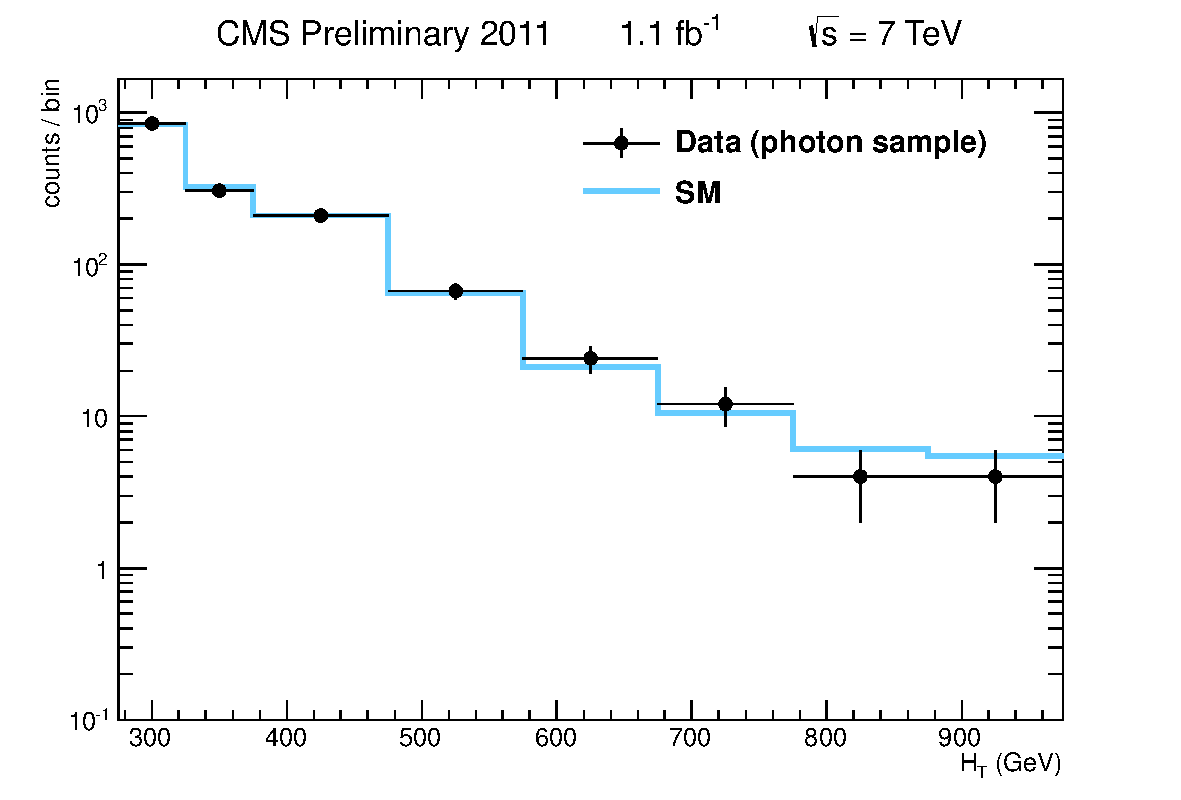
\includegraphics[width = 0.48\textwidth]{Figures/Analysis/PAS/stats_plots/RQcdFallingExp/photon_control_fit_logy.pdf}
     \caption{\label{fig:photon} \scalht distribution for events selected in the photon control sample for scenario a) (left) and scenario b) (right). Shown are the events observed in data (black points), the outcome of the fit (blue line) and the MC expectation (dashed line).}
   \end{center}
 \end{figure}

 \begin{figure}[h]
   \begin{center}
     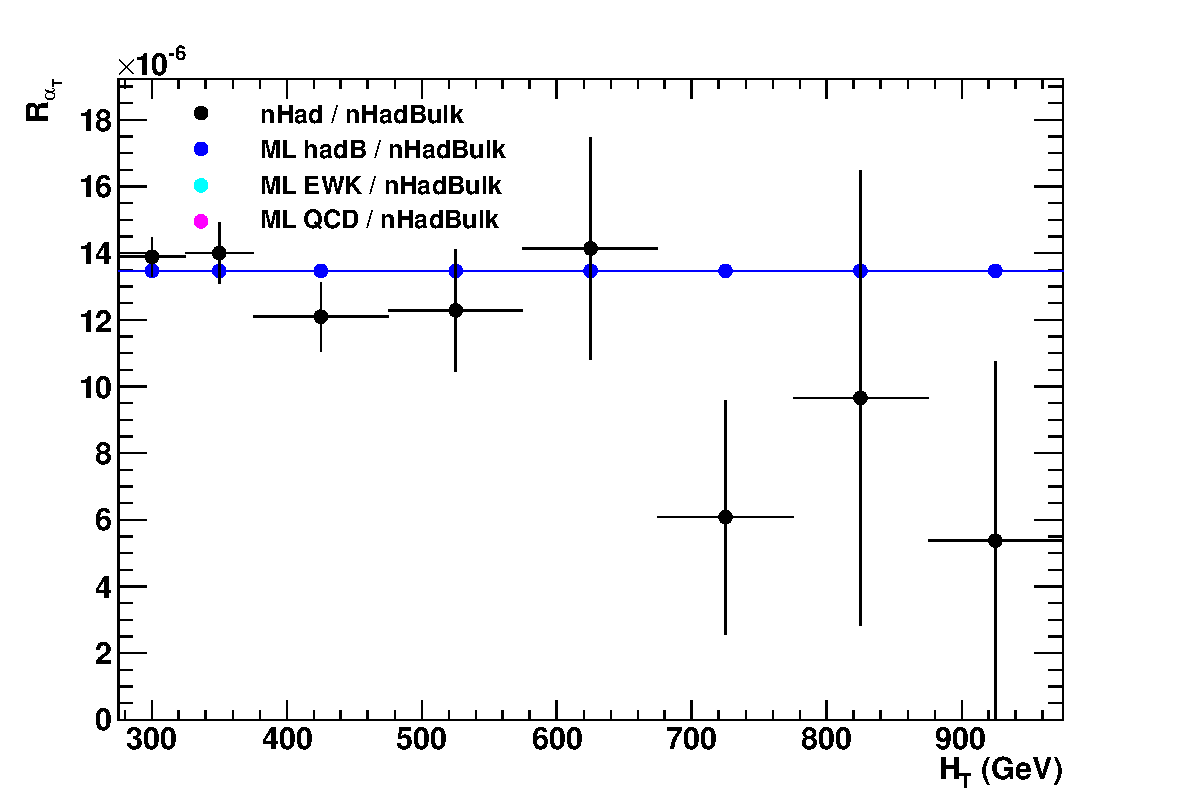
\includegraphics[width = 0.48\textwidth]{Figures/Analysis/PAS/stats_plots/RQcdZero/hadronic_signal_alphaT_ratio.pdf}
     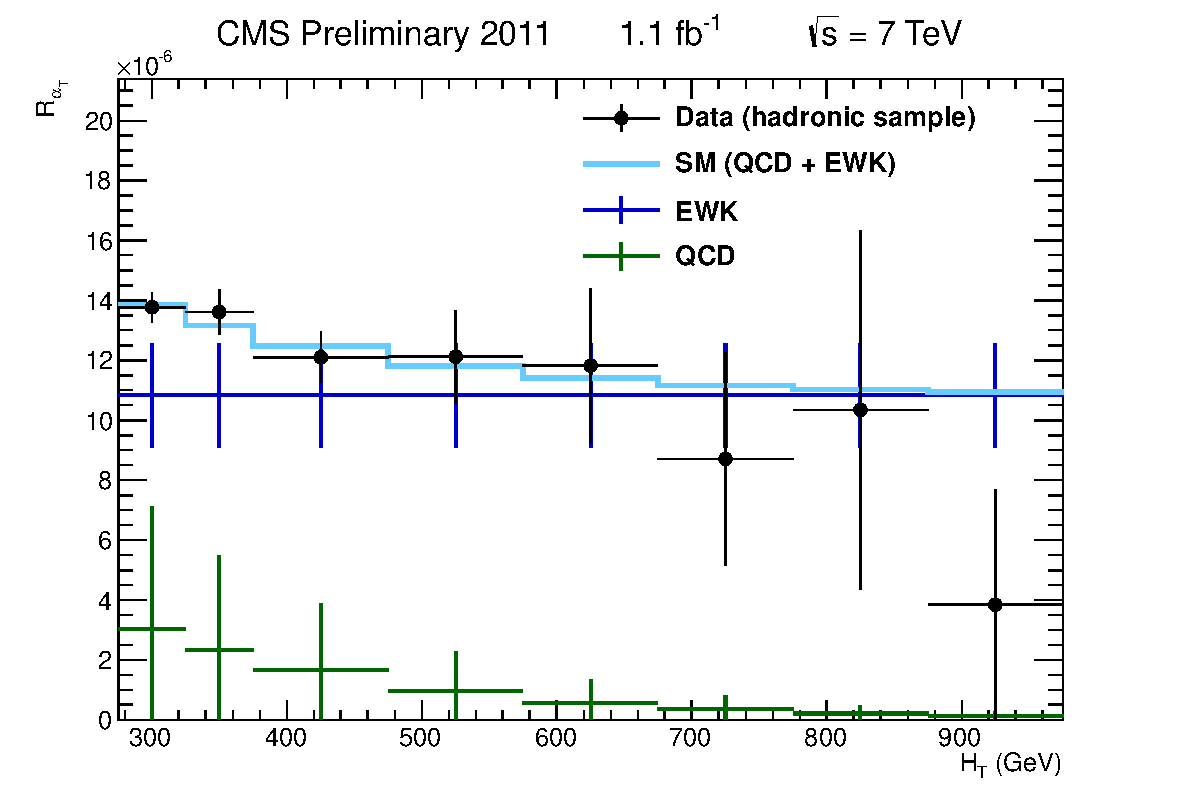
\includegraphics[width = 0.48\textwidth]{Figures/Analysis/PAS/stats_plots/RQcdFallingExp/hadronic_signal_alphaT_ratio.pdf}
     \caption{\label{fig:rat} \RaT as a function of \scalht as observed in data (black points) and the results of the fit assuming different scenarios: a) (left) and b) (right) .}
   \end{center}
 \end{figure}

\section{Limits}

\begin{figure}[h]
  \begin{center}
    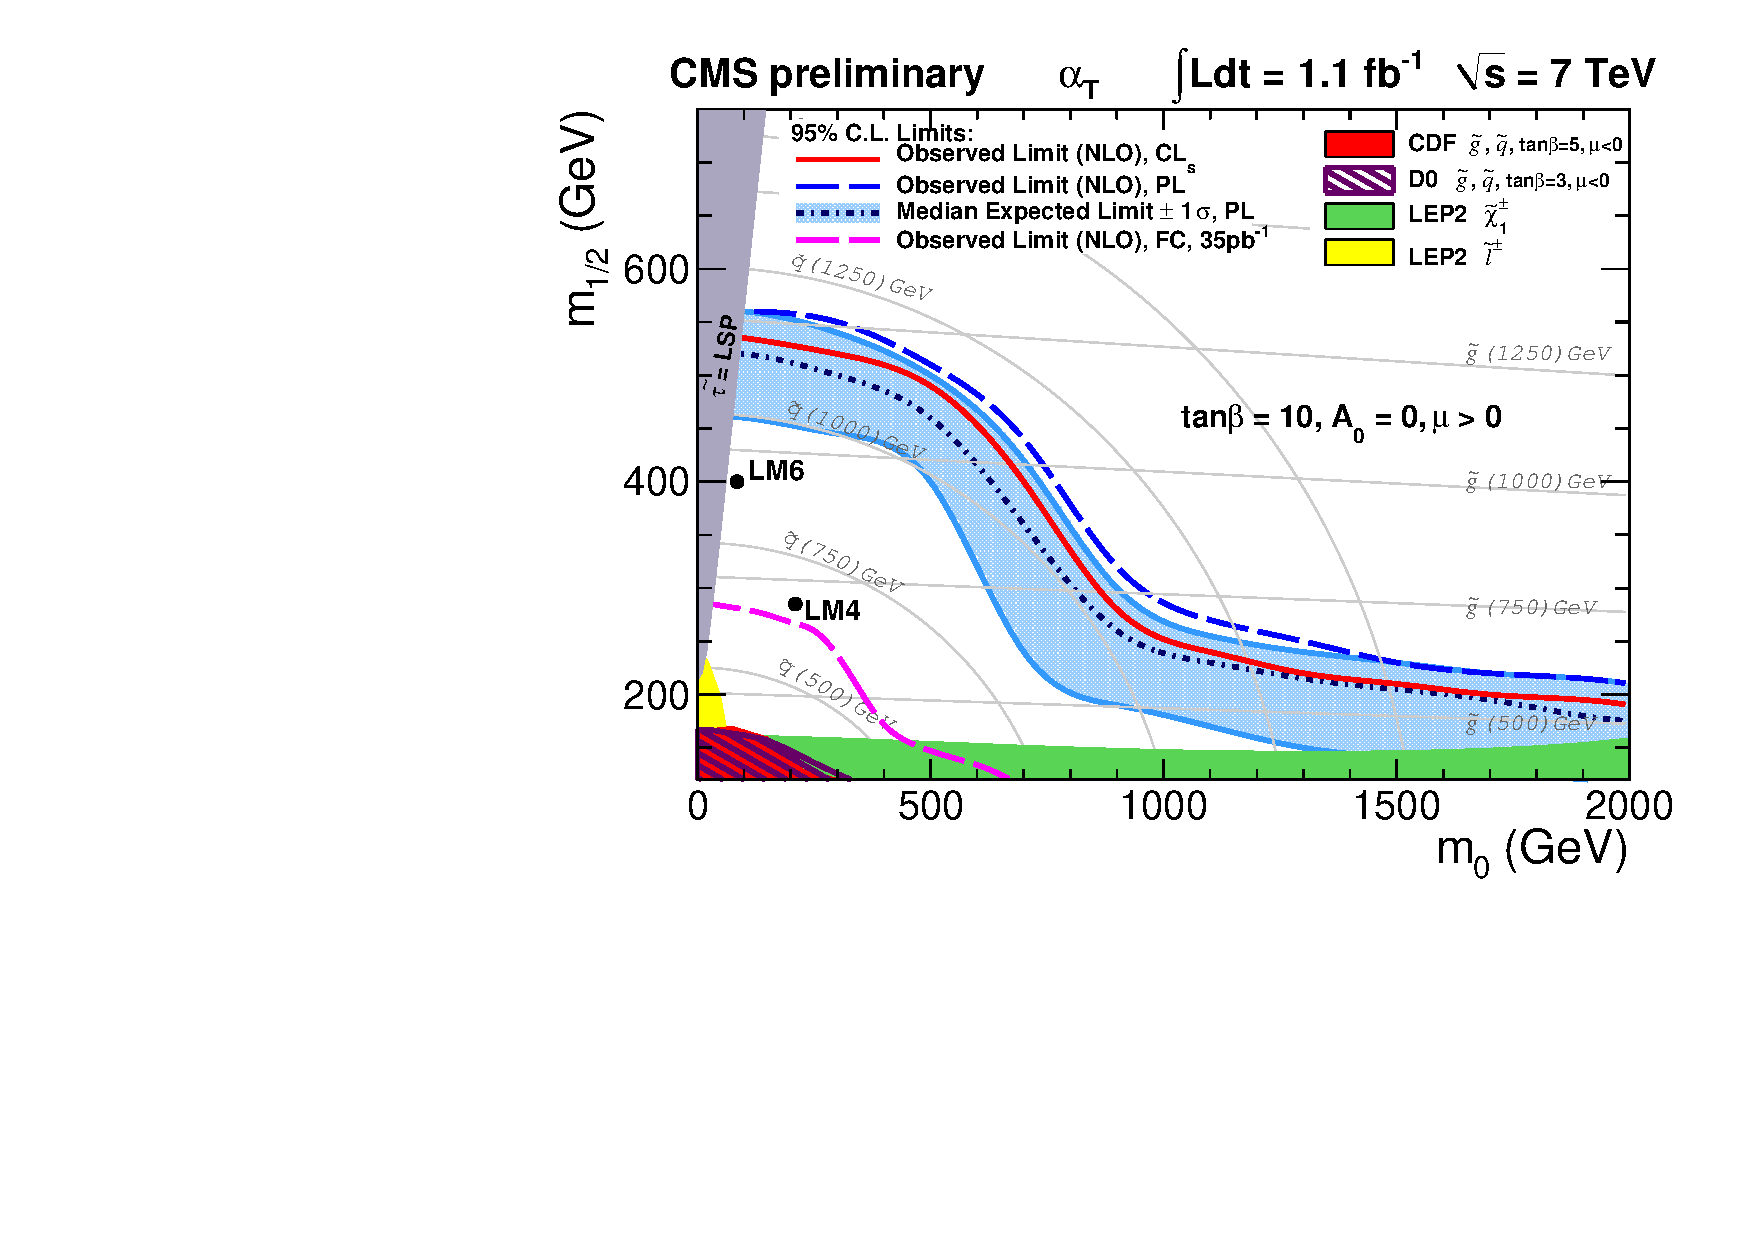
\includegraphics[width = 0.90\textwidth]{Figures/Analysis/PAS/RA1_ExclusionLimit_tanb10_def.pdf}
    \caption{\label{fig:cmssm} Observed and expected 95\% CL exclusion
      contours in the CMSSM ($m_0, m_{1/2}$) plane ($\tan \beta = 10,
      A_0 = 0, \mu > 0$) using NLO signal cross sections using the
      Profile Likelihood (PL) method. The expected limit is shown with
      its 68\% CL range.  The observed limit using the $\cls$ method is
      shown as well.  }
  \end{center}
\end{figure}


\section{Conclusion}

